\chapter{Game Theory of Adversarial Examples}
\label{chap:game}
\minitoc

In this chapter, we answer \textbf{Question 1: ``xxx''} by proving the existence of Mixed Nash equilibria in the adversarial example game when both the adversary and the classifier can use randomized strategies. First, we motivate in Section~\ref{sec:adv-problem} the necessity for using randomized strategies both with the attacker and the classifier. Then, we extend the work of~\cite{pydi2019adversarial}, by rigorously reformulating the adversarial risk as a linear optimization problem over distributions. In fact, we cast the adversarial risk minimization problem as a Distributionally Robust Optimization (DRO)~\citep{blanchet2019quantifying} problem for a well suited cost function. This formulation naturally leads us, in Section~\ref{sec:nash-eq}, to analyze adversarial risk minimization as a zero-sum game. We demonstrate that, in this game, the duality gap always equals $0$, meaning that it always admits approximate mixed Nash equilibria.  

Afterwards, we aim at designing an efficient algorithm to learn an optimally robust randomized classifier.
We focus on learning a finite mixture of classifiers. Drawing inspiration from robust optimization~\cite{sinha2017certifying} and subgradient methods~\cite{boyd2003subgradient}, we derive in Section~\ref{sec:algo} a first oracle algorithm to optimize a finite mixture. Then, following the line of work of~\citep{cuturi2013sinkhorn}, we introduce an entropic regularization to effectively compute an approximation of the optimal mixture. We validate our findings with experiments on simulated and real  datasets, namely CIFAR-10 an CIFAR-100~\cite{krizhevsky2009learning}.






\section{The Adversarial Attack Problem}
\label{sec:adv-problem}
\subsection{A Motivating Example}
\label{sec:motiv-ex}

\begin{figure*}[!ht]
    \centering
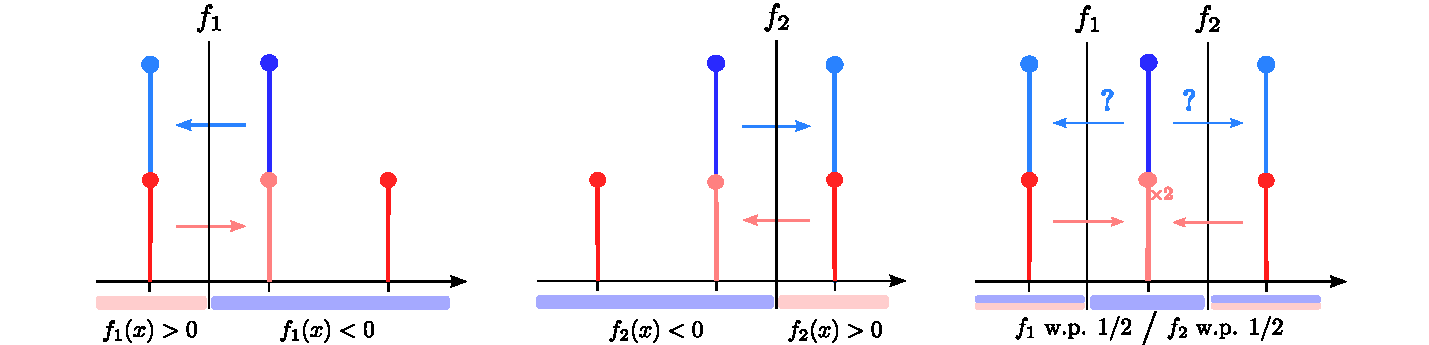
\includegraphics[width=\textwidth]{Images/Drawing-Intro-Mixte-Nash-on-a-line.pdf}   \caption{Motivating example: blue distribution represents label $-1$ and the red one, label $+1$.  The height of columns represents their mass. The red and blue arrows represent the attack on the given classifier. On left: deterministic classifiers ($f_1$ on the left, $f_2$ in the middle) for whose, the blue point can always be attacked. On right: a randomized classifier, where the attacker has a probability $1/2$ of failing, regardless of the attack it selects. }
    \label{fig:motivating_ex}
\end{figure*}
Consider the binary classification task illustrated in Figure~\ref{fig:motivating_ex}. We assume that all input-output pairs $(X,Y)$ are sampled from a distribution $\PP$ defined as follows
$$ 
\PP\left(Y =\pm 1\right)=1/2 \ \mbox{ and }\left\{
    \begin{array}{ll}
        \PP\left(X=0 \mid Y=-1\right) = 1 \\
        \PP\left(X= \pm 1 \mid Y=1\right) = 1/2 
    \end{array}
\right.
$$ 
Given access to $\PP$, the adversary aims to maximize the expected risk, but can only move each point by at most $1$ on the real line. In this context, we study two classifiers: $f_1(x) = -x -1/2$ and $f_2(x)=x-1/2$\footnote{$(X,Y) \sim \PP$ is misclassified by $f_i$ if and only if $f_i(X)Y \leq 0$}. Both $f_1$ and $f_2$ have a standard risk of $1/4$. In the presence of an adversary, the risk (\emph{a.k.a.} the adversarial risk) increases to $1$. Here, using a randomized classifier can make the system more robust. Consider $f$ where $f=f_1$ w.p. $1/2$ and $f_2$ otherwise. The standard risk of $f$ remains $1/4$ but its adversarial risk is $3/4<1$. Indeed, when attacking $f$, any adversary will have to choose between moving points from $0$ to $1$ or to $-1$. Either ways, the attack only works half of the time; hence an overall adversarial risk of $3/4$. Furthermore, if $f$ knows the strategy the adversary uses, it can always update the probability it gives to $f_1$ and $f_2$ to get a better (possibly deterministic) defense. For example, if the adversary chooses to always move $0$ to $1$, the classifier can set $f=f_1$ w.p. $1$ to retrieve an adversarial risk of $1/2$ instead of $3/4$. %In other words, if the adversary can only use a deterministic attack, then there exists no equilibrium in the game.

Now, what happens if the adversary can use randomized strategies, meaning that for each point it can flip a coin before deciding where to move? In this case, the adversary could decide to move points from $0$ to $1$ w.p. $1/2$ and to $-1$ otherwise. This strategy is still optimal with an adversarial risk of $3/4$ but now the classifier cannot use its knowledge of the adversary's strategy to lower the risk. We are in a state where neither the adversary nor the classifier can benefit from unilaterally changing its strategy. In the game theory terminology, this state is called a Mixed Nash equilibrium. %Previous works studying adversarial examples from the scope of game theory investigated the existence of Mixed Nash equilibria in restricted settings where the adversary can by reduced to a set of parameters~\citep{7533509,DBLP:journals/corr/abs-1906-02816,bose2021adversarial}. But, as pointed out in \citep{pinot2020randomization} and \citep{pydi2019adversarial}, studying the existence of a Mixed Nash equilibrium in a more general framework is a challenging open problem. In the present paper we tackle the following question.

\subsection{General setting}
Let us consider a loss function: $\loss:\Theta\times (\XX\times\YY)\to [0,\infty)$ satisfying the following set of assumptions.
\begin{assump}[Loss function]
\label{ass:loss}
1) The loss function $\loss$ is a non negative Borel measurable function. 2) For all $\theta\in\Theta$, $\loss(\theta,\cdot)$ is upper-semi continuous. 3) There exists $M>0$ such that for all $\theta\in\Theta$, $(x,y)\in\XX\times\YY$, $0\leq \loss(\theta,(x,y))\leq M$.
\end{assump}
It is usual to assume upper-semi continuity when studying optimization over distributions~\citep{villani2003topics,blanchet2019quantifying}. Furthermore, considering bounded (and positive) loss functions is also very common in learning theory~\citep{bartlett2002rademacher} and is not restrictive. 

In the adversarial examples framework, the loss of interest is the $0/1$ loss, for whose surrogates are misunderstood  and is the object of Chapter~\ref{chap:calibration}; hence it is essential that a $0/1$ loss satisfies Assumption~\ref{ass:loss}. In the binary classification setting (\emph{i.e.} $\YY=\{-1,+1\}$) a possible $0/1$ loss writes $\loss_{0/1}(\theta,(x,y)) = \mathbf{1}_{yf_\theta(x)\leq 0}$. Then, assuming that for all $\theta$, $f_\theta(\cdot)$ is continuous and for all $x$, $f_\cdot(x)$ is continuous, the $0/1$ loss satisfies Assumption~\ref{ass:loss}. In particular, it is the case for neural networks with continuous activation functions.


\subsection{Measure Theoretic Lemmas}

We first recall and prove some important lemmas about measure theory.
\begin{lemma}[Fubini's theorem]
\label{lem:fubini}
Let $\loss:\Theta\times(\XX\times\YY)\rightarrow [0,\infty)$ satisfying Assumption~\ref{ass:loss}. Then for all $\mu\in\mathcal{M}^1_+(\Theta)$, $\int \loss(\theta,\cdot)d\mu(\theta)$ is Borel measurable; for  $\QQ\in\mathcal{M}^1_+(\XX\times\YY)$, $\int \loss(\cdot,(x,y))d\QQ(x,y)$ is Borel measurable. Moreover: $\int \loss(\theta,(x,y))d\mu(\theta)d\QQ(x,y)=\int \loss(\theta,(x,y))d\QQ(x,y)d\mu(\theta)$
\end{lemma}

\begin{lemma}
\label{lem:usc1}
Let $\loss:\Theta\times(\XX\times\YY)\rightarrow [0,\infty)$ satisfying Assumption~\ref{ass:loss}.
Then for all $\mu\in\mathcal{M}^1_+(\Theta)$, $(x,y)\mapsto\int \loss(\theta,(x,y))d\mu(\theta)$ is upper semi-continuous and hence Borel measurable.  
\end{lemma}
\begin{proof}
Let $(x_n,y_n)_n$ be a sequence of $\XX\times\YY$ converging to $(x,y)\in\XX\times\YY$.  Let $M$ be an upper bound on the loss $\loss$. For all $\theta\in\Theta$, $M-\loss(\theta,\cdot)$ is non negative and lower semi-continuous. Then by Fatou's Lemma :
\begin{align*}
   \int M-\loss(\theta,(x,y))d\mu(\theta)&\leq\int \liminf_{n\to\infty}  M-\loss(\theta,(x_n,y_n))d\mu(\theta)\\
   &\leq  \liminf_{n\to\infty}  \int M-\loss(\theta,(x_n,y_n))d\mu(\theta) 
\end{align*}

We then have: $\int M- \loss(\theta,\cdot)d\mu(\theta)$ is lower semi-continuous and then $\int \loss(\theta,\cdot)d\mu(\theta)$ is upper-semi continuous.
\end{proof}


\begin{lemma}
\label{lem:usc2}

Let $\loss:\Theta\times(\XX\times\YY)\rightarrow [0,\infty)$ satisfying Assumption~\ref{ass:loss}.
Then for all $\mu\in\mathcal{M}^1_+(\Theta)$, $\QQ\mapsto\int \loss(\theta,(x,y))d\mu(\theta)d\QQ(x,y)$ is upper semi-continuous for the weak topology of measures. 
\end{lemma}
\begin{proof}
 $-\int \loss(\theta,\cdot)d\mu(\theta) $ is lower semi-continuous from Lemma~\ref{lem:usc1}. Then $M-\int \loss(\theta,\cdot)d\mu(\theta) $ is lower semi-continuous and non negative. Letus  denote $v$ this function. Let $(v_n)_n$ be a non-decreasing sequence of continuous bounded functions such that $v_n\to v$. Let $(\QQ_k)_k$ converge weakly towards $\QQ$. Then by monotone convergence theorem:
 
 \begin{align*}
     \int vd\QQ = \lim_n \int v_nd\QQ =\lim_n \lim_k\int v_nd\QQ_k\leq \liminf_k \int vd\QQ_k
 \end{align*}
 Then $\QQ\mapsto\int vd\QQ$ is lower semi-continuous and then 
 \begin{align*}
    \QQ\mapsto\int \loss(\theta,(x,y))d\mu(\theta)d\QQ(x,y)
 \end{align*}
  is upper semi-continuous for weak topology of measures. 
 \end{proof}



% \begin{lemma}
% \label{lem:measure-sup}
% Let $\loss:\Theta\times(\XX\times\YY)\rightarrow [0,\infty)$ satisfying Assumption~\ref{ass:loss}.
% Then for all $\mu\in\mathcal{M}^1_+(\Theta)$, $(x,y)\mapsto \sup_{(x',y'),d(x,x')\leq\varepsilon,y=y'} \int \loss(\theta,(x',y'))d\mu(\theta)$ is universally measurable (i.e. measurable for all Borel probability measures). And hence the adversarial risk is well defined. 
% \end{lemma}
% \begin{proof}
% Let $\phi :(x,y)\mapsto \sup_{(x',y'),d(x,x')\leq\varepsilon,y=y'} \int \loss(\theta,(x',y'))d\mu(\theta)$. Then for $u\in\bar{\mathbb{R}}$:
% \begin{align*}
% &\left\{\phi(x,y)>u\right\}\\
% &=\text{Proj}_1\left\{((x,y),(x',y'))\mid\int \loss(\theta,(x',y'))d\mu(\theta)-c_\varepsilon((x,y),(x',y'))>u\right\}
% \end{align*}
% By Lemma~\ref{lem:usc2}: $((x,y),(x',y'))\mapsto \int \loss(\theta,(x',y'))d\mu(\theta)-c_\varepsilon((x,y),(x',y'))$ is upper-semicontinuous hence Borel measurable. So its level sets are Borel sets, and by~\citet[Proposition 7.39]{bertsekas2004stochastic}, the projection of a Borel set is analytic. And then $\left\{\phi(x,y)>u\right\}$ universally measurable thanks to~\citet[Corollary 7.42.1]{bertsekas2004stochastic}. We deduce that $\phi$ is universally measurable.
% \end{proof}



\subsection{Adversarial Risk Minimization}
The standard risk for a single classifier $\theta$ associated with the loss $\loss$ satisfying Assumption~\ref{ass:loss} writes: $\risk(\theta):=\mathbb{E}_{(x,y)\sim \PP}\left[\loss(\theta,(x,y))\right]$. Similarly, the adversarial risk of $\theta$ at level $\varepsilon$ associated with the loss $\loss$ is defined as\footnote{For the well-posedness, see Lemma~\ref{lem:measure-sup}.}
\begin{align*}
    \risk_\varepsilon(\theta):=\mathbb{E}_{(x,y)\sim \PP}\left[\sup_{x'\in\XX,~d(x,x')\leq\varepsilon}\loss(\theta,(x',y))\right].
\end{align*}
 It is clear that $\risk_0(\theta) =\risk(\theta)$ for all $\theta$. We can generalize these notions with distributions of classifiers. In other terms the classifier is then randomized according to some distribution $\mu\in\mathcal{M}^1_+(\Theta)$. A classifier is randomized if for a given input, the output of the classifier is a probability distribution.
 The standard risk of a randomized classifier $\mu$ writes $\risk(\mu) = \mathbb{E}_{\theta\sim\mu}\left[\risk (\theta)\right]$. Similarly, the adversarial risk of the randomized classifier $\mu$ at level $\varepsilon$ is\footnote{This risk is also well posed (see Lemma~\ref{lem:measure-sup}).}
\begin{align*}
    \risk_\varepsilon(\mu):=\mathbb{E}_{(x,y)\sim \PP}\left[\sup_{x'\in\XX,~d(x,x')\leq\varepsilon}\mathbb{E}_{\theta\sim\mu}\left[\loss(\theta,(x',y))\right]\right].
\end{align*}
For instance, for the $0/1$ loss, the inner maximization problem, consists in maximizing the probability of misclassification for a given pair $(x,y)$. Note that $\risk(\delta_\theta)=\risk(\theta)$ and $\risk_\varepsilon(\delta_\theta)=\risk_\varepsilon(\theta)$. In the remainder of this section, we study the adversarial risk minimization problems with randomized and deterministic classifiers and denote
\begin{align}
\label{eq:advriskmin}
    \valuerand_\varepsilon:=\inf_{\mu\in\mathcal{M}^1_+(\Theta)} \risk_\varepsilon(\mu),~\valuedet_\varepsilon:=\inf_{\theta\in\Theta} \risk_\varepsilon(\theta)
\end{align}
Note that we can show that the standard risk infima are equal :  $\valuerand_0=\valuedet_0$. 
\begin{prop}
\label{prop:eqstandardrisk}
Let $\PP$ be a Borel probability distribution on $\XX\times\YY$, and $\loss$ a loss satisfying Assumption~\ref{ass:loss}, then:
\begin{align*}
        \inf_{\mu\in\mathcal{M}^1_+(\Theta)} \risk(\mu) =\inf_{\theta\in\Theta} \risk(\theta)
\end{align*}
\end{prop}
\begin{proof}
We have $\inf_{\mu\in\mathcal{M}^1_+(\Theta)} \risk(\mu) \leq \inf_{\theta\in\Theta} \risk(\theta)$. Now, let $\mu\in\mathcal{M}^1_+(\Theta)$, then:
\begin{align*}
    \risk(\mu)= \mathbb{E}_{\theta\sim\mu}(\risk(\theta))&\geq \essinf_\mu \mathbb{E}_{\theta\sim\mu} \left(\risk(\theta)\right)\\
    &\geq\inf_{\theta\in\Theta} \risk(\theta).
\end{align*}
where $\essinf$ denotes the essential infimum.
\end{proof}
\begin{rmq}
No randomization is needed for minimizing the standard risk. Denoting $\mathcal{V}$ this common value, we also have the following inequalities for any $\varepsilon>0$, $\mathcal{V}\leq \valuerand_\varepsilon\leq \valuedet_\varepsilon$.
\end{rmq}



\subsection{Distributional Formulation of the Adversarial Risk} 

To account for the possible randomness of the adversary, we rewrite the adversarial attack problem as a convex optimization problem over distributions. Let us first introduce the set of adversarial distributions.
\begin{definition}[Set of adversarial distributions]
Let $\PP$ be a Borel probability distribution on $\XX\times\YY$ and $\varepsilon>0$. We define the set of adversarial distributions as
\begin{align*}
\mathcal{A}_{\varepsilon}&(\PP) := \left\{\QQ\in\mathcal{M}^+_1(\XX\times\YY)\mid\exists \gamma\in\mathcal{M}^+_1\left((\XX\times\YY)^2\right),\right.\\
&\left.d(x,x')\leq\varepsilon,~y=y'~~ \gamma\text{-a.s.},~\Pi_{1\sharp}\gamma=\PP,~\Pi_{2\sharp}\gamma=\QQ\right\} 
\end{align*}
where $\Pi_i$ denotes the projection on the $i$-th component, and $g_\sharp$ the push-forward measure by a measurable function $g$.
\end{definition}
An attacker that can move the initial distribution $\PP$ anywhere in $\mathcal{A}_\varepsilon(\PP)$ is not applying a point-wise deterministic perturbation as considered in the standard adversarial risk. %For every point $(x,y)$ in the support of $\PP$, the attacker is allowed to move $(x,y)$ according to a ``random mapping'' in the ball of radius $\varepsilon$, and not to a single other point $(x',y)$ like the usual attacker in adversarial attacks. 
In other words, for a point $(x,y)\sim\PP$, the attacker could choose a distribution $q(\cdot\mid(x,y))$ whose support is included in $\{(x',y')\mid d(x,x')\leq \epsilon,~y=y'\}$ from which he will sample the adversarial attack. In this sense, we say the attacker is allowed to be randomized.
% This set allows to move every single point in the support of $\PP$ and moving its mass everywhere as far as the perturbation is smaller than $\varepsilon$ and does not change the `true' label. In this problem, the attacker can then play randomized strategies to move the samples inside the balls of radius $\varepsilon$. \textcolor{red}{Pas hyper limpide je trouve}

\textbf{Link with DRO.} We immediately remark that $\mathcal{A}_\varepsilon(\PP)$ corresponds to the Wasserstein-$\infty$ set associated with
the cost
\begin{align*}
    d'((x,y),(x',y'))\mapsto \left\{
        \begin{array}{ll}
            d(x,x') & \mbox{if } y = y'\\
            +\infty & \mbox{otherwise.}
        \end{array}
    \right.
\end{align*}
Such a set can be defined from usual (not $\infty$) Wasserstein uncertainty sets:  for an arbitrary $\varepsilon>0$, we define the cost $c_\varepsilon$ as follows
\begin{align*}
c_\varepsilon((x,y),(x',y')) := \left\{
    \begin{array}{ll}
        0 & \mbox{if } d(x,x')\leq\varepsilon\mbox{ and }y = y'\\
        +\infty & \mbox{otherwise.}
    \end{array}
\right.
\end{align*}
This cost is lower semi-continuous and penalizes to infinity perturbations that change the label or move the input by a distance greater than $\varepsilon$. As Proposition~\ref{prop:wass_ball} shows, the Wasserstein ball associated with $c_\varepsilon$ is equal to $\mathcal{A}_{\varepsilon}(\PP)$.
\begin{prop}
\label{prop:wass_ball}
Let $\PP$ be a Borel probability distribution on $\XX\times\YY$ and $\varepsilon>0$ and $\eta\geq 0$, then
    $\mathcal{B}_{c_\varepsilon}(\PP,\eta) =\mathcal{A}_{\varepsilon}(\PP)$.
Moreover, $\mathcal{A}_{\varepsilon}(\PP)$ is convex and compact for the weak topology of $\mathcal{M}^+_1(\XX\times\YY)$.
\end{prop}
\begin{proof}
Let $\eta>0$. Let $\QQ\in\mathcal{A}_\varepsilon(\PP)$. There exists $\gamma\in
\mathcal{M}^+_1\left((\XX\times\YY)^2\right)$ such that, $d(x,x')\leq\varepsilon$, $y=y'$ $\gamma$-almost surely, and $\Pi_{1\sharp}\gamma=\PP$, and $\Pi_{2\sharp}\gamma=\QQ$. Then $\int c_\varepsilon d \gamma = 0\leq \eta$. Then, $W_{c_\varepsilon}(\PP,\QQ)\leq \eta$, and $\QQ\in\mathcal{B}_{c_\varepsilon}(\PP,\eta)$. Reciprocally, let $\QQ\in\mathcal{B}_{c_\varepsilon}(\PP,\eta)$. Then, since the infimum is attained in the Wasserstein definition, there exists $\gamma\in
\mathcal{M}^+_1\left((\XX\times\YY)^2\right)$ such that $\int c_\varepsilon d \gamma \leq \eta$. Since $c_\varepsilon((x,x'),(y,y'))=+\infty$ when $d(x,x')>\varepsilon$ and $y\neq y'$, we deduce that, $d(x,x')\leq\varepsilon$ and $y=y'$, $\gamma$-almost surely. Then $\QQ\in\mathcal{A}_\varepsilon(\PP)$. We have then shown that: $\mathcal{A}_\varepsilon(\PP)=\mathcal{B}_{c_\varepsilon}(\PP,\eta)$.

The convexity of $\mathcal{A}_\varepsilon(\PP)$ is  immediate from the relation with the Wasserstein uncertainty set.

Let us show first that $\mathcal{A}_\varepsilon(\PP)$ is relatively compact for the weak topology. To do so we will show that $\mathcal{A}_\varepsilon(\PP)$ is tight and apply Prokhorov theorem. Let $\delta>0$, $(\XX\times \YY,d\oplus d')$ being a Polish space, $\{\PP\}$ is tight then there exists $K_\delta$ compact such that $\PP(K_\delta)\geq1-\delta$.
Let $\Tilde{K}_\delta:=\left\{(x',y')\mid \exists (x,y)\in K_\delta,~ d(x',x)\leq\varepsilon,~y=y'\right\}$.  Recalling that $(\XX,d)$ is proper (i.e. the closed balls are compact), so $\Tilde{K}_\delta$ is compact. Moreover for $\QQ\in\mathcal{A}_\varepsilon(\PP)$, $\QQ(\Tilde{K}_\delta)\geq \PP(K_\delta)\geq 1-\delta$. And then, Prokhorov's theorem holds, and $\mathcal{A}_\varepsilon(\PP)$ is relatively compact for the weak topology.

Let us now prove that $\mathcal{A}_\varepsilon(\PP)$ is closed to conclude.  Let $(\QQ_n)_n$ be a sequence of $\mathcal{A}_\varepsilon(\PP)$ converging towards some $\QQ$ for weak topology. For each $n$, there exists $\gamma_n\in \mathcal{M}^1_+(\XX\times\YY)$ such that $d(x,x')\leq\varepsilon$ and $y=y'$ $\gamma_n$-almost surely and $\Pi_{1\sharp}\gamma_n=\PP$, $\Pi_{2\sharp}\gamma_n=\QQ_n$. $\{\QQ_n,n\geq0\}$ is relatively compact, then tight, then $\bigcup_n \Gamma_{\PP,\QQ_n}$ is tight, then relatively compact by Prokhorov's theorem. $(\gamma_n)_n\in\bigcup_n \Gamma_{\PP,\QQ_n}$, then up to an extraction,  $\gamma_n\to\gamma$. Then $d(x,x')\leq\varepsilon$ and $y=y'$ $\gamma$-almost surely, and by continuity, $\Pi_{1\sharp}\gamma=\PP$ and by continuity, $\Pi_{2\sharp}\gamma=\QQ$. And hence $\mathcal{A}_\varepsilon(\PP)$ is closed.

Finally $\mathcal{A}_\varepsilon(\PP)$ is a convex compact set for the weak topology. 
\end{proof}




% Next proposition shows that the set $\mathcal{A}_{\varepsilon}(\PP)$ satisfies interesting topological properties. See proof in Appendix~\ref{prv:a_eps}.
% \begin{prop}
% \label{prop:a_eps}
% Let $\PP$ be a Borel probability distribution on $\XX\times\YY$ and $\varepsilon>0$. $\mathcal{A}_{\varepsilon}(\PP)$ is convex and compact for the weak topology of $\mathcal{M}^+_1(\XX\times\YY)$.
% \end{prop}
Thanks to this result, we can reformulate the adversarial risk as the value of a convex problem over $\mathcal{A}_\varepsilon(\PP)$. %See proof in Appendix~\ref{prv:duality-rand}.
\begin{prop} 
\label{prop:dro_adv}
Let $\PP$ be a Borel probability distribution on $\XX\times\YY$ and $\mu$ a Borel probability distribution on $\Theta$. Let $\loss:\Theta\times(\XX\times\YY)\to [0,\infty)$ satisfying Assumption~\ref{ass:loss}. Let $\varepsilon>0$. Then:
\begin{align}
\label{eq:dro-adv}
\risk_\varepsilon(\mu)= \sup_{\QQ\in \mathcal{A}_{\varepsilon}(\PP)}\mathbb{E}_{(x',y')\sim\QQ,\theta\sim\mu}\left[\loss(\theta,(x',y'))\right].
\end{align}
The supremum is attained. Moreover $\QQ^*\in \mathcal{A}_{\varepsilon}(\PP)$ is an optimum of Problem~\eqref{eq:dro-adv} if and only if there exists $\gamma^*\in\mathcal{M}^+_1\left((\XX\times\YY)^2\right)$ such that: $\Pi_{1\sharp}\gamma^*=\PP$, $\Pi_{2\sharp}\gamma^*=\QQ^*$, $d(x,x')\leq\varepsilon$, $y=y'$ and  $\loss(x',y')=\sup_{\substack{u\in\XX,d(x,u)\leq\varepsilon}}\loss(u,y)$ $\gamma^*$-almost surely.
\end{prop}

\begin{proof}
Let $\mu\in\mathcal{M}^1_+(\Theta)$. Let us define $\Tilde{f}$ as
\begin{align*}
    \Tilde{f}:((x,y),(x',y'))\mapsto \mathbb{E}_{\theta\sim\mu}\left[\loss(\theta,(x,y))\right]-c_\varepsilon((x,y),(x',y'))\quad. 
\end{align*}
 $\Tilde{f}$ is upper-semi continuous, hence upper semi-analytic. Then, by upper semi continuity of $\mathbb{E}_{\theta\sim\mu}\left[\loss(\theta,\cdot)\right]$ on the compact $\{(x',y')\mid~d(x,x')\leq\varepsilon,y=y'\}$ and~\citep[Proposition 7.50]{bertsekas2004stochastic}, there exists a universally measurable mapping $T$ such that $\mathbb{E}_{\theta\sim\mu}\left[\loss(\theta,T(x,y))\right]=\sup_{(x',y'),~d(x,x')\leq\varepsilon,y=y'}\mathbb{E}_{\theta\sim\mu}\left[\loss(\theta,(x,y))\right]$.  Let $\QQ = T_{\sharp}\PP$, then $\QQ\in\mathcal{A}_\varepsilon(\PP)$. And then 
 \begin{align*}
      \mathbb{E}_{(x,y)\sim\PP}&\left[\sup_{(x',y'),~d(x,x')\leq\varepsilon,y=y'}\mathbb{E}_{\theta\sim\mu}\left[\loss(\theta,(x',y'))\right]\right]\\
      &\leq \sup_{\QQ\in\mathcal{A}_\varepsilon(\PP)}\mathbb{E}_{(x,y)\sim\QQ}\left[\mathbb{E}_{\theta\sim\mu}\left[\loss(\theta,(x,y))\right]\right]\quad.
\end{align*}


Reciprocally, let $\QQ\in\mathcal{A}_\varepsilon(\PP)$. There exists $\gamma\in\mathcal{M}^1_+((\XX\times\YY)^2)$, such that $d(x,x')\leq\varepsilon$ and $y=y'$ $\gamma$-almost surely, and, $\Pi_{1\sharp}\gamma=\PP$ and  $\Pi_{2\sharp}\gamma=\QQ$. Then:
$\mathbb{E}_{\theta\sim\mu}\left[\loss(\theta,(x',y'))\right]\leq\sup_{(u,v),~d(x,u)\leq\varepsilon,y=v}\mathbb{E}_{\theta\sim\mu}\left[\loss(\theta,(u,v))\right]$ $\gamma$-almost surely. Then, we deduce that:
\begin{align*}
    \mathbb{E}_{(x',y')\sim\QQ}&\left[\mathbb{E}_{\theta\sim\mu}\left[\loss(\theta,(x',y'))\right]\right]\\
    & =     \mathbb{E}_{(x,y,x',y')\sim\gamma}\left[\mathbb{E}_{\theta\sim\mu}\left[\loss(\theta,(x',y'))\right]\right] \\
    &\leq\mathbb{E}_{(x,y,x',y')\sim\gamma}\left[\sup_{(u,v),~d(x,u)\leq\varepsilon,y=v}\mathbb{E}_{\theta\sim\mu}\left[\loss(\theta,(u,v))\right]\right]\\
    &\leq\mathbb{E}_{(x,y)\sim\PP}\left[\sup_{(u,v),~d(x,u)\leq\varepsilon,y=v}\mathbb{E}_{\theta\sim\mu}\left[\loss(\theta,(u,v))\right]\right]
\end{align*}

Then we deduce the expected result:
\begin{align*}
\risk_\varepsilon(\mu)= \sup_{\QQ\in\mathcal{A}_\varepsilon(\PP)}\mathbb{E}_{(x,y)\sim\QQ}\left[\mathbb{E}_{\theta\sim\mu}\left[\loss(\theta,(x,y))\right]\right]
\end{align*}
Let us show that the optimum is attained. $\QQ\mapsto\mathbb{E}_{(x,y)\sim\QQ}\left[\mathbb{E}_{\theta\sim\mu}\left[\loss(\theta,(x,y))\right]\right]$ is upper semi continuous by Lemma~\ref{lem:usc2} for the weak topology of measures, and $\mathcal{A}_\varepsilon(\PP)$ is compact by Proposition~\ref{prop:wass_ball}, then by Prop. 7.32 from ~\citep{bertsekas2004stochastic}, the supremum is attained for a certain $\QQ^*\in\mathcal{A}_\varepsilon(\PP)$. 

\end{proof}

The adversarial attack problem is a DRO problem for the cost $c_\varepsilon$.
Proposition~\ref{prop:dro_adv} means that, against a fixed classifier $\mu$, the randomized attacker that can move the distribution in $\mathcal{A}_\varepsilon(\PP)$ has exactly the same power as an attacker that moves every single point $x$ in the ball of radius $\varepsilon$.  By Proposition~\ref{prop:dro_adv}, we also  deduce that the adversarial risk can be casted as a linear optimization problem over distributions.

\begin{rmq}
  In a recent work,~\citep{pydi2019adversarial} proposed a similar adversary using Markov kernels but left as an open question the link with the classical adversarial risk, due to measurability issues. Proposition~\ref{prop:dro_adv} solves these issues. The result is similar to~\citep{blanchet2019quantifying}. Although we believe its proof might be extended for infinite valued costs,~\citep{blanchet2019quantifying} did not treat that case. We provide an alternative proof in this special case. 
\end{rmq}


 %In the next section we show how Proposition~\ref{prop:dro_adv} helps casting the adversarial risk minimization problem as a game between the classifier and the attacker for which we study the Nash equilibria.

% \paragraph{Link with distributionally robust optimization (DRO). } The optimization problem over $\mathcal{A}_\varepsilon(\PP)$ is very close to a DRO problem ~\citep{blanchet2019quantifying}. 
% When $(\mathcal{Z},d)$ a Polish space and $c:\mathcal{Z}^2\rightarrow\mathbb{R}^+\cup\{+\infty\}$ be a lower semi-continuous function, for $\PP,\QQ\in\mathcal{M}^+_1(\mathcal{Z})$ , the primal Optimal Transport problem is defined as:
% \begin{align*}
%   W_c(\PP,\QQ):=\inf_{\gamma\in\Gamma_{\PP,\QQ}}  \int_{\mathcal{Z}^2} c(z,z')d\gamma(z,z')
% \end{align*}
% with $\Gamma_{\PP,\QQ}:=\left\{\gamma\in\mathcal{M}^+_1(\mathcal{Z}^2)\mid~\Pi_{1\sharp}\gamma = \PP,~\Pi_{2\sharp}\gamma = \QQ \right\}$. When $\delta>0$ and for $\PP\in\mathcal{M}^+_1(\mathcal{Z})$, the associated Wasserstein uncertainty set is defined as: 
% \begin{align*}
%     \mathcal{B}_{c}(\PP,\delta) := \left\{\QQ\in \mathcal{M}^+_1(\mathcal{Z})\mid W_c(\PP,\QQ)\leq \delta\right\}
% \end{align*}
% A DRO problem is a linear optimization problem over Wasserstein uncertainty sets. We can show that $\mathcal{A}_{\varepsilon}(\PP)$ is actually a Wasserstein uncertainty set for a well-suited cost on $(\XX\times\YY)^2$. For $\varepsilon$, we define $c_\varepsilon$ the cost defined as $c_\varepsilon((x,y),(x',y')) = d(x,x')$ if $d(x,x')\leq\varepsilon$ and $y = y'$, and $+\infty$ otherwise. The cost for perturbations that changing the label and the input by a distance greater than $\varepsilon$ would be infinite. Next proposition link the Wasserstein ball associated with $c_\varepsilon$ and $\mathcal{A}_{\varepsilon}(\PP)$.
% \begin{prop}
% Let $\PP$ be a Borel probability distribution on $\XX\times\YY$ and $\varepsilon>0$ and $\delta>\varepsilon$, then:
% \begin{align*}
%     \mathcal{B}_{c_\varepsilon}(\PP,\delta) =\mathcal{A}_{\varepsilon}(\PP)
% \end{align*}
% \end{prop}
% One may have thought to apply directy Theorem 1 from~\citep{blanchet2019quantifying} to prove Proposition~\ref{prop:dro_adv}; however, the result holds for real-valued costs (i.e. $<\infty$). We believe it can be extended to infinite valued costs, but it is out of the scope of this paper. 
% \begin{prop} 
% \label{prop:dro_adv}
% Let $\PP$ be a Borel probability distribution on $\XX\times\YY$ and $\mu$ a Borel probability distribution on $\Theta$. Let $l:\Theta\times(\XX\times\YY)\to [0,+\infty]$ satisfying Assumption~\ref{ass:loss}. Let $\varepsilon>0$. Then:
% \begin{align*}
% \risk^\epsilon(\mu)= \sup_{\QQ\in \mathcal{A}_{\varepsilon}(\PP)}\mathbb{E}_{(x',y')\sim\QQ,\theta\sim\mu}\left[\loss(\theta,(x',y'))\right]
% \end{align*}
% \begin{align*}
% \mathbb{E}_{(x,y)\sim \PP}\left[\sup_{\substack{u\in\XX,\\d(x,u)\leq\varepsilon}}l(u,y)\right] = \sup_{\QQ\in \mathcal{A}_{\varepsilon}(\PP)}\mathbb{E}_{(x',y')\sim\QQ}\left[\loss(x',y')\right]
% \end{align*}
% The supremum is attained. Moreover $\QQ^*\in \mathcal{A}_{\varepsilon}(\PP)$ is an optimum if and only if there exists $\gamma^*\in\mathcal{M}^+_1\left((\XX\times\YY)^2\right)$ such that: $\Pi_{1\sharp}\gamma^*=\PP$, $\Pi_{2\sharp}\gamma^*=\QQ^*$, $d(x,x')\leq\varepsilon$, $y=y'$ and  $l(x',y')=\sup_{\substack{u\in\XX,d(x,u)\leq\varepsilon}}l(u,y)$ $\gamma^*$-almost surely.
% \end{prop}


% say that the program is linear blabla + link with latest pydi
% One can also recast the adversarial problem as an infinite linear problem:
% \begin{align*}
%   \risk^\epsilon(\mu) = \sup_{\gamma\in \Tilde{\mathcal{A}}_{\varepsilon}(\PP)}\mathbb{E}_{(x,y,x',y')\sim\gamma}\left[\loss(x',y')\right]
% \end{align*}

% where 
% \begin{align*}
% \Tilde{\mathcal{A}}_{\varepsilon}&(\PP) := \left\{\gamma\in\mathcal{M}^+_1\left((\XX\times\YY)^2\right)\mid~\Pi_{1\sharp}\gamma=\PP\right.\\
% &\left.\int \delta\{d(x,x')\leq\varepsilon,~y=y'\}d\gamma(x,y,x'y')=0\right\}
% \end{align*}
% with $\delta$ is the indicator function. Remark that $\mathcal{A}_{\varepsilon}(\PP)=\Pi_{2\sharp}\Tilde{\mathcal{A}}_{\varepsilon}(\PP)$

% \paragraph{A primal-dual formulation of risk minimization.}Let $\mu\in\mathcal{M}^1_+(\Theta)$ a possibly randomized classifier. Thanks to Proposition~\ref{prop:dro_adv}, we have that for $\varepsilon>0$:
% \begin{align*}
%     \risk^\varepsilon(\mu)=\sup_{\QQ\in\mathcal{A}_{\varepsilon}(\PP)}\mathbb{E}_{(x,y)\sim\QQ,\theta\sim\mu}\left[\loss(\theta,(x,y))\right]
% \end{align*}
% Following the definition of the risk minimization objective,  one can define the dual of this problem for randomized classifiers:
% \begin{align}
%     \sup_{\QQ\in\mathcal{A}_{\varepsilon}(\PP)}\inf_{\mu\in\mathcal{M}^1_+(\Theta)}\mathbb{E}_{(x,y)\sim\QQ,\theta\sim\mu}\left[\loss(\theta,(x,y))\right]
% \label{eq:dual_pb}
% \end{align}
% and its analog for deterministic classifiers:
% \begin{align*}
%     \sup_{\QQ\in\mathcal{A}_{\varepsilon}(\PP)}\inf_{\theta\in\Theta}\mathbb{E}_{(x,y)\sim\QQ}\left[\loss(\theta,(x,y))\right]
% \end{align*}
% Then, one can notice that the dual problems for deterministic and randomized classifiers are equivalent\footnote{See Appendix XXX for more details}. We denote $\dualvalue^\varepsilon$ the value of the dual problem.
% Weak duality is always satisfied:
% \begin{align}
% \label{eq:weak_duality}
% \dualvalue^\varepsilon\leq \valuerand^\varepsilon\leq \valuedet^\varepsilon
% \end{align}
% We will show in the next section, that, under Assumption~\ref{ass:loss}, strong duality always holds for this min-max problem.


% \begin{definition}[Optimal transport problem] Let $(\mathcal{Z},d)$ be a Polish space. Let $c:\mathcal{Z}^2\rightarrow\mathbb{R}^+\cup\{+\infty\}$ be a lower semi-continuous function. For $\PP,\QQ\in\mathcal{M}^+_1(\mathcal{Z})$, the primal optimal transport problem is defined as:
% \begin{align*}
%   W_c(\PP,\QQ):=\inf_{\gamma\in\Gamma_{\PP,\QQ}}  \int_{\mathcal{Z}^2} c(z,z')d\gamma(z,z')
% \end{align*}
% with $\Gamma_{\PP,\QQ}:=\left\{\gamma\in\mathcal{M}^+_1(\mathcal{Z}^2)\mid~\Pi_{1\sharp}\gamma = \PP,~\Pi_{2\sharp}\gamma = \QQ \right\}$ 
% \end{definition}

% We now define the Wasserstein uncertainty set.
% \begin{definition}[Wasserstein uncertainty set]Let $(\mathcal{Z},d)$ be a Polish space. Let $c:\mathcal{Z}^2\rightarrow\mathbb{R}^+\cup\{+\infty\}$ be a lower semi-continuous function. For $\PP\in\mathcal{M}^+_1(\mathcal{Z})$ and $\delta>0$, we define the Wasserstein uncertainty set:
% \begin{align*}
%     \mathcal{B}_{c}(\PP,\delta) := \left\{\QQ\in \mathcal{M}^+_1(\mathcal{Z})\mid W_c(\PP,\QQ)\leq \delta\right\}
% \end{align*}

% \end{definition}
% We recall that since for all $\PP$, $\QQ\mapsto W_c(\PP,\QQ)$ is convex, the Wasserstein uncertainty sets are convex. Moreover, $\QQ\mapsto W_c(\PP,\QQ)$ is a lower semi-continuous function for the weak topology then $\mathcal{B}_{c}(\PP,\delta)$ is a closed set. Under some mild assumptions the Wasserstein uncertainty balls are compact for weak topology. See details in App. 

% We now connect this problem to that of designing adversarial attacks for a given classification task. Let $(\XX,d_{\XX})$ be a proper Polish metric space representing the input space. Let $\YY=\{1,\dots,K\}$ be the labels set, endowed with trivial metric  $d_{\YY}(y,y') = \mathrm{1}_{y\neq y'}$. Then the space  $(\XX\times\YY,d_\XX\oplus d_\YY)$ is a proper Polish space. We denote $c_\varepsilon$ the cost defined as $c_\varepsilon((x,y),(x',y')) = d(x,x')$ if $d(x,x')\leq\varepsilon$ and $y = y'$, and $+\infty$. The cost for perturbations that changing the label and the input by a distance greater than $\varepsilon$ would be infinite. For $\delta>\epsilon$, next proposition shows that $\mathcal{B}_{c_{\varepsilon}}(\PP,\delta)$ allows all perturbations smaller than $\epsilon$.

% \begin{prop}
% Let $\PP$ be a distribution on $\XX\times\YY$ and $\varepsilon>0$ and $\delta>\varepsilon$, then:
% \begin{align*}
% \mathcal{B}_{c_{\varepsilon}}&(\PP,\delta) = \left\{\QQ\in\mathcal{M}^+_1(\XX\times\YY)\mid\exists \gamma\in\mathcal{M}^+_1\left((\XX\times\YY)^2\right),\right.\\
% &\left.d(x,x')\leq\varepsilon,~y=y'~~ \gamma\text{-a.s.},~\Pi_{1\sharp}\gamma=\PP,~\Pi_{2\sharp}\gamma=\QQ\right\} 
% \end{align*}
% This set will be denoted $\mathcal{A}_\varepsilon(\PP)$ this set. The set $\mathcal{A}_\varepsilon(\PP)$ is a convex and compact for weak topology.
% \end{prop}
 
% \begin{prop} 
% \label{prop:dro_adv}
% Let $\PP$ be a distribution on $\XX\times\YY$. Let $l:\XX\times\YY\mapsto\mathbb{R}$ be an upper semi continuous measurable function. We suppose that $l\in L^1(\PP)$. Let $\varepsilon>0$. Then:
% \begin{align*}
% \mathbb{E}_{(x,y)\sim \PP}\left[\sup_{\substack{u\in\XX,\\d(x,u)\leq\varepsilon}}l(u,y)\right] = \sup_{\QQ\in \mathcal{A}_{\varepsilon}(\PP)}\mathbb{E}_{(x',y')\sim\QQ}\left[\loss(x',y')\right]
% \end{align*}
% The supremum is attained. Moreover $\QQ^*\in \mathcal{A}_{\varepsilon}(\PP)$ is an optimum if and only if there exists $\gamma^*\in\mathcal{M}^+_1\left((\XX\times\YY)^2\right)$ such that: $\Pi_{1\sharp}\gamma^*=\PP$, $\Pi_{2\sharp}\gamma^*=\QQ^*$, $d(x,x')\leq\varepsilon$, $y=y'$ and  $l(x',y')=\sup_{\substack{u\in\XX,d(x,u)\leq\varepsilon}}l(u,y)$ $\gamma^*$-almost surely.
% \end{prop}

% \laurent{can we prove this result without using blanchet, i think so no? It is the result of blanchet}

\section{Nash Equilibria in the Adversarial Game}
\label{sec:nash-eq}

\subsection{Adversarial Attacks as a Zero-Sum Game}

Thanks to Proposition~\ref{sec:adv-problem}, the adversarial risk minimization problem can  be seen as a two-player zero-sum game that writes as follows,
\begin{align}
    \inf_{\mu\in\mathcal{M}^1_+(\Theta)} \sup_{\QQ\in\mathcal{A}_{\varepsilon}(\PP)}\mathbb{E}_{(x,y)\sim\QQ,\theta\sim\mu}\left[\loss(\theta,(x,y))\right].
\label{eq:primal_pb}
\end{align}
In this game, the classifier's objective is to find the best distribution $\mu \in \mathcal{M}_1^+(\Theta)$ while the adversary is manipulating the data distribution. For the classifier, solving the infimum problem in Equation~\eqref{eq:primal_pb} simply amounts to solving the adversarial risk minimization problem -- Problem~\eqref{eq:advriskmin}, whether the classifier is randomized or not. Then, given a randomized classifier $\mu \in \mathcal{M}_1^+(\Theta)$, the goal of the attacker is to find a new data-set distribution $\mathbb{Q}$ in the set of adversarial distributions $\mathcal{A}_{\varepsilon}(\PP)$ that maximizes the risk of $\mu$. More formally, the adversary looks for $$\mathbb{Q} \in \argmaxB_{\QQ\in\mathcal{A}_{\varepsilon}(\PP)} \mathbb{E}_{(x,y)\sim\QQ,\theta\sim\mu}\left[\loss(\theta,(x,y))\right]. $$
In the game theoretic terminology, $\mathbb{Q}$ is also called the best response of the attacker to the classifier $\mu$.

\begin{rmq}
Note that for a given classifier $\mu$ there always exists a ``deterministic'' best response, i.e. every single point $(x,y)$ is mapped to another single point $T(x,y)$. Let $T:\XX\times\YY\to\XX\times\YY$ be defined such that for all $(x,y)\in\XX\times\YY$, $\EE_{\theta\sim\mu}\left[\loss(T(x,y))\right] = \sup_{x',~d(x,x')\leq\varepsilon}\EE_{\theta\sim\mu}\left[ L(x',y)\right]$. Thanks to Prop. 7.50 from ~\citep{bertsekas2004stochastic}, $T$ is $\PP$-measurable. Moreover, we get that $\QQ = (T,id)_\sharp \PP$ belongs to the best response to $\mu$. Therefore, $T$ is the optimal ``deterministic'' attack against the classifier $\mu$.
\end{rmq}


%The classifier cannot play a best response against the attacker since the attacker is usually unknown. Thanks to the inequality~\eqref{eq:weak_duality}, the lowest risk, the classifier can hope is $\mathcal{D}^\varepsilon$. But as seen in the motivating example, it might not been attained by a deterministic classifier. We show in this section, that randomized classifiers can approach $\mathcal{D}^\varepsilon$ arbitrary closely.

%\begin{itemize}
%    \item 3.1 0 sum game , mininmizer = jeu
%    \item in this game: classifier oblivious to the attacker -> standard setting, attacker is whitebox
%    \item 3.2 dual formulation: sup inf, attackant adaptif, and Black box attacks
%    \item 3.3 evaluating duality gap
%\end{itemize}

\subsection{Dual Formulation of the Game}

Every zero sum game has a dual formulation that allows a deeper understanding of the framework. Here, from Proposition~\ref{prop:dro_adv}, we can define the dual problem of adversarial risk minimization for randomized classifiers. This dual problem also characterizes a two-player zero-sum game that writes as follows,
\begin{align}
    \sup_{\QQ\in\mathcal{A}_{\varepsilon}(\PP)}\inf_{\mu\in\mathcal{M}^1_+(\Theta)}\mathbb{E}_{(x,y)\sim\QQ,\theta\sim\mu}\left[\loss(\theta,(x,y))\right].
\label{eq:dual_pb}
\end{align}
In this dual game problem, the adversary plays first and seeks an adversarial distribution that has the highest possible risk when faced with an arbitrary classifier. This means that it has to select an adversarial perturbation for every input $x$, without seeing the classifier first. In this case, as pointed out by the motivating example in Section~\ref{sec:motiv-ex}, the attack can (and should) be randomized to ensure maximal harm against several classifiers. Then, given an adversarial distribution, the classifier objective is to find the best possible classifier on this distribution. Let us denote $\dualvalue^\varepsilon$ the value of the dual problem. Since the weak duality is always satisfied, we get
\begin{align}
\label{eq:weak_duality}
\dualvalue_\varepsilon\leq \valuerand_\varepsilon\leq \valuedet_\varepsilon.
\end{align}
Inequalities in Equation~\eqref{eq:weak_duality} mean that the lowest risk the classifier can get (regardless of the game we look at) is $\mathcal{D}^\varepsilon$. In particular, this means that the primal version of the game, \emph{i.e.} the adversarial risk minimization problem, will always have a value greater or equal to $\mathcal{D}^\varepsilon$. As we discussed in Section~\ref{sec:motiv-ex}, this lower bound may not be attained by a deterministic classifier. As we will demonstrate in the next section, optimizing over randomized classifiers allows to approach $\mathcal{D}^\varepsilon$ arbitrary closely.

Note that, we can always define the dual problem when the classifier is deterministic, \begin{align*}
    \sup_{\QQ\in\mathcal{A}_{\varepsilon}(\PP)}\inf_{\theta\in\Theta}\mathbb{E}_{(x,y)\sim\QQ}\left[\loss(\theta,(x,y))\right].
\end{align*}


We can deduce an immediate corollary from Proposition~\ref{prop:eqstandardrisk}
that the dual problems for deterministic and randomized classifiers have the same value.
\begin{corollary}
Under Assumption~\ref{ass:loss}, the dual for randomized and deterministic classifiers are equal.
\end{corollary}


%This primal-dual formulation highlights the profound link between  game theory and adversarial examples. Indeed, the adversarial risk minimization can be seen as a zero-sum game. In this section we study the Nash equilibrium of this game in the randomized setting. \textcolor{red}{pas tres clair, en quoi c'est la formulation dual qui fait apparaitre le jeu?} %We show in the next section, that, under Assumption~\ref{ass:loss}, strong duality always holds for this min-max problem, and hence study the Nash equilibrium of the related game.
%We now define the adversarial examples game, as a zero-sum game, where one player is the attacker and the other is the classifier. We study the Nash equilibria of this game in both randomized and deterministic cases.




%\textbf{Attacker Objective.}
%Given a possibly  randomized classifier $\mu\in \mathcal{M}^1_+(\Theta)$, the goal of the attacker is to find a possibly random perturbation for each single pair $(x,y)\in \supp(\PP)$, such that this perturbation maximizes $\mathbb{E}_{\theta\sim\mu}[\loss(\theta,(x',y))]$ over $x'$ under the constraint that $d(x,x')\leq\varepsilon$. In other words, thanks to Proposition $1$, the set of best responses to $\mu$ writes
%\begin{align*}
%    \text{BR}(\mu) := \argmaxB_{\QQ\in\mathcal{A}_{\varepsilon}(\PP)} \mathbb{E}_{(x,y)\sim\QQ,\theta\sim\mu}\left[ l(\theta,(x,y))\right] 
%\end{align*}




%In a white-box setting, the adversary knows the classifier $\mu$ before attacking then he only needs to perform a best response. In the black-box setting, it is different: since the adversary does not know the classifier $\mu$, he needs to compute a solution to the sup-inf problem to get its attack the most effective. Note that in this case, the attack can be possibly random: a single point $x$ can be mapped to a distribution of attacks.



%\textbf{Classifier Objective.} In the standard adversarial examples setting, since the attacker plays after the classifier, the goal of the classifier is to find the best classifier against every possible attacks at level $\varepsilon$, i.e. solving the adversarial risk minimization problem~\eqref{eq:advriskmin}, whether the classifier is randomized or not. The classifier cannot play a best response against the attacker since the attacker is usually unknown. Thanks to the inequality~\eqref{eq:weak_duality}, the lowest risk, the classifier can hope is $\mathcal{D}^\varepsilon$. But as seen in the motivating example, it might not been attained by a deterministic classifier. We show in this section, that randomized classifiers can approach $\mathcal{D}^\varepsilon$ arbitrary closely.

\subsection{Nash Equilibria for Randomized Strategies}

In the adversarial examples game, a Nash equilibrium is a couple $(\mu^*,\QQ^*)\in\mathcal{M}^1_+(\Theta)\times\mathcal{A}_\varepsilon(\PP)$ where both the classifier and the attacker have no incentive to deviate unilaterally from their strategies $\mu^*$ and $\QQ^*$. More formally, $(\mu^*,\QQ^*)$ is a Nash equilibrium of the adversarial examples game if $(\mu^*,\QQ^*)$ is a saddle point of the objective function $$(\mu,\QQ)\mapsto \mathbb{E}_{(x,y)\sim\QQ,\theta\sim\mu}\left[\loss(\theta,(x,y))\right].$$ Alternatively, we can say that $(\mu^*,\QQ^*)$ is a Nash equilibrium if and only if $\mu^*$ solves the adversarial risk minimization problem -- Problem~\eqref{eq:advriskmin}, $\QQ^*$ the dual problem -- Problem~\eqref{eq:duality}, and $\mathcal{D}^\varepsilon=\mathcal{V}_{rand}^\varepsilon$. In our problem, $\QQ^*$ always exists but it might not be the case for $\mu^*$. Then for any $\delta>0$, we say that  $(\mu_\delta,\QQ^*)$ is a $\delta$-approximate Nash equilibrium if $\QQ^*$ solves the dual problem and $\mu_\delta$ satisfies $\mathcal{D}^\varepsilon\geq\risk_\varepsilon(\mu_\delta)-\delta$. 
% \begin{align*}
%     \text{BR}(\QQ) := \argmaxB_{\mu\in\mathcal{A}_{\varepsilon}(\PP)} \int l(\theta,(x,y))d\QQ(x,y)d\mu(\theta)
% \end{align*}

% \begin{align*}
%     \inf_{\theta\in\Theta} \sup_{\QQ\in \mathcal{A}_{\varepsilon}(\PP))} \mathbb{E}_{z\sim\QQ }\left[\loss(\theta,z)\right]:=\int l(\theta,z)d\QQ(z)
% \end{align*}
% where: 
% \begin{align*}
%     \mathcal{A}_{\varepsilon}(\PP)) := \left\{\QQ\in \mathcal{M}^+_1(\mathcal{Z})\text{ s.t. } D(\PP,\QQ)\leq \varepsilon\right\}
% \end{align*}

% We will study:

% \begin{align*}
%     \inf_{\mu\in \mathcal{M}^+_1(\Theta)} \sup_{\QQ\in \mathcal{A}_{\varepsilon}(\PP))} \mathbb{E}_{\theta \sim \mu, z\sim\QQ }\left[\loss(\theta,z)\right] \\
%     =\int l(\theta,z)d\mu(\theta)d\QQ(z):=L(\mu,\QQ)
% \end{align*}

%Meyer{generalise to any sub convex set of the set of distributions of $\Theta$}

We now state our main result: the existence of approximate Nash equilibria in the adversarial examples game when both the classifier and the adversary can use randomized strategies. More precisely, we demonstrate that the duality gap between the adversary and the classifier problems is zero, which gives as a corollary the existence of Nash equilibria. 

\begin{thm}
\label{thm:duality-rand}
Let $\PP\in\mathcal{M}^1_+(\XX\times\YY)$. Let $\varepsilon>0$. Let $\loss:\Theta\times(\XX\times\YY)\to [0,\infty)$ satisfying Assumption~\ref{ass:loss}. %Let assume that for all $\mu\in\mathcal{M}^1_+(\Theta)$ and $(x,y)\in\XX\times\YY$, $l(\cdot,(x,y))$ is $\mu$-measurable.
Then strong duality always holds in the randomized  setting:
\begin{align}
 \label{eq:duality}\inf_{\mu\in \mathcal{M}^+_1(\Theta)} \max_{\QQ\in \mathcal{A}_{\varepsilon}(\PP)} \mathbb{E}_{\theta \sim \mu, (x,y)\sim\QQ }\left[\loss(\theta,(x,y))\right]\\
=
\nonumber\max_{\QQ\in \mathcal{A}_{\varepsilon}(\PP)}\inf_{\mu\in \mathcal{M}^+_1(\Theta)}  \mathbb{E}_{\theta \sim \mu, (x,y)\sim\QQ }\left[\loss(\theta,(x,y))\right]
\end{align}
The supremum is always attained. If $\Theta$ is a compact set, and for all $(x,y)\in\XX\times\YY$, $\loss(\cdot,(x,y))$ is lower semi-continuous, the infimum is also attained.
\end{thm}


\begin{proof}
$\mathcal{A}_\varepsilon(\PP)$, endowed with the weak topology of measures, is a Hausdorff compact convex space, thanks to Proposition~\ref{prop:wass_ball}. Moreover, $\mathcal{M}^1_+(\Theta)$ is clearly convex and $(\QQ,\mu)\mapsto \int \loss d\mu d\QQ$ is bilinear, hence concave-convex. Moreover thanks to Lemma~\ref{lem:usc2}, for all $\mu$, $\QQ\mapsto \int \loss d\mu d\QQ$ is upper semi-continuous. Then Fan's theorem applies and strong duality holds.
\end{proof}
 \begin{corollary}
\label{cor:nash-eq}
Under Assumption~\ref{ass:loss}, for any $\delta>0$, there exists a $\delta$-approximate Nash-Equibilrium $(\mu_\delta,\QQ^*)$. Moreover, if the infimum is attained, there exists a Nash equilibrium $(\mu^*,\QQ^*)$ to the adversarial examples game.
\end{corollary}



\cite{bose2021adversarial} mentioned a particular form of Theorem~\ref{thm:duality-rand} for convex cases.  It is still a direct corollary of Fan's theorem. This theorem can be stated as follows: 
\begin{thm}Let $\PP\in\mathcal{M}^1_+(\XX\times\YY)$, $\varepsilon>0$ and $\Theta$ a convex set. Let $\loss$ be a loss satisfying Assumption~\ref{ass:loss}, and also, $(x,y)\in\XX\times\YY$, $\loss(\cdot,(x,y))$ is a convex function, then we have the following:
\begin{align*}
\inf_{\theta\in\Theta} \sup_{\QQ\in \mathcal{A}_{\varepsilon}(\PP)} \mathbb{E}_{ \QQ }\left[\loss(\theta,(x,y))\right]
=
\sup_{\QQ\in \mathcal{A}_{\varepsilon}(\PP)}\inf_{\theta\in \Theta}  \mathbb{E}_{\QQ }\left[\loss(\theta,(x,y))\right]
\end{align*}
The supremum is always attained. If $\Theta$ is a compact set then, the infimum is also attained.
\end{thm}


Theorem~\ref{thm:duality-rand} shows that $\mathcal{D}^\varepsilon=\mathcal{V}_{rand}^\varepsilon$. From a game theoretic perspective, this means that the minimal adversarial risk for a randomized classifier against any attack (primal problem) is the same as the maximal risk an adversary can get by using an attack strategy that is oblivious to the classifier it faces (dual problem). This suggests that playing randomized strategies for the classifier could substantially improve robustness to adversarial examples.
%Second, Corollary~\ref{cor:nash-eq} says that there always exists a randomized classifier that gets arbitrarily close this minimal adversarial risk. Hence, if we can design an algorithm that efficiently learn this classifier, we will get improve adversarial robustness over classical deterministic defenses. 
In the next section, we will design an algorithm that efficiently learn a randomized classifier and show improved adversarial robustness over classical deterministic defenses.


\begin{rmq}
Theorem~\ref{thm:duality-rand} remains true if one replaces $\mathcal{A}_\varepsilon(\PP)$ with any other Wasserstein compact uncertainty sets (see~\citep{yue2020linear} for conditions of compactness). 
\end{rmq}

%Meyer{Add discrete case also}
% \paragraph{Case of $0/1$ loss.} The $0/1$ loss is particularly interesting in adversarial attacks since in this case the goal of the attacker would be to maximize the probability of misclassification. We can prove that our duality result also holds for the $0/1$ loss. 

% For $\theta\in\Theta$, we define $f_\theta:x\in\XX\mapsto (f_\theta(x)_1,\dots,f_\theta(x)_K)\in\mathbb{R}^K$ such that the predicted class is $y\in\YY$ if and only if: $f_\theta(x)_y>\max_{i\neq y} f_\theta(x)_i$. The corresponding $0/1$ loss is then: 
% \begin{align*}
% l(\theta,(x,y))=\mathbf{1}_{f_\theta(x)_y\leq\max_{i\neq y} f_\theta(x)_i}
% \end{align*}

% Assuming that for all $\theta$, $f_\theta(\cdot)$ is continuous, and that for all $\mu\in\mathcal{M}^1_+(\Theta)$ and $(x,y)\in\XX\times\YY$, $l(\cdot,(x,y))$ is $\mu$-measurable (for instance, for all $x\in\XX$, $f_{\cdot}(x)$ is continuous),  then the duality result~\eqref{eq:duality} holds for the $0/1$ loss. However the existence of a minimizing distribution $\mu^*\in\mathcal{M}^1_+(\Theta)$ is not guaranteed. See Appendix XXX for more details.
% \begin{prop}Let $\lambda>0$. For all $\theta\in \Theta$, $f_\theta:\XX\mapsto \mathbb{R}^k$. be classifier 
% \begin{align*}
% \sigma_\lambda(\theta,(x,y)) =\left(1+\exp\left\{-\lambda\left(f_\theta^y(x)-\max_{i\neq y}f_\theta^i(x)\right)\right\}\right)^{-1}
% \end{align*}
% \end{prop}






% \paragraph{Example where randomization is needed}Let now exhibit a simple example where randomization is needed. We assume that $\XX = \mathbb{R}$ and $\YY=\{-1,1\}$. Let assume the following distribution $\PP$: $Y = 1$ with probability $1/2$ and $-1$ with probability $1/2$. Conditionally to $Y=1$, $X$ always equals $0$ and conditionally to $Y=-1$, $X=1$ with probability $1/2$ and $-1$ otherwise.

% We assume that $d_\XX(x,x') =\lvert x-x'\rvert$. We now fix $\varepsilon=1$. Let consider the $0/1$ loss: $l(f,(x,y)) =\mathbf{1}_{f(x)\neq y}$.

% In this example, every Bayes optimal classifier have a zero natural risk, but the its adversarial risk is actually equal to $1$. Let now reduce the hypothesis class to two classifiers: $f_1(x) = \sign\left\{x\leq 1/2\right\}$ and $f_2(x) = \sign\left\{x\geq -1/2\right\}$. Then for $i=1,2$, $\risk(f_i)=1/4$ and $\risk(f_i)=3/4$. Let now define the randomized classifier $f=f_1$ with probability $1/2$ and $f_2$ with probability $1/2$. In this case we have $\risk(f)=1/4$ and $\risk(f)=1/2$.


% \section{todo}
% \begin{itemize}

%     \item unicity of Nash equilbrium?  no a priori
%     \item statistical study of the nash equilibrium
%     \item big part: algo...
% \end{itemize}



\section{Finding the Optimal Classifiers}
\label{sec:algo}

\subsection{An Entropic Regularization}
\label{sec:entropic-reg}


% From now on, we focus on finite class of classifiers. Let $\Theta = \{\theta_1,\dots,\theta_K\}$, we aim to learn the optimal mixture of classifiers in this case. The adversarial risk  is defined as:
% \begin{align*}
%     \risk^\varepsilon(\lambda)=\mathbb{E}_{(x,y)\sim \PP}\left[\sup_{x'\in\mathcal{X},~d(x,x')\leq\varepsilon}\sum_{k=1}^K\lambda_kl(\theta_k,(x',y))\right]
% \end{align*}
% for $\lambda\in\Delta_K: = \{\lambda\in\mathbb{R}_+^K~\mathrm{s.t.}~\sum_{i=1}^K\lambda_i=1\}$, the probability simplex of $\mathbb{R}^K$. One can notice $\risk^\varepsilon(\cdot)$ is a continuous convex function, hence $\min_{\lambda\in\Delta_K}\risk^\varepsilon(\lambda)$ is attained for a certain $\lambda^*$. Then, thanks to Corollary XXX, there always exists a Nash equilbrium to the advarsarial game when $\Theta$ is finite. In this section, we present two algorithms to learn the find the optimum of the adversarial risk minimization problem.
% \subsection{Algorithm}
% The first algorithm we present is inspired from~\citep{sinha2017certifying} and the convergence of projected sub-gradient methods CITE. The computation of the inner supremum problem is usually NP-hard~\footnote{See App XXX for details.}, but one may assume the existence of an approximate oracle to this supremum. The algorithm is presented in Algorithm~\ref{algo:duchi}. We get the following guarantees on this algorithm. See proof in Appendix XXX.
% \begin{prop}
% Let $\PP\in\mathcal{M}^1_+(\mathcal{X}\times\mathcal{Y})$. Let $l:\Theta\times(\mathcal{X}\times\mathcal{Y})\to [0,\infty)$ satisfying Assumption~\ref{ass:loss}. Then, Algorithm~\ref{algo:duchi} satisfies:  
% \begin{align*}
%     \min_{t\in[T]}\risk^\varepsilon(\lambda_t)-\risk^\varepsilon(\lambda^*)\leq2\delta+ 2\sqrt{\frac{M}{T}}
%     % \delta\sqrt{K}+ \frac{M\sum_{t=1}^T \eta_t^2+\rVert\lambda_0-\lambda^*\lVert^2}{\sum_{t=1}^T\eta_t}
% \end{align*}
% % In particular for $\eta_t =\frac{\eta}{t^{1/2}}$, we get: $\min_{t\in[T]}\risk^\varepsilon(\lambda_t)-\risk^\varepsilon(\lambda^*)\in O\left(\delta+\frac{\log T}{\sqrt{T}}\right)$
% \end{prop}
% \begin{algorithm}[H]
% \SetAlgoLined
%  $\lambda_0 = \frac{\mathbf{1}_K}{K}; T;~\eta = \sqrt{\frac{4}{MT}}$\\
%  \For{$t=1,\dots,T$}{

%   $\Tilde{\QQ}$ s.t. $\exists\QQ^*\in\mathcal{A}_\varepsilon(\PP)$,  $\mathbb{E}_{\QQ^*,\lambda}(l(\theta_k,(x,y)))= \max_{\QQ\in \mathcal{A}_\varepsilon(\PP)}\mathbb{E}_{\QQ,\lambda}(l(\theta_k,(x,y)))$ and for all $k\in[K]$, $\lvert\mathbb{E}_{\Tilde{\QQ}}(l(\theta_k,(x,y)))-\mathbb{E}_{\QQ^*}(l(\theta_k,(x,y))) \rvert\leq\delta$\\
  
%   $g_t=\left(\mathbb{E}_{\Tilde{\QQ}}(l(\theta_1,(x,y)),\dots,\mathbb{E}_{\Tilde{\QQ}}(l(\theta_K,(x,y))\right)^T$\\
%   $\lambda_t = \Pi_{\Delta_K}\left(\lambda_{t-1}-\eta g_t\right)$
%   }
%  \caption{Mixture optimization by PGD}
 
%  \label{algo:duchi}

% \end{algorithm}
% \subsection{Entropic regularization}
Let $\{(x_i,y_i)\}_{i=1}^\numsamples$ samples independently drawn from $\PP$ and denote  $\widehat{\mathbb
{P}}:=\frac{1}{\numsamples}\sum_{i=1}^\numsamples \delta_{(x_i,y_i)}$ the associated empirical distribution. %In fact for such distribution we have a simple characterization of the set  of adversarial distributions which is:
% \begin{align*}
%     \mathcal{A}_{\varepsilon}&(\widehat{\mathbb
% {P}})=\Big\{\QQ~|\exists \QQ_1,\dots,\QQ_N\in\mathcal{M}_{+}(\mathcal{X}\times\mathcal{Y}),\QQ=\sum_{i=1}^N \QQ_i,\\
% & \int_{\mathcal{X}\times\mathcal{Y}}d\QQ_i=\frac{1}{N},~\int c_{\varepsilon}((x_i,y_i),\cdot)d\QQ_i=0\Big\}.
% \end{align*}
% where 
% \begin{align*}
% \delta_{B((x_i,y_i),\varepsilon)}(x,y) = \left\{
%     \begin{array}{ll}
%         0 & \mbox{if } d(x_i,x)\leq\varepsilon\mbox{ and }y_i = y\\
%         +\infty & \mbox{otherwise.}
% %     \end{array}
% % \right.
% % \end{align*}
% Therefore by denoting
% \begin{align*}
%     \Gamma_{\varepsilon}&(\widehat{\mathbb
%  {P}})=\Big\{(\QQ_1,\dots,\QQ_N)\mid\lvert \QQ_i\rvert =\frac{1}{N},~\int c_{\varepsilon}((x_i,y_i),\cdot)d\QQ_i=0\Big\}
% \end{align*}
% the problem of interest can be written as
% \begin{align*}
% \inf_{\mu\in \mathcal{M}^+_1(\Theta)}\sup_{(Q_1,\dots,Q_N)\in\Gamma_{\varepsilon}(\widehat{\mathbb
% {P}})}\sum_{i=1}^N\mathbb{E}_{(x,y)\sim Q_i,\theta \sim \mu}\left[\loss(\theta,(x,y))\right]
% \end{align*}
One can show the adversarial empirical risk minimization can be casted as:
\begin{align*}
\widehat{\mathcal{R}}_{adv}^{\varepsilon,*}:=\inf_{\mu\in \mathcal{M}^+_1(\Theta)}\sum_{i=1}^\numsamples\sup_{\QQ_i\in\Gamma_{i,\varepsilon}}\mathbb{E}_{(x,y)\sim \QQ_i,\theta \sim \mu}\left[\loss(\theta,(x,y))\right]
\end{align*}
where $\Gamma_{i,\varepsilon}$ is defined as : 
\begin{align*}
    \Gamma_{i,\varepsilon}:=\Big\{\QQ_i\mid~\int d\QQ_i=\frac{1}{\numsamples},~\int c_{\varepsilon}((x_i,y_i),\cdot) d\QQ_i=0\Big\}.
\end{align*}
\begin{prop}
    Let $\hat{\PP}:=\frac1N\sum_{i=1}^N \delta_{(x_i,y_i)}$. Let $l$ be a loss satisfying Assumption~\ref{ass:loss}. Then we have:
    \begin{align*}
    \frac{1}{N}\sum_{i=1}^N\sup_{x,~d(x,x_i)\leq\varepsilon}\mathbb{E}_{\theta \sim \mu}\left[l(\theta,(x,y))\right]=\sum_{i=1}^N\sup_{\QQ_i\in\Gamma_{i,\varepsilon}}\mathbb{E}_{(x,y)\sim \QQ_i,\theta \sim \mu}\left[l(\theta,(x,y))\right]
    \end{align*}
    where $\Gamma_{i,\varepsilon}$ is defined as : 
    \begin{align*}
        \Gamma_{i,\varepsilon}:=\Big\{\QQ_i\mid~\int d\QQ_i=\frac{1}{N},~\int c_{\varepsilon}((x_i,y_i),\cdot) d\QQ_i=0\Big\}.
    \end{align*}\end{prop}
    
    \begin{proof}
    This proposition is a direct application of Proposition~\ref{prop:dro_adv} for diracs $\delta_{(x_i,y_i)}$.
    \end{proof}
    
In the following, we regularize the above objective by adding an entropic term to each inner supremum problem. Let $\bm{\alpha}:=(\alpha_i)_{i=1}^\numsamples\in\mathbb{R}_+^\numsamples$ such that for all $i\in\{1,\dots,\numsamples\}$, and let us consider the following optimization problem:
\begin{equation*}
\begin{aligned}
\label{eq-legendre-KL}
\widehat{\mathcal{R}}_{adv,\bm{\alpha}}^{\varepsilon,*}:=\inf_{\mu\in \mathcal{M}^+_1(\Theta)}\sum_{i=1}^\numsamples&\sup_{\QQ_i\in\Gamma_{i,\varepsilon}}\mathbb{E}_{ \QQ_i, \mu}\left[\loss(\theta,(x,y))\right]\\
&-\alpha_i\text{KL}\left(\QQ_i\Big|\Big|\frac{1}{\numsamples}\mathbb{U}_{(x_i,y_i)}\right)
\end{aligned}
\end{equation*}
where $\mathbb{U}_{(x,y)}$ is an arbitrary distribution of support equal to:
\begin{align*}
    S_{(x,y)}^{(\varepsilon)}:=\Big\{(x',y'):~\text{s.t.}~c_{\varepsilon}((x,y),(x',y'))=0\Big\},
\end{align*}
and for all $\QQ,\mathbb{U}\in\mathcal{M}_{+}(\mathcal{X}\times\mathcal{Y})$,
\begin{align*}
\text{KL}(\QQ||\mathbb{U}):=  \left\{
    \begin{array}{lll}
        \int\log(\frac{d\QQ}{d\mathbb{U}})d\QQ+|\mathbb{U}| - |\QQ| &  \mbox{if } \QQ\ll \mathbb{U}\\
        +\infty & \mbox{otherwise.}
    \end{array}
\right.
\end{align*}
Note that when $\bm{\alpha}=0$, we recover the problem of interest $\widehat{\mathcal{R}}_{adv,\bm{\alpha}}^{\varepsilon,*}=\widehat{\mathcal{R}}_{adv}^{\varepsilon,*}$. Moreover, we show the regularized supremum tends to the standard supremum when $\bm{\alpha}\to 0$.
\begin{prop}
\label{prop:limit-eps}
For $\mu\in\mathcal{M}_{1}^{+}(\Theta)$, one has
\begin{align*}
    &\lim_{\alpha_i\rightarrow 0}\sup_{\QQ_i\in\Gamma_{i,\varepsilon}}\mathbb{E}_{\QQ_i,\mu}\left[\loss(\theta,(x,y))\right]-\alpha_i\text{KL}\left(\QQ\Big|\Big|\frac{1}{\numsamples}\mathbb{U}_{(x_i,y_i)}\right)\\
    &=\sup_{\QQ_i\in\Gamma_{i,\varepsilon}}\mathbb{E}_{(x,y)\sim \QQ_i,\theta \sim \mu}\left[\loss(\theta,(x,y))\right].
\end{align*}
\end{prop}
\begin{proof}
Let us first show that for $\alpha\geq 0$, $\sup_{\QQ_i\in\Gamma_{i,\varepsilon}}\mathbb{E}_{\QQ_i,\mu}\left[\loss(\theta,(x,y))\right]-\alpha\text{KL}\left(\QQ_i\Big|\Big|\frac{1}{\numsamples}\mathbb{U}_{(x_i,y_i)}\right)$ admits a solution. Let $\alpha\geq 0$,
$(\QQ_{\alpha,i}^{n})_{n\geq 0}$ a sequence such that
\begin{align*}
  \mathbb{E}_{\QQ_{\alpha,i}^{n},\mu}\left[\loss(\theta,(x,y))\right]-\alpha\text{KL}\left(\QQ_{\alpha,i}^{n}\Big|\Big|\frac{1}{\numsamples}\mathbb{U}_{(x_i,y_i)}\right)\xrightarrow[n]{} \sup_{\QQ_i\in\Gamma_{i,\varepsilon}}\mathbb{E}_{\QQ_i,\mu}\left[\loss(\theta,(x,y))\right]-\alpha\text{KL}\left(\QQ_i\Big|\Big|\frac{1}{\numsamples}\mathbb{U}_{(x_i,y_i)}\right).
\end{align*}
As $\Gamma_{i,\varepsilon}$ is tight ($(\mathcal{X},d)$ is a proper metric space therefore all the closed ball are compact) and by Prokhorov's theorem, we can extract a subsequence which converges  toward  $\QQ^{*}_{\alpha,i}$. Moreover, $\loss$ is upper semi-continuous (u.s.c), thus $\QQ\rightarrow \mathbb{E}_{\QQ,\mu}\left[\loss(\theta,(x,y))\right]$ is also u.s.c.\footnote{Indeed by considering a decreasing sequence of continuous and bounded functions which converge towards $\mathbb{E}_{\mu}\left[\loss(\theta,(x,y))\right]$ and by definition of the weak convergence the result follows.} Moreover 
$\QQ\rightarrow - \alpha \text{KL}\left(\QQ\Big|\Big|\frac{1}{\numsamples}\mathbb{U}_{(x_i,y_i)}\right)$ is also u.s.c. \footnote{for $\alpha=0$ the result is clear, and if $\alpha>0$, note that $\text{KL}\left(\cdot\Big|\Big|\frac{1}{\numsamples}\mathbb{U}_{(x_i,y_i)}\right)$ is lower semi-continuous}, therefore, by considering the limit superior as $n$ goes to infinity we obtain that
\begin{align*}
    &\limsup_{n\to+\infty}\mathbb{E}_{\QQ_{\alpha,i}^{n},\mu}\left[\loss(\theta,(x,y))\right]-\alpha\text{KL}\left(\QQ_{\alpha,i}^{n}\Big|\Big|\frac{1}{\numsamples}\mathbb{U}_{(x_i,y_i)}\right)\\
    &=\sup_{\QQ_i\in\Gamma_{i,\varepsilon}}\mathbb{E}_{\QQ_i,\mu}\left[\loss(\theta,(x,y))\right]-\alpha\text{KL}\left(\QQ_i\Big|\Big|\frac{1}{\numsamples}\mathbb{U}_{(x_i,y_i)}\right)\\
    &\leq \mathbb{E}_{\QQ_{\alpha,i}^{*},\mu}\left[\loss(\theta,(x,y))\right]-\alpha\text{KL}\left(\QQ_{\alpha,i}^{*}\Big|\Big|\frac{1}{\numsamples}\mathbb{U}_{(x_i,y_i)}\right)
\end{align*}
from which we deduce that $\QQ_{\alpha,i}^{*}$ is optimal.

Let us now show the result. We consider a positive sequence of $(\alpha_i^{(\ell)})_{\ell\geq0}$ such that $\alpha_i^{(\ell)}\to 0$.
Let us denote $\QQ^{*}_{\alpha_i^{(\ell)},i}$ and $\QQ^{*}_i$ the solutions of  $\max_{\QQ_i\in\Gamma_{i,\varepsilon}}\mathbb{E}_{\QQ_i,\mu}\left[\loss(\theta,(x,y))\right]-\alpha_i^{(\ell)}\text{KL}\left(\QQ_i\Big|\Big|\frac{1}{\numsamples}\mathbb{U}_{(x_i,y_i)}\right)$
and 
$\max_{\QQ_i\in\Gamma_{i,\varepsilon}}\mathbb{E}_{\QQ_i,\mu}\left[\loss(\theta,(x,y))\right]$ respectively.  Since $\Gamma_{i,\varepsilon}$ is tight, $(\QQ^{*}_{\alpha_i^{(\ell)},i})_{\ell\geq 0}$ is also tight and we can extract by Prokhorov's theorem a subsequence which converges towards $\QQ^{*}$. Moreover we have
\begin{align*}
 \mathbb{E}_{\QQ^{*}_i,\mu}\left[\loss(\theta,(x,y))\right] -\alpha_i^{(\ell)}\text{KL}\left(\QQ^{*}_i\Big|\Big|\frac{1}{\numsamples}\mathbb{U}_{(x_i,y_i)}\right)\leq \mathbb{E}_{\QQ^{*}_{\alpha_i^{(\ell)},i},\mu}\left[\loss(\theta,(x,y))\right] -\alpha_i^{(\ell)}\text{KL}\left(\QQ^{*}_{\alpha_i^{(\ell)},i}\Big|\Big|\frac{1}{\numsamples}\mathbb{U}_{(x_i,y_i)}\right)
\end{align*}
from which follows that
\begin{align*}
0\leq \mathbb{E}_{\QQ^{*}_i,\mu}\left[\loss(\theta,(x,y))\right] -  \mathbb{E}_{\QQ^{*}_{\alpha_i^{(\ell)},i},\mu}\left[\loss(\theta,(x,y))\right]\leq \alpha_i^{(\ell)}\left(\text{KL}\left(\QQ^{*}_i\Big|\Big|\frac{1}{\numsamples}\mathbb{U}_{(x_i,y_i)}\right)- \text{KL}\left(\QQ^{*}_{\alpha_i^{(\ell)},i}\Big|\Big|\frac{1}{\numsamples}\mathbb{U}_{(x_i,y_i)}\right)\right)
\end{align*}
Then by considering the limit superior we obtain that
\begin{align*}
    \limsup_{\ell\to+\infty}\mathbb{E}_{\QQ^{*}_{\alpha_i^{(\ell)},i},\mu}\left[\loss(\theta,(x,y))\right] = \mathbb{E}_{\QQ^{*}_i,\mu}\left[\loss(\theta,(x,y))\right].
\end{align*}
from which follows that 
\begin{align*}
 \mathbb{E}_{\QQ^{*}_i,\mu}\left[\loss(\theta,(x,y))\right]\leq \mathbb{E}_{\QQ^{*},\mu}\left[\loss(\theta,(x,y))\right]
\end{align*}
and by optimality of $\QQ^{*}_i$ we obtain the desired result. 
\end{proof}



By adding an entropic term to the objective, we obtain an explicit formulation of the supremum involved in the sum: as soon as $\bm{\alpha}>0$ (which means that each $\alpha_i>0$), each sub-problem becomes just the Fenchel-Legendre transform of $\text{KL}(\cdot|\mathbb{U}_{(x_i,y_i)}/\numsamples)$ which has the following closed form:
\begin{align*}
 &\sup_{\QQ_i\in\Gamma_{i,\varepsilon}}\mathbb{E}_{\QQ_i, \mu}\left[\loss(\theta,(x,y))\right]-\alpha_i\text{KL}\left(\QQ_i||\frac{1}{\numsamples}\mathbb{U}_{(x_i,y_i)}\right)\\
 &=\frac{\alpha_i}{\numsamples}\log\left( \int_{\mathcal{X}\times\mathcal{Y}}\exp\left(\frac{\mathbb{E}_{\theta \sim \mu}\left[\loss(\theta,(x,y))\right]}{\alpha_i}\right)d\mathbb{U}_{(x_i,y_i)}\right).
\end{align*}
Finally, we end up with the following problem: 
\begin{align*}
  \inf_{\mu\in \mathcal{M}^+_1(\Theta)}\sum_{i=1}^\numsamples  \frac{\alpha_i}{\numsamples}\log\left( \int\exp\frac{\mathbb{E}_{ \mu}\left[\loss(\theta,(x,y))\right]}{\alpha_i}d\mathbb{U}_{(x_i,y_i)}\right).
\end{align*}
In order to solve the above problem, one needs to compute the integral involved in the objective. To do so, we estimate it by randomly sampling $m_i\geq 1$ samples $(u_1^{(i)},\dots,u_{m_i}^{(i)})\in(\mathcal{X}\times\mathcal{Y})^{m_i}$ from $\mathbb{U}_{(x_i,y_i)}$ for all $i\in\{1,\dots,\numsamples\}$ which leads to the following optimization problem
\begin{align}
\label{eq-obj-sample}
  \inf_{\mu\in \mathcal{M}^+_1(\Theta)}\sum_{i=1}^\numsamples  \frac{\alpha_i}{\numsamples}\log\left( \frac{1}{m_i}\sum_{j=1}^{m_i}\exp\frac{\mathbb{E}_{ \mu}\left[\loss(\theta,u_j^{(i)})\right]}{\alpha_i}\right)
\end{align}
denoted $\widehat{\mathcal{R}}_{adv,\bm{\alpha}}^{\varepsilon,\bm{m}}$ where $\bm{m}:=(m_i)_{i=1}^\numsamples$ in the following. Now we aim at controlling the error made with our approximations. We decompose the error into two terms
\begin{align*}
  |\widehat{\mathcal{R}}_{adv,\bm{\alpha}}^{\varepsilon,\bm{m}} - \widehat{\mathcal{R}}_{adv}^{\varepsilon,*}|
   \leq |\widehat{\mathcal{R}}_{adv,\bm{\alpha}}^{\varepsilon,*} - \widehat{\mathcal{R}}_{adv,\bm{\alpha}}^{\varepsilon,\bm{m}}| +|\widehat{\mathcal{R}}_{adv,\bm{\alpha}}^{\varepsilon,*} - \widehat{\mathcal{R}}_{adv}^{\varepsilon,*}|
\end{align*}
where the first one corresponds to the statistical error made by our estimation of the integral, and the second to the approximation error made by the entropic regularization of the objective. First, we show a control of the statistical error using Rademacher complexities~\citep{bartlett2002rademacher}. %See proof in Appendix~\ref{prv:control-error-stat}.
\begin{prop}
\label{prop:control-error-stat}
Let $m\geq 1$ and $\alpha>0$ and denote $\bm{\alpha}:=(\alpha,\dots,\alpha)\in\mathbb{R}^\numsamples$ and $\bm{m}:=(m,\dots,m)\in\mathbb{R}^\numsamples$.  \textcolor{black}{Then by denoting $\tilde{M}=\max(M,1)$}, we have with a probability of at least $1-\delta$
\begin{align*}
|\widehat{\mathcal{R}}_{adv,\bm{\alpha}}^{\varepsilon,*} - \widehat{\mathcal{R}}_{adv,\bm{\alpha}}^{\varepsilon,\bm{m}}|\leq& \frac{2e^{M/\alpha}}{\numsamples}\sum_{i=1}^\numsamples R_i + \color{black}{6\tilde{M}}\color{black}e^{M/\alpha}\sqrt{\frac{\log(\frac4\delta)}{2m\numsamples}}
\end{align*}
where $R_i:=\frac{1}{m}\mathbb{E}_{\bm{\sigma}}\left[\sup_{\theta\in\Theta}\sum_{j=1}^m \sigma_j l(\theta,u_j^{(i)})\right]$ and $\bm{\sigma}:=(\sigma_1,\dots,\sigma_m)$ with $\sigma_i$ i.i.d. sampled as $\mathbb{P}[\sigma_i=\pm1]=1/2$.
\end{prop}

\begin{proof}
Let us denote for all $\mu\in\mathcal{M}_1^{+}(\Theta)$,
\begin{align*}
  \widehat{\mathcal{R}}^{\bm{\varepsilon},\textbf{m}}_{adv,\bm{\alpha}}(\mu):=  \sum_{i=1}^\numsamples  \frac{\alpha_i}{\numsamples}\log\left( \frac{1}{m_i}\sum_{j=1}^{m_i}\exp\frac{\mathbb{E}_{ \mu}\left[\loss(\theta,u_j^{(i)})\right]}{\alpha_i}\right).
\end{align*}
Let also consider $(\mu^{(\textbf{m})}_n)_{n\geq 0}$ and $(\mu_n)_{n\geq 0}$ two sequences such that
\begin{align*}
 \widehat{\mathcal{R}}^{\bm{\varepsilon},\textbf{m}}_{adv,\bm{\alpha}}(\mu^{(\textbf{m})}_n) \xrightarrow[n \to +\infty]{}\widehat{\mathcal{R}}^{\bm{\varepsilon},\textbf{m}}_{adv,\bm{\alpha}},~\quad
\widehat{\mathcal{R}}^{\bm{\varepsilon}}_{adv,\bm{\alpha}}(\mu_n)\xrightarrow[n \to +\infty]{}\widehat{\mathcal{R}}^{\bm{\varepsilon},*}_{adv,\bm{\alpha}}.
\end{align*}
We first remarks that
\begin{align*}
\widehat{\mathcal{R}}^{\bm{\varepsilon},\textbf{m}}_{adv,\bm{\alpha}}- \widehat{\mathcal{R}}^{\bm{\varepsilon},*}_{adv,\bm{\alpha}}&\leq \widehat{\mathcal{R}}^{\bm{\varepsilon},\textbf{m}}_{adv,\bm{\alpha}} - \widehat{\mathcal{R}}^{\bm{\varepsilon},\textbf{m}}_{adv,\bm{\alpha}}(\mu_n) + \widehat{\mathcal{R}}^{\bm{\varepsilon},\textbf{m}}_{adv,\bm{\alpha}}(\mu_n) - \widehat{\mathcal{R}}^{\bm{\varepsilon}}_{adv,\bm{\alpha}}(\mu_n)+ \widehat{\mathcal{R}}^{\bm{\varepsilon}}_{adv,\bm{\alpha}}(\mu_n)-
\widehat{\mathcal{R}}^{\bm{\varepsilon},*}_{adv,\bm{\alpha}} \\
&\leq \sup_{\mu\in \mathcal{M}^+_1(\Theta)}\Big|\widehat{\mathcal{R}}^{\bm{\varepsilon},\textbf{m}}_{adv,\bm{\alpha}}(\mu) - \widehat{\mathcal{R}}^{\bm{\varepsilon}}_{adv,\bm{\alpha}}(\mu) \Big| + \widehat{\mathcal{R}}^{\bm{\varepsilon}}_{adv,\bm{\alpha}}(\mu_n)-
\widehat{\mathcal{R}}^{\bm{\varepsilon},*}_{adv,\bm{\alpha}},
\end{align*}
and by considering the limit, we obtain that
\begin{align*}
  \widehat{\mathcal{R}}^{\bm{\varepsilon},\textbf{m}}_{adv,\bm{\alpha}}- \widehat{\mathcal{R}}^{\bm{\varepsilon},*}_{adv,\bm{\alpha}}&\leq  \sup_{\mu\in \mathcal{M}^+_1(\Theta)}\Big|\widehat{\mathcal{R}}^{\bm{\varepsilon},\textbf{m}}_{adv,\bm{\alpha}}(\mu) - \widehat{\mathcal{R}}^{\bm{\varepsilon}}_{adv,\bm{\alpha}}(\mu) \Big| 
\end{align*}
Simarly we have that
\begin{align*}
\widehat{\mathcal{R}}^{\bm{\varepsilon},*}_{adv,\bm{\alpha}} - \widehat{\mathcal{R}}^{\bm{\varepsilon},\textbf{m}}_{adv,\bm{\alpha}}&\leq \widehat{\mathcal{R}}^{\bm{\varepsilon},*}_{adv,\bm{\alpha}} -
\widehat{\mathcal{R}}^{\bm{\varepsilon}}_{adv,\bm{\alpha}}(\mu_n^{(\bm{m})})
+\widehat{\mathcal{R}}^{\bm{\varepsilon}}_{adv,\bm{\alpha}}(\mu_n^{(\bm{m})}) - \widehat{\mathcal{R}}^{\bm{\varepsilon},\textbf{m}}_{adv,\bm{\alpha}}(\mu_n^{(\bm{m})}) + \widehat{\mathcal{R}}^{\bm{\varepsilon},\textbf{m}}_{adv,\bm{\alpha}}(\mu_n^{(\bm{m})}) - \widehat{\mathcal{R}}^{\bm{\varepsilon},\textbf{m}}_{adv,\bm{\alpha}}
\end{align*}
from which follows that 
\begin{align*}
\widehat{\mathcal{R}}^{\bm{\varepsilon},*}_{adv,\bm{\alpha}} - \widehat{\mathcal{R}}^{\bm{\varepsilon},\textbf{m}}_{adv,\bm{\alpha}}&\leq  \sup_{\mu\in \mathcal{M}^+_1(\Theta)}\Big|\widehat{\mathcal{R}}^{\bm{\varepsilon},\textbf{m}}_{adv,\bm{\alpha}}(\mu) - \widehat{\mathcal{R}}^{\bm{\varepsilon}}_{adv,\bm{\alpha}}(\mu) \Big| 
\end{align*}
Therefore we obtain that 
\begin{align*}
\Big| \widehat{\mathcal{R}}^{\bm{\varepsilon},*}_{adv,\bm{\alpha}} - \widehat{\mathcal{R}}^{\bm{\varepsilon},\textbf{m}}_{adv,\bm{\alpha}}\Big |\leq 
\sum_{i=1}^\numsamples\frac{\alpha}{\numsamples}  &\sup_{\mu\in \mathcal{M}^+_1(\Theta)}\Big|\log\left(\frac{1}{m_i}\sum_{j=1}^{m_i}\exp\left(\frac{\mathbb{E}_{\theta \sim \mu}\left[\loss(\theta,u_j^{(i)}))\right]}{\alpha}\right)\right)\\
    &- \log\left(\int_{\mathcal{X}\times\mathcal{Y}}\exp\left(\frac{\mathbb{E}_{\theta \sim \mu}\left[\loss(\theta,(x,y))\right]}{\alpha}\right) d\mathbb{U}_{(x_i,y_i)} \right)\Big|.
\end{align*}
Observe that $\loss\geq 0$, therefore because the $\log$ function is 1-Lipschitz on $[1,+\infty)$, we obtain that 
\begin{align*}
\Big| \widehat{\mathcal{R}}^{\bm{\varepsilon},*}_{adv,\bm{\alpha}} - \widehat{\mathcal{R}}^{\bm{\varepsilon},\textbf{m}}_{adv,\bm{\alpha}}\Big |
\leq 
\sum_{i=1}^\numsamples\frac{\alpha}{\numsamples}  \sup_{\mu\in \mathcal{M}^+_1(\Theta)}\Big | &\frac{1}{m_i}\sum_{j=1}^{m_i}\exp\left(\frac{\mathbb{E}_{\theta \sim \mu}\left[\loss(\theta,u_j^{(i)}))\right]}{\alpha}\right)\\
    &- \int_{\mathcal{X}\times\mathcal{Y}}\exp\left(\frac{\mathbb{E}_{\theta \sim \mu}\left[\loss(\theta,(x,y))\right]}{\alpha}\right) d\mathbb{U}_{(x_i,y_i)} \Big|.
\end{align*}
Let us now denote for all $i=1,\dots,\numsamples$,
\begin{align*}
    \widehat{R}_i(\mu,\bm{u}^{(i)})&:=\sum_{j=1}^{m_i}\exp\left(\frac{\mathbb{E}_{\theta \sim \mu}\left[\loss(\theta,u_j^{(i)}))\right]}{\alpha}\right)\\
    R_i(\mu)&:= \int_{\mathcal{X}\times\mathcal{Y}}\exp\left(\frac{\mathbb{E}_{\theta \sim \mu}\left[\loss(\theta,(x,y))\right]}{\alpha}\right) d\mathbb{U}_{(x_i,y_i)}.
\end{align*}
and let us define 
\begin{align*}
    f(\bm{u}^{(1)},\dots,\bm{u}^{(\numsamples)}):=\sum_{i=1}^\numsamples\frac{\alpha}{\numsamples}\sup_{\mu\in \mathcal{M}^+_1(\Theta)}\Big |\widehat{R}_i(\mu) -R_i(\mu)\Big |
\end{align*}
where $\bm{u}^{(i)}:=(u_1^{(i)},\dots,u_1^{(m)})$. By denoting $z^{(i)}=(u_1^{(i)},\dots,u_{k-1}^{(i)},z,u_{k+1}^{(i)},\dots,u_m^{(i)})$, we have that
\begin{align*}
  |f(\bm{u}^{(1)},\dots,\bm{u}^{(\numsamples)})& - f(\bm{u}^{(1)},\dots,\bm{u}^{(i-1)},\bm{z}^{(i)},\bm{u}^{(i+1)},\dots,\bm{u}^{(\numsamples)})|\\
  &\leq \frac{\alpha}{\numsamples}\Big | \sup_{\mu\in \mathcal{M}^+_1(\Theta)}\Big |\widehat{R}_i(\mu,\bm{u}^{(i)}) -R_i(\mu)\Big |
  - \sup_{\mu\in \mathcal{M}^+_1(\Theta)}\Big |\widehat{R}_i(\mu,\bm{z}^{(i)}) -R_i(\mu)\Big | \Big |\\
  &\leq \frac{\alpha}{\numsamples}\Big |\frac{1}{m}\left[\exp\left(\frac{\mathbb{E}_{\theta \sim \mu}\left[\loss(\theta,u_k^{(i)}))\right]}{\alpha}\right) - \exp\left(\frac{\mathbb{E}_{\theta \sim \mu}\left[\loss(\theta,z^{(i)}))\right]}{\alpha}\right) \right]\Big| \\
  &\leq \frac{2\exp(M/\alpha)}{\numsamples m}
\end{align*}
where the last inequality comes from the fact that the loss is upper bounded by $\loss\leq M$. Then by appling the McDiarmid’s Inequality, we obtain that with a probability of at least $1-\delta$,
\begin{align*}
 \Big| \widehat{\mathcal{R}}^{\bm{\varepsilon},*}_{adv,\bm{\alpha}} - \widehat{\mathcal{R}}^{\bm{\varepsilon},\textbf{m}}_{adv,\bm{\alpha}}\Big |\leq\mathbb{E}(f(\bm{u}^{(1)},\dots,\bm{u}^{(\numsamples)}))+\frac{2\exp(M/\alpha)}{\sqrt{m\numsamples}}\sqrt{\frac{\log(2/\delta)}{2}}.
\end{align*}
Thanks to~\citep[Lemma 26.2]{shalev2014understanding}, we have for all $i\in\{1,\dots,\numsamples\}$
\begin{align*}
\mathbb{E}(f(\bm{u}^{(1)},\dots,\bm{u}^{(\numsamples)}))\leq 2 \mathbb{E}(\text{Rad}(\mathcal{F}_i\circ \mathbf{u^{(i)}}))    
\end{align*}
where for any class of function $\mathcal{F}$ defined on $\mathcal{Z}$  and point $\bm{z}:(z_1,\dots,z_q)\in\mathcal{Z}^q$
\begin{align*}
    &\mathcal{F}\circ \bm{z}:=\Big\{(f(z_1),\dots,f(z_q)),~f\in\mathcal{F}\Big\} \quad,\quad \text{Rad}(\mathcal{F}\circ \bm{z}):=\frac{1}{q}\mathbb{E}_{\bm{\sigma}\sim\{\pm 1\}}\left[\sup_{f\in\mathcal{F}}\sum_{i=1}^q\sigma_if(z_i)\right]\\
    &\mathcal{F}_i:=\Big\{u\rightarrow\exp\left(\frac{\mathbb{E}_{\theta \sim \mu}\left[\loss(\theta,u))\right]}{\alpha}\right),~\mu\in\mathcal{M}_{1}^{+}(\Theta) \Big\}.
      \end{align*}
Moreover as $x\rightarrow\exp(x/\alpha)$ is $\frac{\exp(M/\alpha)}{\alpha}$-Lipstchitz on $(-\infty,M]$, by~\citep[Lemma 26.9]{shalev2014understanding}, we have 
\begin{align*}
   \text{Rad}(\mathcal{F}_i\circ \mathbf{u^{(i)}})\leq \frac{\exp(M/\alpha)}{\alpha} \text{Rad}(\mathcal{H}_i\circ \mathbf{u^{(i)}}) 
\end{align*}
where 
\begin{align*}
    \mathcal{H}_i:=\Big\{u\rightarrow \mathbb{E}_{\theta \sim \mu}\left[\loss(\theta,u))\right],~\mu\in\mathcal{M}_{1}^{+}(\Theta) \Big\}.
\end{align*}
Let us now define
\begin{align*}
    g(\bm{u}^{(1)},\dots,\bm{u}^{(\numsamples)}):=\sum_{j=1}^\numsamples\frac{2\exp(M/\alpha)}{\numsamples}\text{Rad}(\mathcal{H}_j\circ \mathbf{u^{(j)}}).
\end{align*}
We observe that 
\begin{align*}
|g(\bm{u}^{(1)},\dots,\bm{u}^{(\numsamples)}) &- g(\bm{u}^{(1)},\dots,\bm{u}^{(i-1)},\bm{z}^{(i)},\bm{u}^{(i+1)},\dots,\bm{u}^{(\numsamples)})|\\
&\leq \frac{2\exp(M/\alpha)}{\numsamples}|\text{Rad}(\mathcal{H}_i\circ \mathbf{u^{(i)}}) - \text{Rad}(\mathcal{H}_i\circ \mathbf{z^{(i)}})|\\
&\leq \frac{2\exp(M/\alpha)}{\numsamples}\frac{2M}{m}.
\end{align*}
By Applying the McDiarmid’s Inequality, we have that with a probability of at least $1-\delta$
\begin{align*}
\mathbb{E}(g(\bm{u}^{(1)},\dots,\bm{u}^{(\numsamples)}))\leq g(\bm{u}^{(1)},\dots,\bm{u}^{(\numsamples)}) +\frac{4\exp(M/\alpha)M}{\sqrt{m\numsamples}}\sqrt{\frac{\log(2/\delta)}{2}}.
\end{align*}
Remarks also that 
\begin{align*}
    \text{Rad}(\mathcal{H}_i\circ \mathbf{u^{(i)}})&=\frac{1}{m}\mathbb{E}_{\bm{\sigma}\sim\{\pm 1\}}\left[\sup_{\mu\in\mathcal{M}_1^{+}(\Theta)}\sum_{j=1}^m\sigma_i\mathbb{E}_{\mu}(l(\theta,u^{(i)}_j))\right]\\
    &=\frac{1}{m}\mathbb{E}_{\bm{\sigma}\sim\{\pm 1\}}\left[\sup_{\theta\in\Theta}\sum_{j=1}^m\sigma_i l(\theta,u^{(i)}_j)\right]
\end{align*}
Finally, applying a union bound leads to the desired result.

\end{proof}




We deduce from the above Proposition that in the particular case where $\Theta$ is finite such that $|\Theta|= l$, with probability of at least $1-\delta$
\begin{align*}
   |\widehat{\mathcal{R}}_{adv,\bm{\alpha}}^{\varepsilon,*} - \widehat{\mathcal{R}}_{adv,\bm{\alpha}}^{\varepsilon,\bm{m}}| \in \mathcal{O}\left(Me^{M/\alpha}\sqrt{\frac{\log(l)}{m}} \right).
\end{align*}
This case is of particular interest when one wants to learn the optimal mixture of some given classifiers in order to minimize the adversarial risk. In the following proposition, we control the approximation error made by adding an entropic term to the objective. %See proof in Appendix~\ref{prv:control-error-approx}.
\begin{prop}
\label{prop:control-error-approx}
Denote for $\beta>0$, $(x,y)\in\mathcal{X}\times\mathcal{Y}$ and $\mu\in\mathcal{M}_{1}^{+}(\Theta)$,
    $$A_{\beta,\mu}^{\left(  x,y\right)}:=\{u|\sup_{v\in  S_{(x,y)}^{(\varepsilon)}}\mathbb{E}_{\mu}[\loss(\theta,v)]\leq \mathbb{E}_{\mu}[\loss(\theta,u)]+\beta\}$$. 
    If there exists $C_{\beta}$ such that for all $(x,y)\in\mathcal{X}\times\mathcal{Y}$ and $\mu\in\mathcal{M}_{1}^{+}(\Theta)$, $\mathbb{U}_{(x,y)}\left(A_{\beta,\mu}^{\left(  x,y\right)}\right)\geq C_\beta$ then we have
\begin{align*}
   |\widehat{\mathcal{R}}_{adv,\bm{\alpha}}^{\varepsilon,*} - \widehat{\mathcal{R}}_{adv}^{\varepsilon,*}|\leq 2\alpha |\log(C_\beta)| + \beta.
\end{align*}
\end{prop}




The assumption made in the above Proposition states that for any given random classifier $\mu$, and any given point $(x,y)$, the set of $\beta$-optimal attacks at this point has at least a certain amount of mass depending on the $\beta$ chosen. This assumption is always met when $\beta$ is sufficiently large. However in order to obtain a tight control of the error, a trade-off exists between $\beta$ and the smallest amount of mass $C_{\beta}$ of $\beta$-optimal attacks.

\begin{proof}
Following the same steps than the proof of Proposition~\ref{prop:control-error-stat}, let $(\mu_n^{\varepsilon})_{n\geq 0}$ and $(\mu_n)_{n\geq 0}$ two sequences such that
\begin{align*}
    \widehat{\mathcal{R}}_{adv,\bm{\alpha}}^{\varepsilon}(\mu_n^{\varepsilon})\xrightarrow[n \to +\infty]{}\widehat{\mathcal{R}}_{adv,\bm{\alpha}}^{\varepsilon,*},~\quad \widehat{\mathcal{R}}_{adv}^{\varepsilon}(\mu_n)\xrightarrow[n \to +\infty]{}\widehat{\mathcal{R}}_{adv}^{\varepsilon,*}.
\end{align*}
Remarks that 
\begin{align*}
  \widehat{\mathcal{R}}_{adv,\bm{\alpha}}^{\varepsilon,*} - \widehat{\mathcal{R}}_{adv}^{\varepsilon,*}&\leq \widehat{\mathcal{R}}_{adv,\bm{\alpha}}^{\varepsilon,*} - \widehat{\mathcal{R}}_{adv,\bm{\alpha}}^{\varepsilon}(\mu_n) + \widehat{\mathcal{R}}_{adv,\bm{\alpha}}^{\varepsilon}(\mu_n) -   \widehat{\mathcal{R}}_{adv}^{\varepsilon}(\mu_n)+ \widehat{\mathcal{R}}_{adv}^{\varepsilon}(\mu_n)-\widehat{\mathcal{R}}_{adv}^{\varepsilon,*}\\
  &\leq \sup_{\mu\in\mathcal{M}_1^{+}(\Theta)}\Big|\widehat{\mathcal{R}}_{adv,\bm{\alpha}}^{\varepsilon}(\mu) -   \widehat{\mathcal{R}}_{adv}^{\varepsilon}(\mu)  \Big| + \widehat{\mathcal{R}}_{adv}^{\varepsilon}(\mu_n)-\widehat{\mathcal{R}}_{adv}^{\varepsilon,*}
\end{align*}
Then by considering the limit we obtain that 
\begin{align*}
    \widehat{\mathcal{R}}_{adv,\bm{\alpha}}^{\varepsilon,*} - \widehat{\mathcal{R}}_{adv}^{\varepsilon,*}&\leq \sup_{\mu\in\mathcal{M}_1^{+}(\Theta)}\Big|\widehat{\mathcal{R}}_{adv,\bm{\alpha}}^{\varepsilon}(\mu) -   \widehat{\mathcal{R}}_{adv}^{\varepsilon}(\mu)  \Big|.
\end{align*}
Similarly, we obtain that 
\begin{align*}
     \widehat{\mathcal{R}}_{adv}^{\varepsilon,*}-\widehat{\mathcal{R}}_{adv,\bm{\alpha}}^{\varepsilon,*}&\leq \sup_{\mu\in\mathcal{M}_1^{+}(\Theta)}\Big|\widehat{\mathcal{R}}_{adv,\bm{\alpha}}^{\varepsilon}(\mu) -   \widehat{\mathcal{R}}_{adv}^{\varepsilon}(\mu)  \Big|,
\end{align*}
from which follows that
\begin{align*}
 \Big| \widehat{\mathcal{R}}_{adv,\bm{\alpha}}^{\varepsilon,*} - \widehat{\mathcal{R}}_{adv}^{\varepsilon,*}\Big|&\leq \frac{1}{\numsamples}\sum_{i=1}^\numsamples\sup_{\mu\in\mathcal{M}_1^{+}(\Theta)}\Big|&\alpha\log\left(\int_{\mathcal{X}\times\mathcal{Y}}\exp\left(\frac{\mathbb{E}_{\mu}[\loss(\theta,(x,y))]}{\alpha} \right) d\mathbb{U}_{(x_i,y_i)}\right)\\
 &-\sup_{u\in S^{\varepsilon}_{(x_i,y_i)}}\mathbb{E}_{\mu}[\loss(\theta,u)] \Big|.
\end{align*}
Let $\mu\in\mathcal{M}_1^{+}(\Theta)$ and $i\in\{1,\dots,\numsamples\}$, then we have
\begin{align*}
 \Big|\alpha&\log\left(\int_{\mathcal{X}\times\mathcal{Y}}\exp\left(\frac{\mathbb{E}_{\mu}[\loss(\theta,(x,y))]}{\alpha} \right) d\mathbb{U}_{(x_i,y_i)}\right)-\sup_{u\in S^{\varepsilon}_{(x_i,y_i)}}\mathbb{E}_{\mu}[\loss(\theta,u)] \Big|\\
 &=\Big|\alpha\log\left(\int_{\mathcal{X}\times\mathcal{Y}}\exp\left(\frac{\mathbb{E}_{\mu}[\loss(\theta,(x,y))]-\sup_{u\in S^{\varepsilon}_{(x_i,y_i)}}\mathbb{E}_{\mu}[\loss(\theta,u)]}{\alpha} \right) d\mathbb{U}_{(x_i,y_i)}\right) \Big|  \\
 &=\alpha  \Big| \log\left(\int_{A_{\beta,\mu}^{(x_i,y_i)}}\exp\left(\frac{\mathbb{E}_{\mu}[\loss(\theta,(x,y))]-\sup_{u\in S^{\varepsilon}_{(x_i,y_i)}}\mathbb{E}_{\mu}[\loss(\theta,u)]}{\alpha} \right) d\mathbb{U}_{(x_i,y_i)}\right. \\
 &+ \left.\int_{(A_{\beta,\mu}^{(x_i,y_i)})^{c}}\exp\left(\frac{\mathbb{E}_{\mu}[\loss(\theta,(x,y))]-\sup_{u\in S^{\varepsilon}_{(x_i,y_i)}}\mathbb{E}_{\mu}[\loss(\theta,u)]}{\alpha} \right) d\mathbb{U}_{(x_i,y_i)}\right)  \Big|\\
 &\leq \alpha \Big | \log\left(\exp(-\frac\beta\alpha)\mathbb{U}_{(x_i,y_i)}\left(A_{\beta,\mu}^{(x_i,y_i)}\right) \right)\Big | \\
 &+ \alpha  \Big|\log\left(1+ \frac{\exp(\beta/\alpha)}{\mathbb{U}_{(x_i,y_i)}\left(A_{\beta,\mu}^{(x_i,y_i)}\right)}\int_{(A_{\beta,\mu}^{(x_i,y_i)})^{c}}\exp\left(\frac{\mathbb{E}_{\mu}[\loss(\theta,(x,y))]-\sup_{u\in S^{\varepsilon}_{(x_i,y_i)}}\mathbb{E}_{\mu}[\loss(\theta,u)]}{\alpha} \right) d\mathbb{U}_{(x_i,y_i)}\right)  \Big|\\
 &\leq \alpha\log(1/C_\beta)+\beta +\frac{\alpha}{C_\beta}\\
 &\leq 2\alpha\log(1/C_\beta)+\beta
\end{align*}
\end{proof}



Now that we have shown that solving~\eqref{eq-obj-sample} allows to obtain an approximation of the true solution $\widehat{\mathcal{R}}_{adv}^{\varepsilon,*}$, we next aim at deriving an algorithm to compute it. 

\subsection{Proposed Algorithms}
\label{sec:proposed-algo}
From now on, we focus on finite class of classifiers. Let $\Theta = \{\theta_1,\dots,\theta_l\}$, we aim to learn the optimal mixture of classifiers in this case. The adversarial empirical risk  is therefore defined as:
\begin{align*}
    \widehat{\mathcal{R}}_{adv}^\varepsilon(\bm{\lambda})= \sum_{i=1}^\numsamples\sup_{\QQ_i\in\Gamma_{i,\varepsilon}}\mathbb{E}_{(x,y)\sim \QQ_i}\left[\sum_{k=1}^l \lambda_k \loss(\theta_k,(x,y))\right]
\end{align*}
for $\bm{\lambda}\in\Delta_l: = \{\bm{\lambda}\in\mathbb{R}_+^l~\mathrm{s.t.}~\sum_{i=1}^l\lambda_i=1\}$, the probability simplex of $\mathbb{R}^l$. One can notice that $ \widehat{\mathcal{R}}_{adv}^\varepsilon(\cdot)$ is a continuous convex function, hence $\min_{\bm{\lambda}\in\Delta_l}\risk^\varepsilon(\bm{\lambda})$ is attained for a certain $\bm{\lambda}^*$. Then there exists a non-approximate Nash equilibrium $(\bm{\lambda}^*,\QQ^*)$ in the adversarial game when $\Theta$ is finite. Here, we present two algorithms to learn the optimal mixture of the adversarial risk minimization problem.


\begin{algorithm}[ht]
\SetAlgoLined
 $\bm{\lambda}_0 = \frac{\mathbf{1}_L}{L}; T;~\textcolor{black}{\eta=\frac{2}{M\sqrt{LT}}}$\\
 \For{$t=1,\dots,T$}{

  $\Tilde{\QQ}$ s.t. $\exists\QQ^*\in\mathcal{A}_\varepsilon(\PP)$ best response to \textcolor{black}{$\bm{\lambda}_{t-1}$} and for all $k\in[L]$, $\lvert\mathbb{E}_{\Tilde{\QQ}}(l(\theta_k,(x,y)))-\mathbb{E}_{\QQ^*}(l(\theta_k,(x,y))) \rvert\leq\delta$\\
  $\bm{g}_t=\left(\mathbb{E}_{\Tilde{\QQ}}(l(\theta_1,(x,y)),\dots,\mathbb{E}_{\Tilde{\QQ}}(l(\theta_L,(x,y))\right)^T$\\
  $\bm{\lambda}_t = \Pi_{\Delta_L}\left(\bm{\lambda}_{t-1}-\eta \bm{g}_t\right)$
  }
 \caption{Oracle-based Algorithm}
 \label{algo:duchi}
\end{algorithm}
% To validate 
\begin{figure*}[!ht]
    \centering
    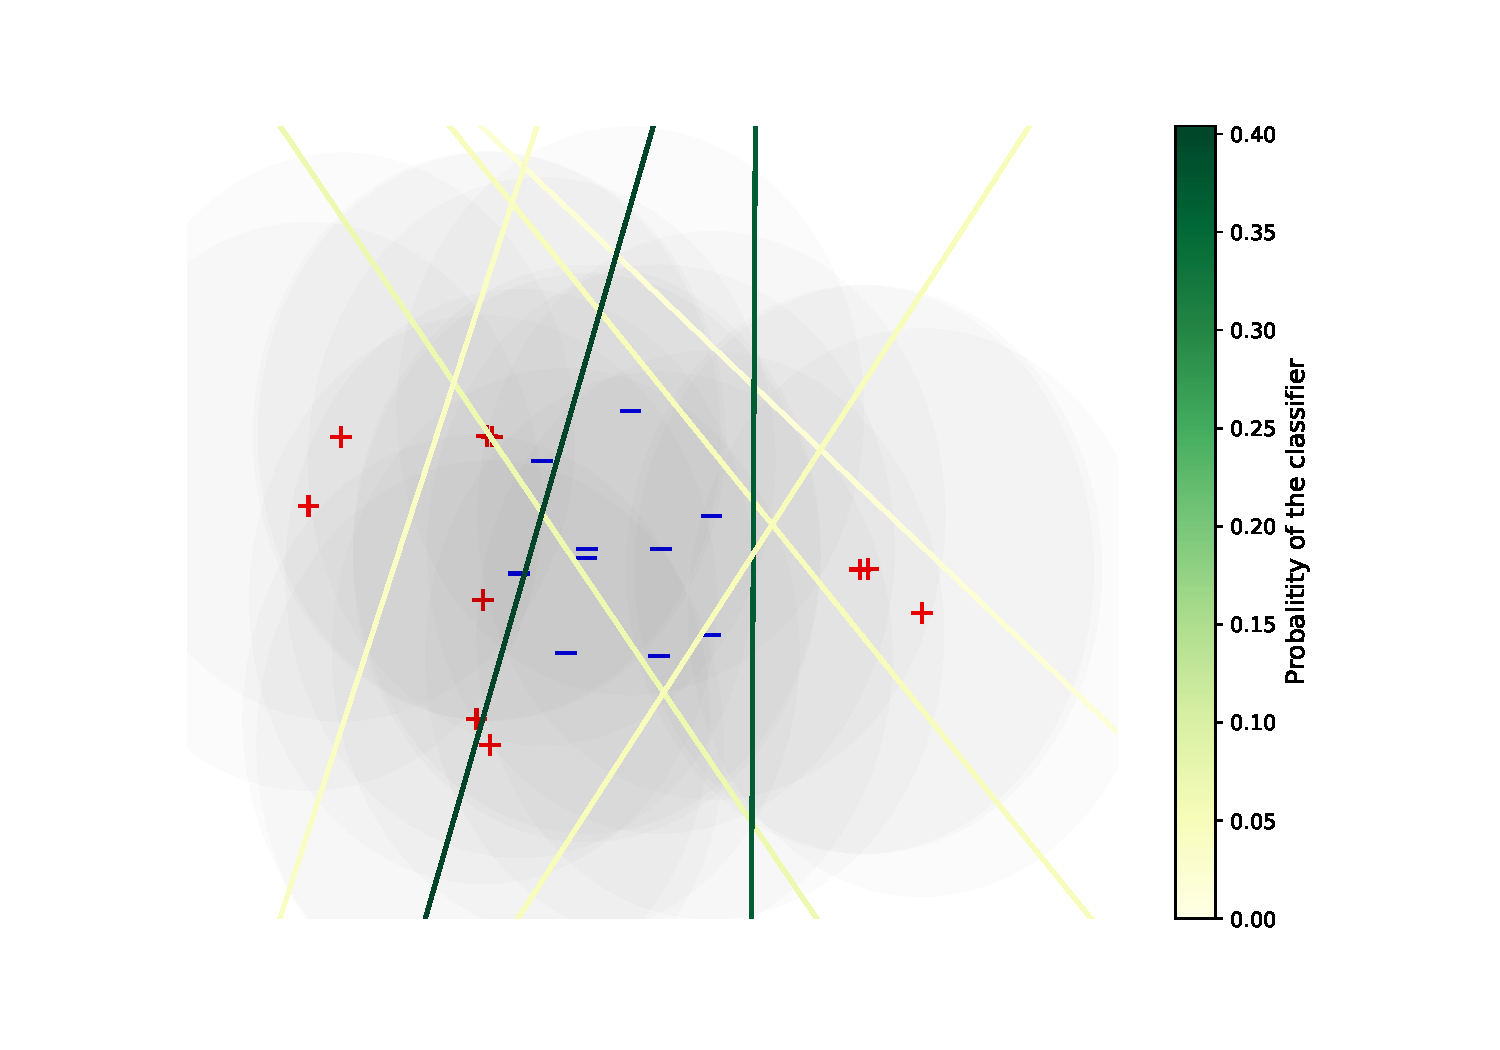
\includegraphics[width=0.32\textwidth]{Images/illustration.pdf}  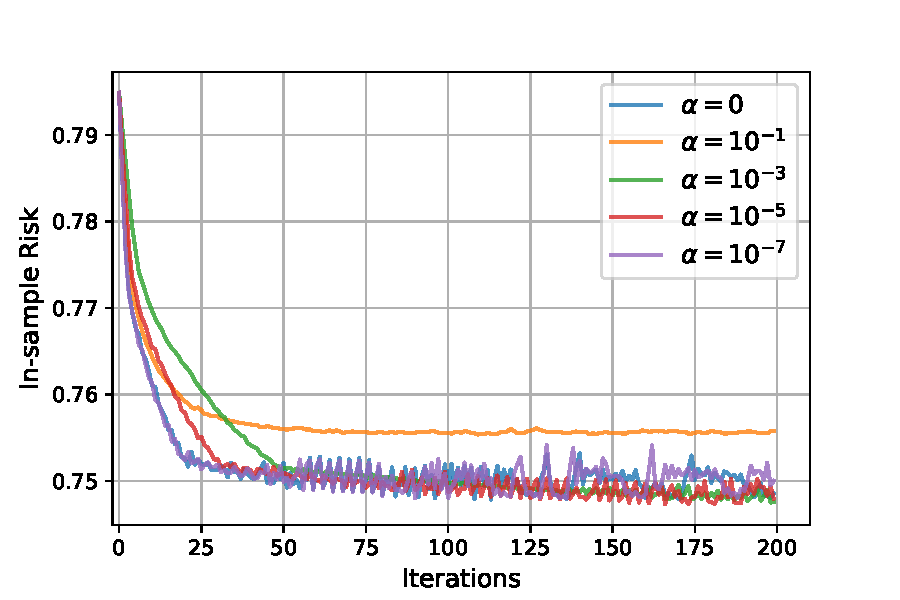
\includegraphics[width=0.32\textwidth]{Images/convergence_toy.pdf}     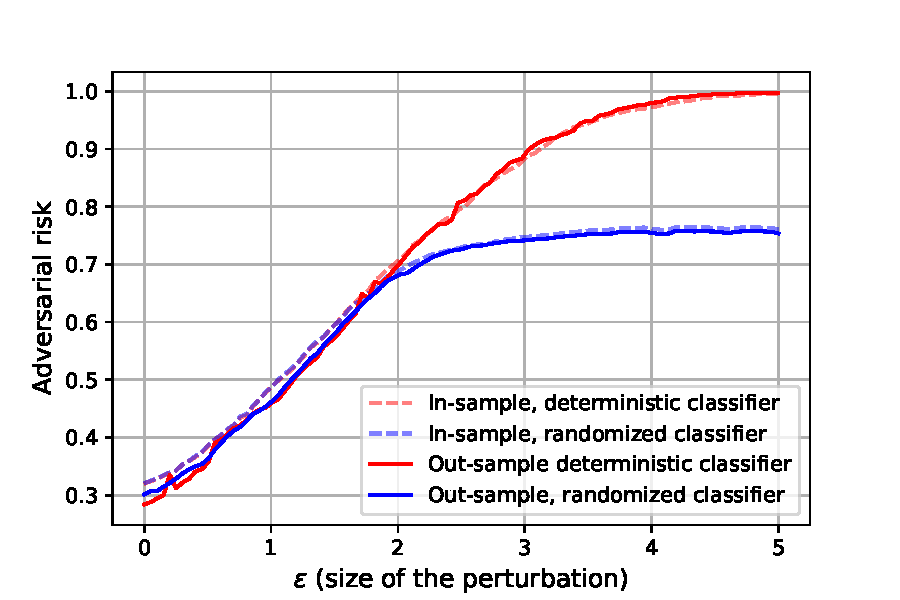
\includegraphics[width=0.32\textwidth]{Images/risk_toy.pdf}
    \caption{On left, $40$ data samples with their set of possible attacks represented in shadow and the optimal randomized classifier, with a color gradient representing the probability of the classifier. \textcolor{black}{In the middle}, convergence of the oracle ($\alpha=0$) and regularized algorithm for different values of regularization parameters. On right, in-sample and out-sample risk for randomized and deterministic minimum risk in function of the perturbation size $\varepsilon$. In the latter case, the randomized classifier is optimized with oracle Algorithm~\ref{algo:duchi}.}
    \label{fig:toy_example}
\end{figure*}


\textbf{An Entropic Relaxation.} Using the results from Section~\ref{sec:entropic-reg}, adding an entropic term to the objective allows to have a simple reformulation of the problem, as follows:
\begin{align*}
  \inf_{\bm{\lambda}\in \Delta_l}\sum_{i=1}^\numsamples  \frac{\varepsilon_i}{\numsamples}\log\left( \frac{1}{m_i}\sum_{j=1}^{m_i}\exp\left(\frac{\sum_{k=1}^l \lambda_k\loss(\theta_k,u_j^{(i)})}{\varepsilon_i}\right)\right)
\end{align*}
Note that in $\bm{\lambda}$, the objective is convex and smooth. One can  apply the accelerated PGD~\citep{beck2009fast,tseng2008accelerated} which enjoys an optimal convergence rate for first order methods of $\mathcal{O}(T^{-2})$ for $T$ iterations.

\textbf{A First Oracle Algorithm.} Indepedently from  the entropic regularization,we present an oracle-based algorithm inspired from~\citep{sinha2017certifying} and the convergence of projected sub-gradient methods~\citep{boyd2003subgradient}. The computation of the inner supremum problem is usually NP-hard. Let us justify it on a mixture of linear classifiers in binary classification: $f_{\theta_k,b_k}(x) = \langle \theta,x\rangle+b_k$ for $k\in [L]$ and $\bm{\lambda}=\mathbf{1}_L/L$. Let us consider the $\ell_2$ norm and $x=0$ and $y=1$. Then the problem of attacking $x$ is the following:
\begin{align*}
    \sup_{\tau,~\lVert \tau\rVert\leq\varepsilon} \frac{1}{L}\sum_{k=1}^L\mathbf{1}_{\langle \theta_k,x+\tau\rangle+b_k\leq0}
\end{align*}
This problem is equivalent to a linear binary classification problem on $\tau$, which is known to be NP-hard. Assuming the existence of a $\delta$-approximate oracle to this supremum, we algorithm is presented in Algorithm~\ref{algo:duchi}. We get the following guarantee for this algorithm. %See proof in Appendix~\ref{prv:algo-oracle}.
\begin{prop}
\label{prop:algo-oracle}
% Let $\PP\in\mathcal{M}^1_+(\mathcal{X}\times\mathcal{Y})$.
Let $\loss:\Theta\times(\mathcal{X}\times\mathcal{Y})\to [0,\infty)$ satisfying Assumption~\ref{ass:loss}. Then, Algorithm~\ref{algo:duchi} satisfies:  
\begin{align*}
    \min_{t\in[T]} \widehat{\mathcal{R}}_{adv}^{\varepsilon}(\bm{\lambda}_t)-\widehat{\mathcal{R}}_{adv}^{\varepsilon,*}\leq2\delta+\textcolor{black}{ \frac{2M\sqrt{l}}{\sqrt{T}}}
    % \delta\sqrt{K}+ \frac{M\sum_{t=1}^T \eta_t^2+\rVert\lambda_0-\lambda^*\lVert^2}{\sum_{t=1}^T\eta_t}
\end{align*}
% In particular for $\eta_t =\frac{\eta}{t^{1/2}}$, we get: $\min_{t\in[T]}\risk^\varepsilon(\lambda_t)-\risk^\varepsilon(\lambda^*)\in O\left(\delta+\frac{\log T}{\sqrt{T}}\right)$
\end{prop}

\begin{proof}
Thanks to Danskin theorem, if $\QQ^*$ is a best response to $\bm{\lambda}$, then $$\bm{g}^*:=\left(\mathbb{E}_{\QQ^*}\left[\loss(\theta_1,(x,y))\right],\dots,\mathbb{E}_{\QQ^*}\left[\loss(\theta_l,(x,y))\right]\right)^T$$ is a subgradient of $\bm{\lambda}\to \risk^\varepsilon(\bm{\lambda})$. Let $\eta\geq 0$ be the learning rate. Then we have for all $t\geq 1$:
\begin{align*}
\lVert \bm{\lambda}_t-\bm{\lambda}^*\rVert^2&\leq \lVert \bm{\lambda}_{t-1}-\eta \bm{g}_t-\bm{\lambda}^*\rVert^2\\
&=\lVert \bm{\lambda}_{t-1}-\bm{\lambda}^*\rVert^2-2\eta \langle\bm{g}_t, \bm{\lambda}_{t-1}-\bm{\lambda}^*\rangle+ \eta^2\lVert \bm{g}_t\rVert^2\\
&\leq \lVert \bm{\lambda}_{t-1}-\bm{\lambda}^*\rVert^2-2\eta \langle\bm{g}^*_t, \bm{\lambda}_{t-1}-\bm{\lambda}^*\rangle+2\eta\langle\bm{g}^*_t-\bm{g}_t, \bm{\lambda}_{t-1}-\bm{\lambda}^*\rangle+\eta^2 M^2 l\\
&\leq \lVert \bm{\lambda}_{t-1}-\bm{\lambda}^*\rVert^2-2\eta\left(\risk^\varepsilon(\bm{\lambda}_t)-\risk^\varepsilon(\bm{\lambda}^*)\right) +4\eta\delta+\eta^2  M^2 l%\lVert \bm{\lambda}_{t-1}-\bm{\lambda}^*\rVert_1
\end{align*}
We then deduce by summing:
\begin{align*}
   2\eta \sum_{t=1}^T \risk^\varepsilon(\bm{\lambda}_t)-\risk^\varepsilon(\bm{\lambda}^*) \leq 4\delta\eta T +\lVert \bm{\lambda}_{0}-\bm{\lambda}^*\rVert^2+\eta^2 M^2 lT
\end{align*}
Then we have:
\begin{align*}
    \min_{t\in[T]}\risk^\varepsilon(\bm{\lambda}_t)-\risk^\varepsilon(\bm{\lambda}^*)\leq 2\delta+\frac{4}{\eta T}+M^2l\eta
\end{align*}
The left-hand term is minimal for $\eta=\frac{2}{M\sqrt{lT}}$, and for this value:
\begin{align*}
    \min_{t\in[T]}\risk^\varepsilon(\bm{\lambda}_t)-\risk^\varepsilon(\bm{\lambda}^*)\leq 2\delta+\frac{2M\sqrt{l}}{\sqrt{T}}
\end{align*}
\end{proof}. 

The main drawback of the above algorithm is that one needs to have access to an oracle to guarantee the convergence of the proposed algorithm whereas its regularized version in order to approximate the solution and propose a simple algorithm to solve it.

 %In practice, we can change the distribution of sampling, to be more likely to find adversaries. 
% \begin{rmq}
% In general, one can use the exact same tools to obtain a proxy of the general DRO problem. Indeed thanks to~\citep{blanchet2019quantifying}, the dual can be approximated by adding an entropic term to the objective which leads to. We end-up with a minimization problem of a convex objective over the set of distribution. 
% \end{rmq}

\subsection{A General Heuristic Algorithm}

So far, our algorithms are not easily practicable in the case of deep learning. Adversarial examples are known to be easily transferrable from one model to another~\citep{tramer2017space,papernot2016transferability}. So we aim at learning diverse models. To this end, and support our theoretical claims, we propose an heuristic algorithm (see Algorithm~\ref{algo:heuristic}) to train a robust mixture of $l$ classifiers.   We alternatively train these classifiers with adversarial examples against the current mixture and update the probabilities of the mixture according to the algorithms we proposed in Section~\ref{sec:proposed-algo}. 


\begin{algorithm}[h!]
\SetAlgoLined
$l$: number of models, $T$: number of iterations,\\
$T_\theta$: number of updates for the models $\bm{\theta}$,\\
$T_\lambda$: number of updates for the mixture $\bm{\lambda}$,\\ $\bm{\lambda}_0=(\lambda_0^1,\dots\lambda_0^l),~\bm{\theta}_0=(\theta_0^1,\dots\theta_0^l)$\\
 \For{$t=1,\dots,T$}{
 Let $B_t$ be a batch of data.\\
\eIf{$t \mod (T_\theta l+1)\neq 0$}{
$k$ sampled uniformly in $\{1,\dots,l\}$\\
$\Tilde{B}_t\leftarrow$ Attack of images in $B_t$ for the  model $(\bm{\lambda}_t,\bm{\theta}_t)$\\
$\theta^t_k\leftarrow$ Update $\theta^{t-1}_k$ with $\Tilde{B}_t$ for fixed $\bm{\lambda}_t$ with a SGD step}{
$\bm{\lambda}_t\leftarrow$Update $\bm{\lambda}_{t-1}$ on $B_t$ for fixed $\bm{\theta}_t$
with oracle-based or regularized algorithm with $T_\lambda$ iterations.
}
  }
 \caption{Adversarial Training for Mixtures}
 
 \label{algo:heuristic}
\end{algorithm}


\section{Experiments}

\subsection{Synthetic Dataset}


To illustrate our theoretical findings, we start by testing our learning algorithm on the following synthetic two-dimensional problem. Let us consider the distribution $\PP$ defined as  $\PP\left(Y =\pm 1\right)=1/2$, $\PP\left(X\mid Y=-1\right) = \mathcal{N}(0,I_2)$ and $\PP\left(X \mid Y=1\right) = \frac12\left[\mathcal{N}((-3,0),I_2)+\mathcal{N}((3,0),I_2) \right]$.
% \begin{align*}
%   \left\{
%     \begin{array}{ll}
%   \\
%         \PP\left(X\mid Y=-1\right) = \mathcal{N}(0,I_2) \\
%         \PP\left(X \mid Y=1\right) = \frac12\left[\mathcal{N}((-3,0),I_2)+\mathcal{N}((3,0),I_2) \right].
%     \end{array}
% \right. 
% \end{align*}
We sample $1000$ training points from this distribution and randomly generate $10$ linear classifiers that achieves a standard training risk lower than $0.4$. To simulate an adversary with budget $\varepsilon$ in $\ell_2$ norm, we proceed as follows. For every sample $(x,y)\sim \PP$ we generate $1000$ points uniformly at random in the ball of radius $\varepsilon$ and select the one maximizing the risk for the $0/1$ loss. Figure~\ref{fig:toy_example} (left) illustrates the type of mixture we get after convergence of our algorithms. Note that in this toy problem, we are likely to find the optimal adversary with this sampling strategy if we sample enough attack points. 
% \begin{figure}[ht]
%     \centering
%     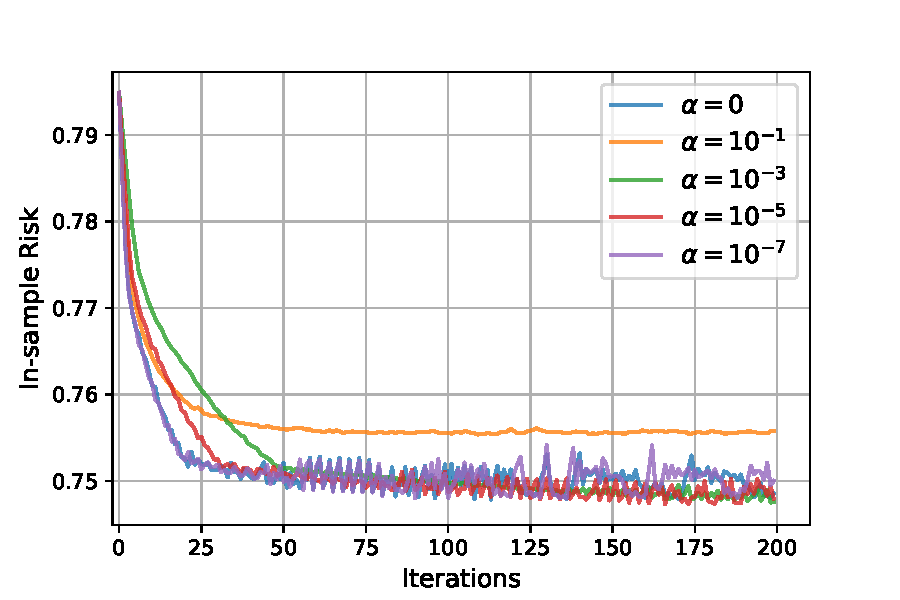
\includegraphics[width=0.46\textwidth]{Images/convergence_toy.pdf}
%     \caption{Caption}
%     \label{fig:toy_example_cvgence}
% \end{figure}
\begin{figure*}[!ht]
\begin{center}

\textbf{Adversarial Training, CIFAR-10 dataset results}
 \begin{small}
\begin{tabular}{c|c|ccc} 
\textbf{ Models} & \textbf{Acc. }&\textbf{$\textrm{APGD}_\textrm{CE}$}& \textbf{$\textrm{APGD}_\textrm{DLR}$} & \textbf{Rob. Acc.} \\ \hline
 1 & $81.9\%$ &	$47.6\%$ & $47.7\%$ & $45.6\%$ \\ 
 2 & $81.9\%$ & $49.0\%$ & ${49.6\%}$ & ${47.0\%}$\\ 
  3 & ${81.7\%}$& ${49.0\%}$ & $49.3\%$ & ${46.9\%}$\\
    4 & $\bm{82.6\%}$& $\bm{49.7\%}$ & $\bm{49.8}\%$ & $\bm{47.2\%}$\\

\end{tabular}
\end{small}\\
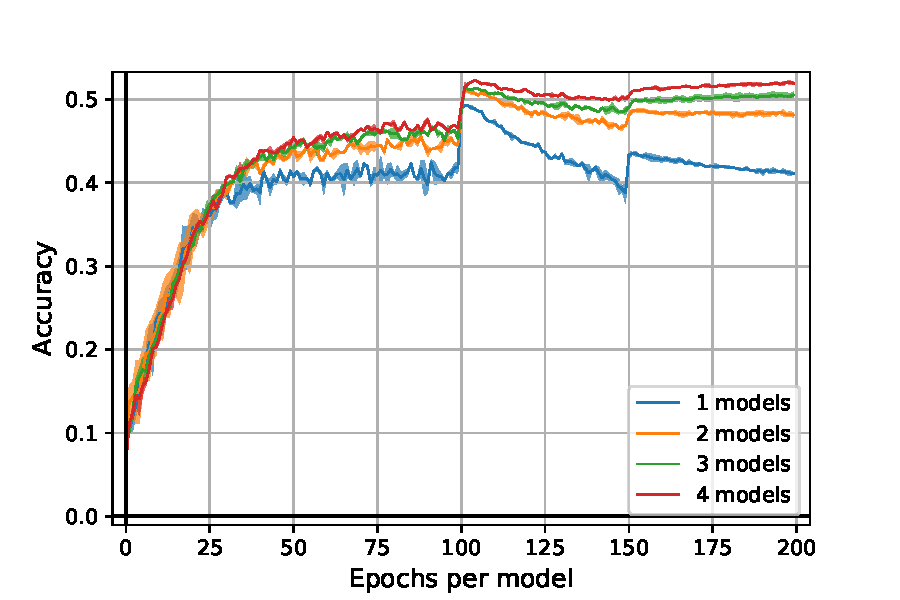
\includegraphics[width=0.35\textwidth]{Images/robust_acc_finalrun_ResNet18_1024_200_0.001.pdf}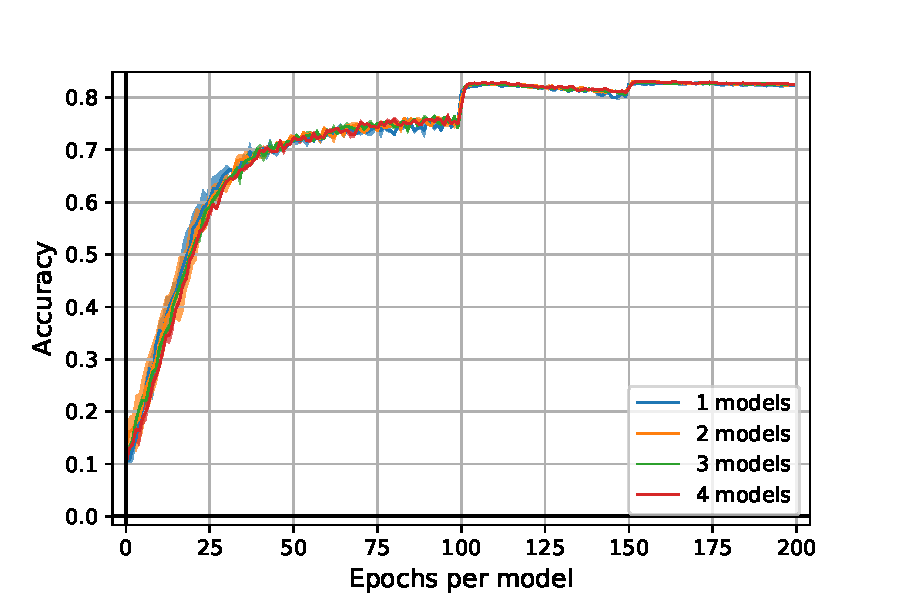
\includegraphics[width=0.35\textwidth]{Images/standard_acc_finalrun_ResNet18_1024_200_0.001.pdf} 
  

\textbf{TRADES, CIFAR-10 dataset results}

 \begin{small}
\begin{tabular}{c|c|ccc} 
\textbf{ Models} & \textbf{Acc. }&\textbf{$\textrm{APGD}_\textrm{CE}$}& \textbf{$\textrm{APGD}_\textrm{DLR}$} & \textbf{Rob. Acc.} \\ \hline
 1 &  $79.6\%$ &$50.9\%$& $48.9\%$ &$48.3\%$ \\ 
 2 & $80.3\%$& $52.3\%$ &$51.2\%$ &$50.2\%$\\ 
  3 & $80.7\%$& $52.8\%$ &$51.7\%$ &$50.7\%$\\
    4 & \bm{$80.9\%$} & \bm{$53.0\%$}& \bm{$51.8\%$}& \bm{$50.8\%$}\\

\end{tabular}
\end{small}

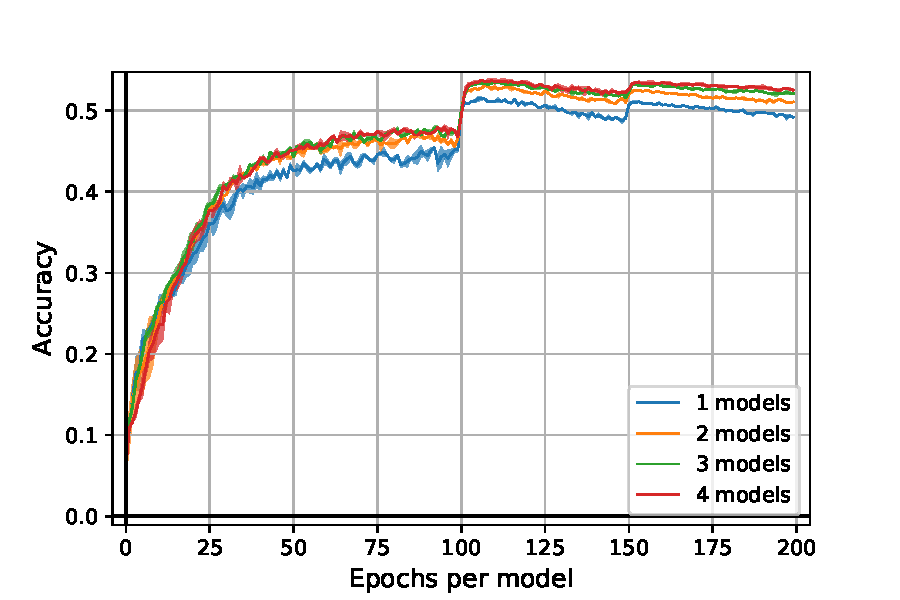
\includegraphics[width=0.35\textwidth]{Images/robust_acc_CIFAR10_final_cam_ready_bisss_ResNet18_1024_200_0.001.pdf}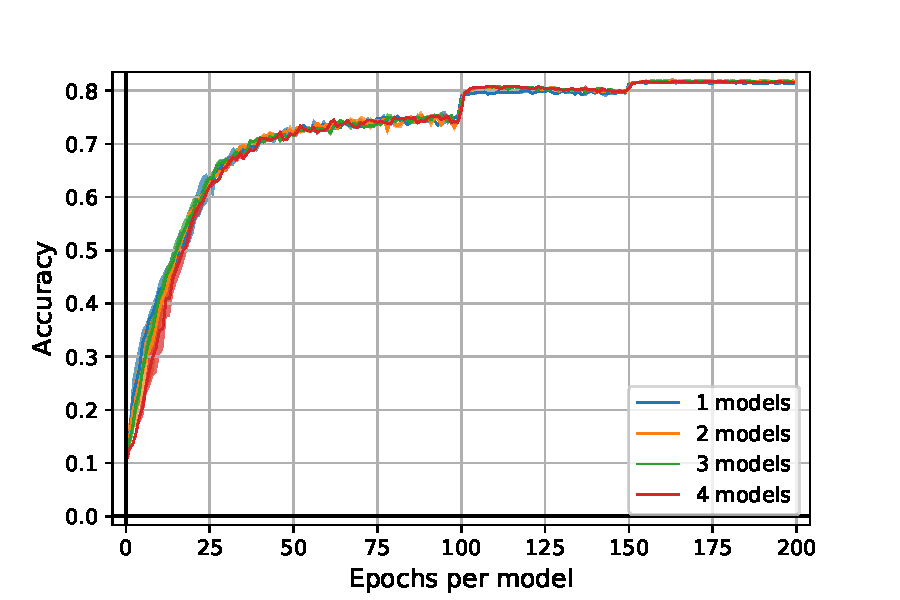
\includegraphics[width=0.35\textwidth]{Images/standard_acc_CIFAR10_final_cam_ready_bisss_ResNet18_1024_200_0.001.pdf} 
  

\textbf{Adversarial Training, CIFAR-100 dataset results}
 \begin{small}
\begin{tabular}{c|c|ccc} 
\textbf{ Models} & \textbf{Acc. }&\textbf{$\textrm{APGD}_\textrm{CE}$}& \textbf{$\textrm{APGD}_\textrm{DLR}$} & \textbf{Rob. Acc.} \\ \hline
 1 & $55.2\%$& $24.1\%$& $23.8\%$ & $22.5\%$\\ 
 2 & $55.2\%$ & $25.3\%$ &$26.1\%$ &$23.6\%$\\ 
  3 & \bm{$55.4\%$} & $25.7\%$ &$26.8\%$ &$24.2\%$\\
    4 & $55.3\%$ & \bm{$26.0\%$} & \bm{$27.5\%$}& \bm{$24.5\%$}\\

\end{tabular}
\end{small}
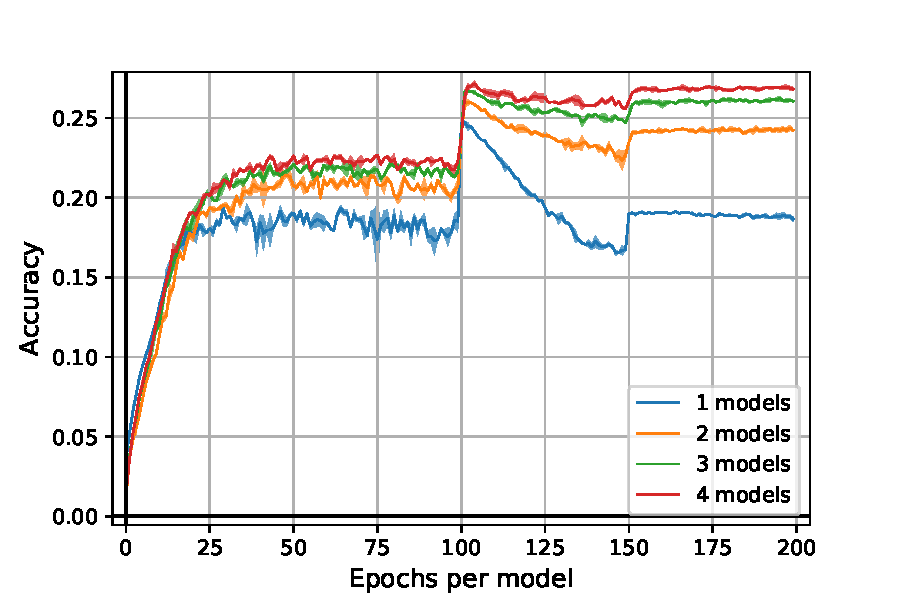
\includegraphics[width=0.35\textwidth]{Images/robust_acc_CIFAR100_finalrun_ResNet18_1024_200_0.001.pdf}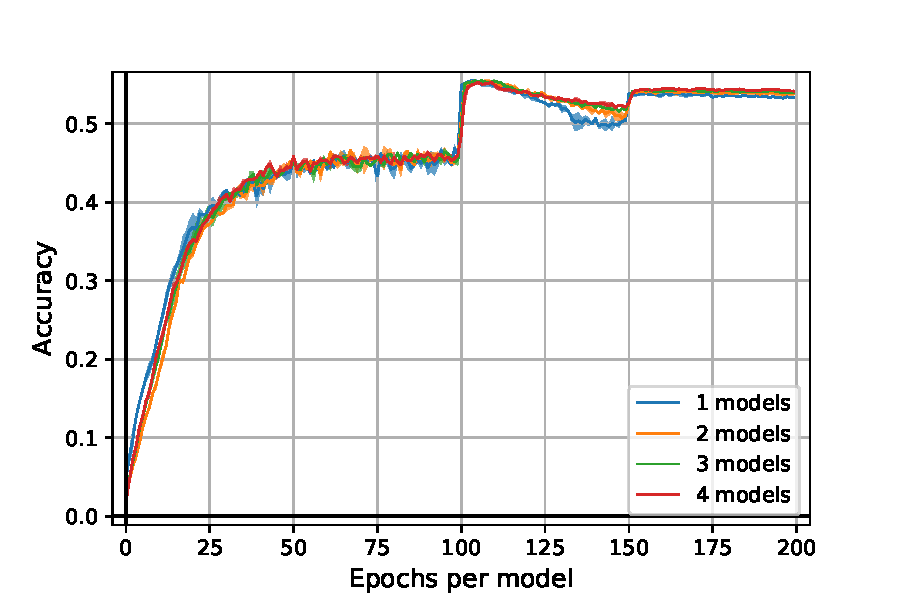
\includegraphics[width=0.35\textwidth]{Images/standard_acc_CIFAR100_finalrun_ResNet18_1024_200_0.001.pdf} 


 \caption{Upper plots: Adversarial Training, CIFAR-10 dataset results. Middle plots:  TRADES, CIFAR-10 dataset results. Bottom plots: CIFAR-100 dataset results. {On left}: Comparison of our algorithm with a standard adversarial training (one model). We reported the results for the model with the best robust accuracy obtained over two independent runs because adversarial training might be unstable. Standard and Robust accuracy (respectively in the middle and on right) on CIFAR-10 test images in function of the number of epochs per classifier with $1$ to $3$ ResNet18 models. The performed attack is PGD with $20$ iterations and $\varepsilon=8/255$.}
\label{fig:results_cifar}

\end{center}
\end{figure*}

To evaluate the convergence of our algorithms, we compute the adversarial risk of our mixture for each iteration of both the oracle and regularized algorithms. Figure~\ref{fig:toy_example} illustrates the convergence of the algorithms w.r.t the regularization parameter. We observe that the risk for both algorithms converge. Moreover, they converge towards the oracle minimizer when the regularization parameter $\alpha$ goes to $0$.

Finally, to demonstrate the improvement randomized techniques offer against deterministic defenses, we plot in Figure~\ref{fig:toy_example} (right) the minimum adversarial risk for both randomized and deterministic classifiers w.r.t. $\varepsilon$. The adversarial risk is strictly better for randomized classifier whenever the adversarial budget $\varepsilon$ is bigger than $2$. This illustration validates our analysis of Theorem~\ref{thm:duality-rand}, and motivates a in depth study of a more challenging framework, namely image classification with neural networks.

% \begin{figure}[ht]
%     \centering
%     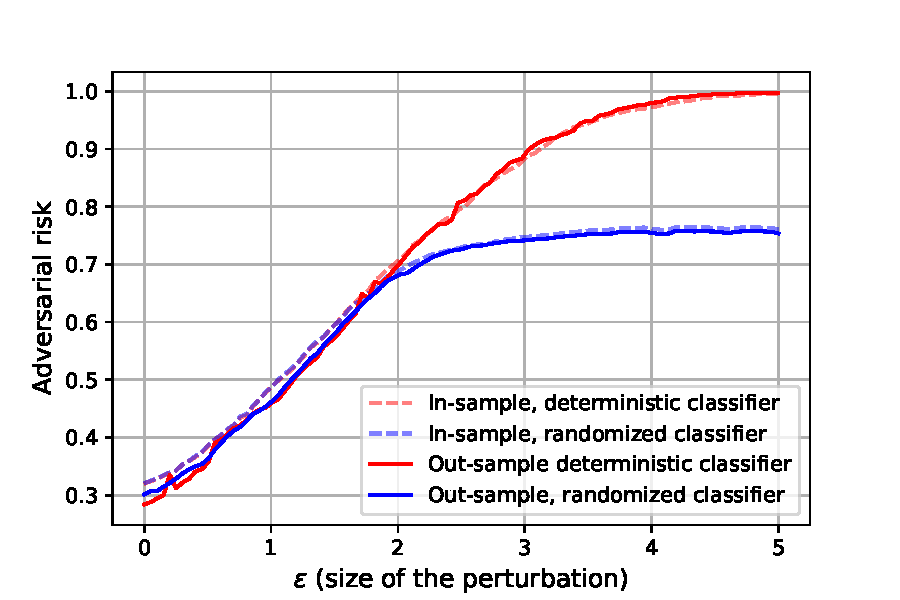
\includegraphics[width=0.46\textwidth]{Images/risk_toy.pdf}
%     \caption{Caption}
%     \label{fig:toy_example_risk}
% \end{figure}

\subsection{CIFAR Datasets}

% \begin{figure*}[!ht]
% \begin{center}

% \vskip 0.15in
%  \begin{minipage}[ht!]{0.39\textwidth}
%  \begin{scriptsize}
% \begin{tabular}{c|c|ccc} 
% \textbf{ Models} & \textbf{Acc. }&\textbf{$\textrm{APGD}_\textrm{CE}$}& \textbf{$\textrm{APGD}_\textrm{DLR}$} & \textbf{Rob. Acc.} \\ \hline
%  1 & $81.9\%$ &	$47.6\%$ & $47.7\%$ & $45.6\%$ \\ 
%  2 & $81.9\%$ & $49.0\%$ & ${49.6\%}$ & ${47.0\%}$\\ 
%   3 & ${81.7\%}$& ${49.0\%}$ & $49.3\%$ & ${46.9\%}$\\
%     4 & $\bm{82.6\%}$& $\bm{49.7\%}$ & $\bm{49.8}\%$ & $\bm{47.2\%}$\\

% \end{tabular}
% \end{scriptsize}
%   \end{minipage}\begin{minipage}[!ht]{0.61\textwidth}
% 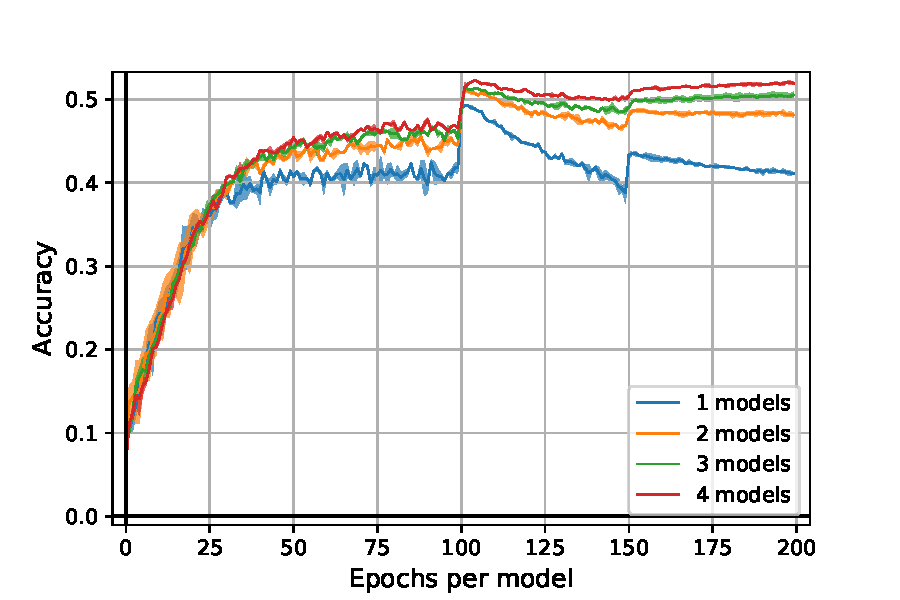
\includegraphics[width=0.49\textwidth]{Images/robust_acc_finalrun_ResNet18_1024_200_0.001.pdf}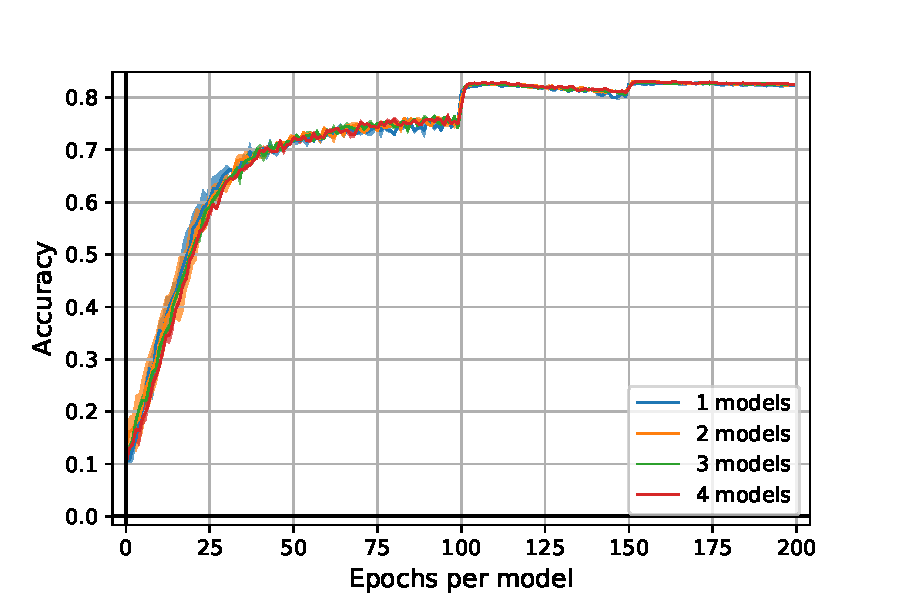
\includegraphics[width=0.49\textwidth]{Images/standard_acc_finalrun_ResNet18_1024_200_0.001.pdf} 
%   \end{minipage}
  
% Adversarial Training, CIFAR-10 dataset results

% \vskip 0.15in
%  \begin{minipage}[ht!]{0.39\textwidth}
%  \begin{scriptsize}
% \begin{tabular}{c|c|ccc} 
% \textbf{ Models} & \textbf{Acc. }&\textbf{$\textrm{APGD}_\textrm{CE}$}& \textbf{$\textrm{APGD}_\textrm{DLR}$} & \textbf{Rob. Acc.} \\ \hline
%  1 &  $79.6\%$ &$50.9\%$& $48.9\%$ &$48.3\%$ \\ 
%  2 & $80.3\%$& $52.3\%$ &$51.2\%$ &$50.2\%$\\ 
%   3 & $80.7\%$& $52.8\%$ &$51.7\%$ &$50.7\%$\\
%     4 & \bm{$80.9\%$} & \bm{$53.0\%$}& \bm{$51.8\%$}& \bm{$50.8\%$}\\

% \end{tabular}
% \end{scriptsize}
%   \end{minipage}\begin{minipage}[!ht]{0.61\textwidth}
% 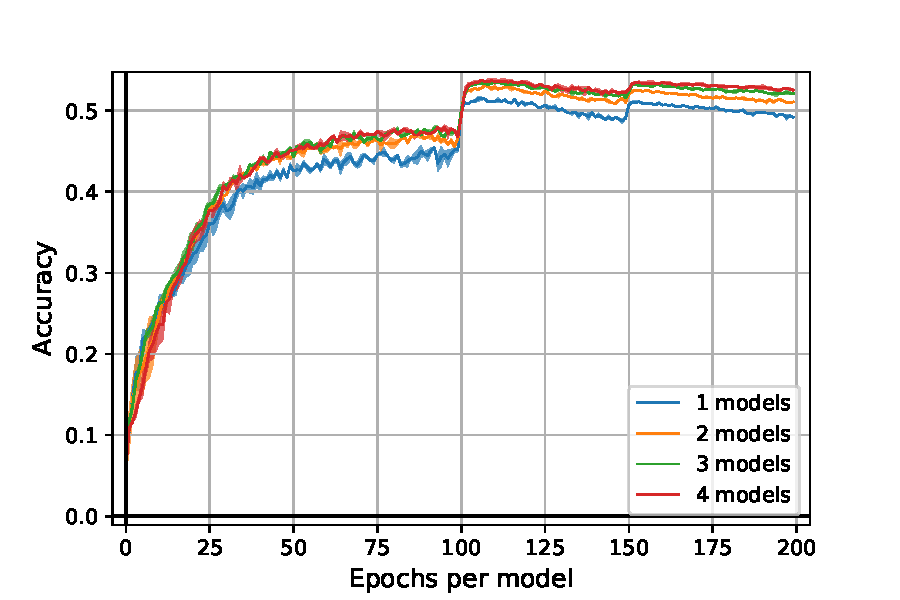
\includegraphics[width=0.49\textwidth]{Images/robust_acc_CIFAR10_final_cam_ready_bisss_ResNet18_1024_200_0.001.pdf}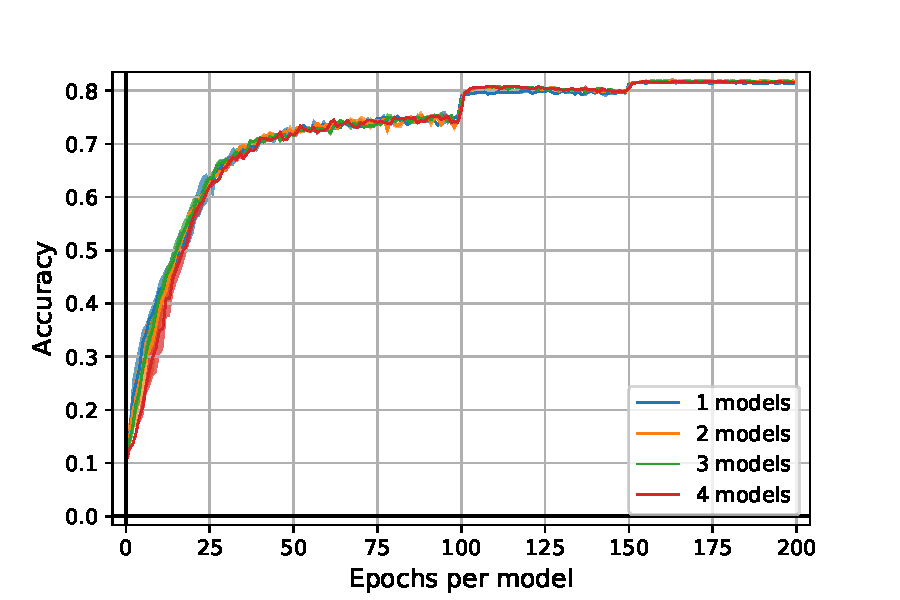
\includegraphics[width=0.49\textwidth]{Images/standard_acc_CIFAR10_final_cam_ready_bisss_ResNet18_1024_200_0.001.pdf} 
%   \end{minipage}
  
% TRADES, CIFAR-10 dataset results
% \vskip 0.15in
%  \begin{minipage}[ht!]{0.39\textwidth}
%  \begin{scriptsize}
% \begin{tabular}{c|c|ccc} 
% \textbf{ Models} & \textbf{Acc. }&\textbf{$\textrm{APGD}_\textrm{CE}$}& \textbf{$\textrm{APGD}_\textrm{DLR}$} & \textbf{Rob. Acc.} \\ \hline
%  1 & $55.2\%$& $24.1\%$& $23.8\%$ & $22.5\%$\\ 
%  2 & $55.2\%$ & $25.3\%$ &$26.1\%$ &$23.6\%$\\ 
%   3 & \bm{$55.4\%$} & $25.7\%$ &$26.8\%$ &$24.2\%$\\
%     4 & $55.3\%$ & \bm{$26.0\%$} & \bm{$27.5\%$}& \bm{$24.5\%$}\\

% \end{tabular}
% \end{scriptsize}
%   \end{minipage}\begin{minipage}[!ht]{0.61\textwidth}
% 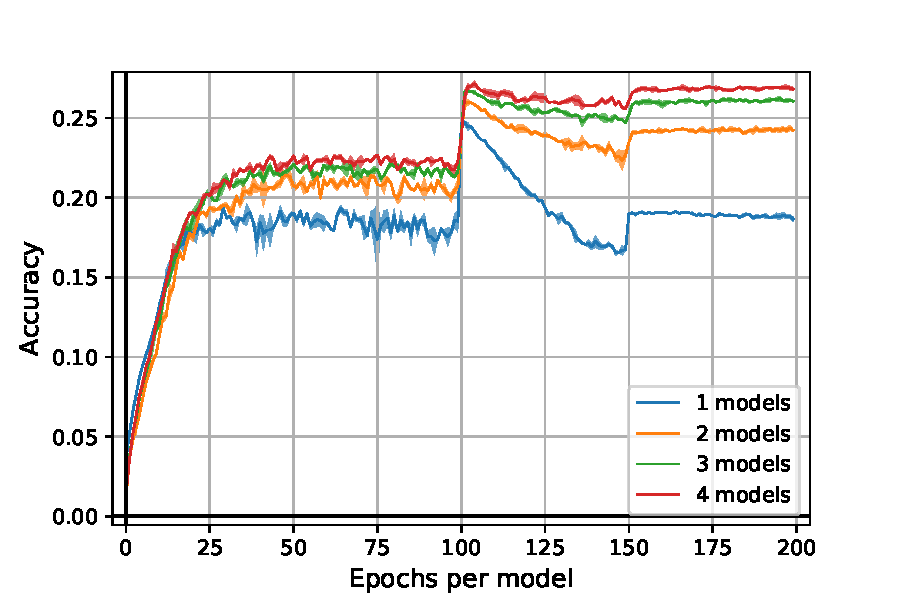
\includegraphics[width=0.49\textwidth]{Images/robust_acc_CIFAR100_finalrun_ResNet18_1024_200_0.001.pdf}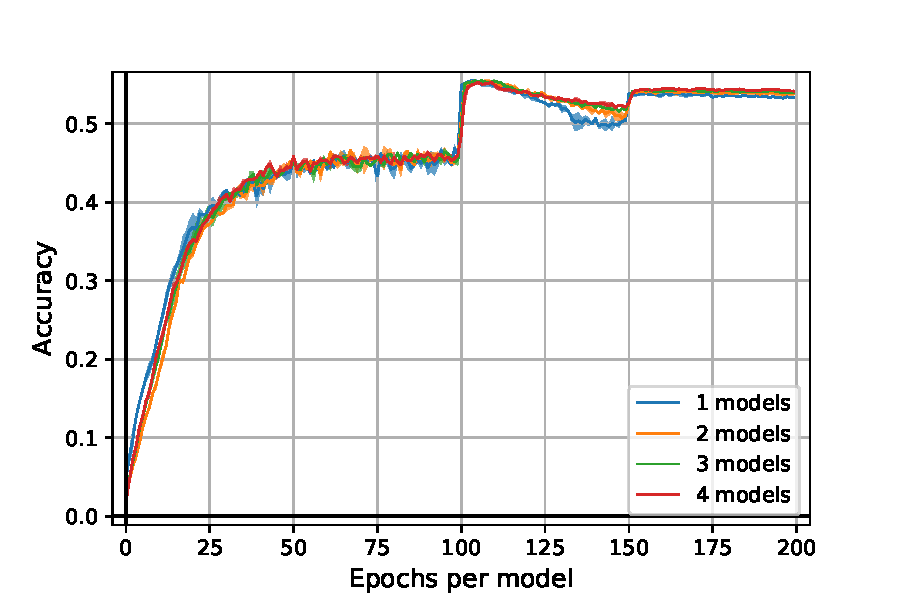
\includegraphics[width=0.49\textwidth]{Images/standard_acc_CIFAR100_finalrun_ResNet18_1024_200_0.001.pdf} 
%   \end{minipage}
%   Adversarial Training, CIFAR-100 dataset results

%  \caption{Upper plots: Adversarial Training, CIFAR-10 dataset results. Middle plots:  TRADES, CIFAR-10 dataset results. Bottom plots: CIFAR-100 dataset results. {On left}: Comparison of our algorithm with a standard adversarial training (one model). We reported the results for the model with the best robust accuracy obtained over two independent runs because adversarial training might be unstable. Standard and Robust accuracy (respectively in the middle and on right) on CIFAR-10 test images in function of the number of epochs per classifier with $1$ to $3$ ResNet18 models. The performed attack is PGD with $20$ iterations and $\varepsilon=8/255$.}
% \label{fig:results_cifar}

% \end{center}
% \end{figure*}

% Adversarial examples are known to be easily transferrable from one model to another~\cite{tramer2017space}. To counter this and support our theoretical claims, we propose an heuristic algorithm (see Algorithm~\ref{algo:heuristic}) to train a robust mixture of $L$ classifiers. We alternatively train these classifiers with adversarial examples against the current mixture and update the probabilities of the mixture according to the algorithms we proposed in Section~\ref{sec:proposed-algo}. More details on the heuristic algorithm are available in Appendix~\ref{sec:additional-xp}. 
% \begin{algorithm}[h!]
% \small
% \SetAlgoLined
% $L$: number of models, $T$: number of iterations,\\
% $T_\theta$: number of updates for the models $\bm{\theta}$,\\
% $T_\lambda$: number of updates for the mixture $\bm{\lambda}$,\\ $\bm{\lambda}_0=(\lambda_0^1,\dots\lambda_0^L),~\bm{\theta}_0=(\theta_0^1,\dots\theta_0^L)$\\
%  \For{$t=1,\dots,T$}{
%  Let $B_t$ be a batch of data.\\
% \eIf{$t \mod (T_\theta L+1)\neq 0$}{
% $k$ sampled uniformly in $\{1,\dots,L\}$\\
% $\Tilde{B}_t\leftarrow$ Attack of images in $B_t$ for the  model $(\bm{\lambda}_t,\bm{\theta}_t)$\\
% $\theta^t_k\leftarrow$ Update $\theta^{t-1}_k$ with $\Tilde{B}_t$ for fixed $\bm{\lambda}_t$ with a SGD step}{
% $\bm{\lambda}_t\leftarrow$Update $\bm{\lambda}_{t-1}$ on $B_t$ for fixed $\bm{\theta}_t$
% with oracle or regularized algorithm with $T_\lambda$ iterations.
% }
%   }
%  \caption{Adversarial Training for Mixtures}
 
%  \label{algo:heuristic}
% \end{algorithm}

\paragraph{Experimental Setup.} We now implement our heuristic algorithm (Alg.~\ref{algo:heuristic}) on CIFAR-10 and CIFAR-100 datasets for both Adversarial Traning~\citep{madry2017towards} and TRADES~\citep{zhang2019theoretically} loss. To evaluate the performance of Algorithm~\ref{algo:heuristic}, we trained from $1$ to $4$ ResNet18~\citep{He_2016_CVPR} models on $200$ epochs per model\footnote{$L\times200$ epochs in total, where $L$ is the number of models.}. We study the robustness with regards to $\ell_\infty$ norm and fixed adversarial budget $\varepsilon=8/255$. The attack we used in the inner maximization of the training is an adapted (adaptative) version of PGD for mixtures of classifiers with $10$ steps. Note that for one single model, Algorithm~\ref{algo:heuristic} exactly corresponds to adversarial training~\citep{madry2017towards} or TRADES. For each of our setups, we made two independent runs and select the  best one. The training time of our algorithm is around four times longer than a standard Adversarial Training (with PGD 10 iter.) with two models, eight times with three models and twelve times with four models. We trained our models with a batch of size  $1024$ on $8$ Nvidia V100 GPUs. 

\paragraph{Optimizer.} For each of our models, The optimizer we used in all our implementations is SGD with learning rate set to $0.4$ at epoch $0$ and is divided by $10$ at half training then by $10$ at the three quarters of training. The momentum is set to $0.9$ and the weight decay to $5\times10^{-4}$. The batch size is set to $1024$. 
\paragraph{Adaptation of Attacks.} Since our classifier is randomized, we need to adapt the attack accordingly. To do so we used the expected loss:
\begin{align*}
\Tilde{\loss}\left((\bm{\lambda},\bm{\theta}),(x,y)\right) = \sum_{k=1}^L \lambda_k \loss(\theta_k,(x,y))
\end{align*}
to compute the gradient in the attacks, regardless the loss (DLR or cross-entropy). For the inner maximization at training time, we used a PGD attack on the cross-entropy loss with $\varepsilon=0.03$. For the final evaluation, we used the untargeted $DLR$ attack with default parameters.
\paragraph{Regularization in Practice.} The entropic regularization in higher dimensional setting need to be adapted to be more likely to find adversaries. To do so, we computed PGD attacks with only $3$ iterations with $5$ different restarts instead of sampling uniformly $5$ points  in the $\ell_\infty$-ball. In our experiments in the main paper, we use a regularization parameter $\alpha=0.001$. The learning rate for the minimization on $\bm{\lambda}$ is always fixed to $0.001$. 
\paragraph{Alternate Minimization Parameters.} Algorithm~\ref{algo:heuristic} implies an alternate minimization algorithm. We set the number of updates of $\bm{\theta}$ to $T_\theta = 50$ and, the update of $\bm{\lambda}$ to $T_\lambda = 25$. 

\subsection{Effect of the Regularization}
In this subsection, we experimentally investigate the effect of the regularization. In Figure~\ref{fig:xp-regularization}, we notice, that the regularization has the effect of stabilizing, reducing the variance and improving the level of the robust accuracy for adversarial training for mixtures (Algorithm~\ref{algo:heuristic}). The standard accuracy curves are very similar in both cases.



\paragraph{Evaluation Protocol.} At each epoch, we evaluate the current mixture on test data against PGD attack  with $20$ iterations. To select our model and avoid overfitting~\citep{rice2020overfitting}, we kept the most robust against this PGD attack.
To make a final evaluation of our mixture of models, we used an adapted version of $\textrm{AutoPGD}$ untargeted attacks~\citep{croce2020reliable} for randomized classifiers with both Cross-Entropy (CE) and Difference of Logits Ratio (DLR) loss. For both attacks, we made $100$ iterations and $5$ restarts.

\paragraph{Results.} The results are presented in Figure~\ref{fig:results_cifar}. We remark our algorithm outperforms a standard adversarial training in all the cases by more $1\%$ on CIFAR-10 and CIFAR-100, without additional loss of standard accuracy as it is attested by the left figures. On TRADES, the gain is even more important by more than $2\%$ in robust accuracy. Moreover, it seems our algorithm, by adding more and more models, reduces the overfitting of adversarial training. It also appears that robustness increases as the number of models increases. So far, experiments are computationally very costful and it is difficult to raise precise conclusions. Further, hyperparameter tuning ~\citep{gowal2020uncovering} such as architecture, unlabeled data~\citep{carmon2019unlabeled} or activation function may still increase the results.





% \begin{figure*}[!ht]
% \begin{center}


% \label{table:results}
% \vskip 0.15in
%  \begin{minipage}[!ht]{0.39\textwidth}
%  \begin{scriptsize}
% \begin{tabular}{c|c|ccc} 
% \textbf{ Models} & \textbf{Acc. }&\textbf{$\textrm{APGD}_\textrm{CE}$}& \textbf{$\textrm{APGD}_\textrm{DLR}$} & \textbf{Rob. Acc.} \\ \hline
%  1 & $81.9\%$ &	$47.6\%$ & $47.7\%$ & $45.6\%$ \\ 
%  2 & $81.9\%$ & $49.0\%$ & ${49.6\%}$ & ${47.0\%}$\\ 
%   3 & ${81.7\%}$& ${49.0\%}$ & $49.3\%$ & ${46.9\%}$\\
%     4 & $\bm{82.6\%}$& $\bm{49.7\%}$ & $\bm{49.8}\%$ & $\bm{47.2\%}$\\

% \end{tabular}
% \end{scriptsize}
%   \end{minipage}\begin{minipage}[!ht]{0.61\textwidth}
% 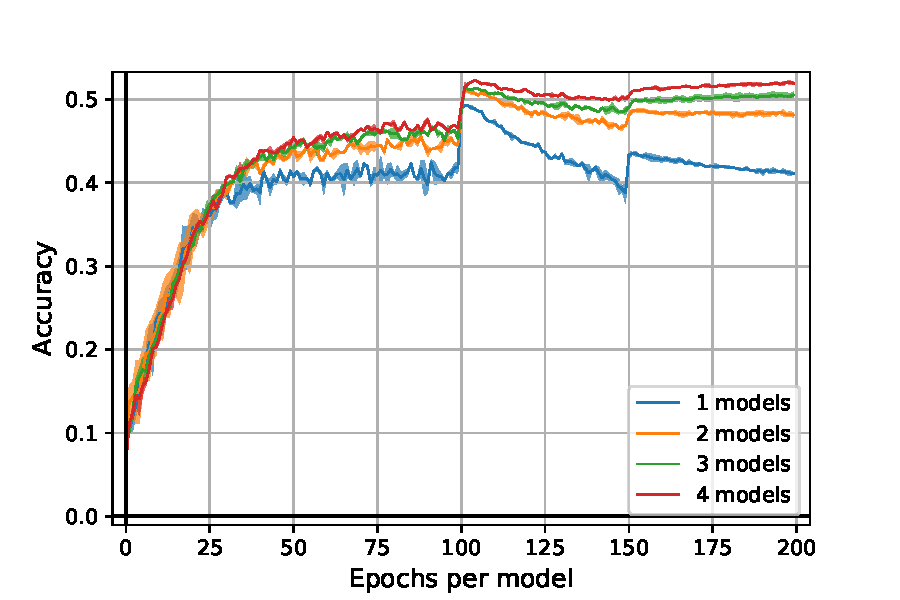
\includegraphics[width=0.49\textwidth]{Images/robust_acc_finalrun_ResNet18_1024_200_0.001.pdf}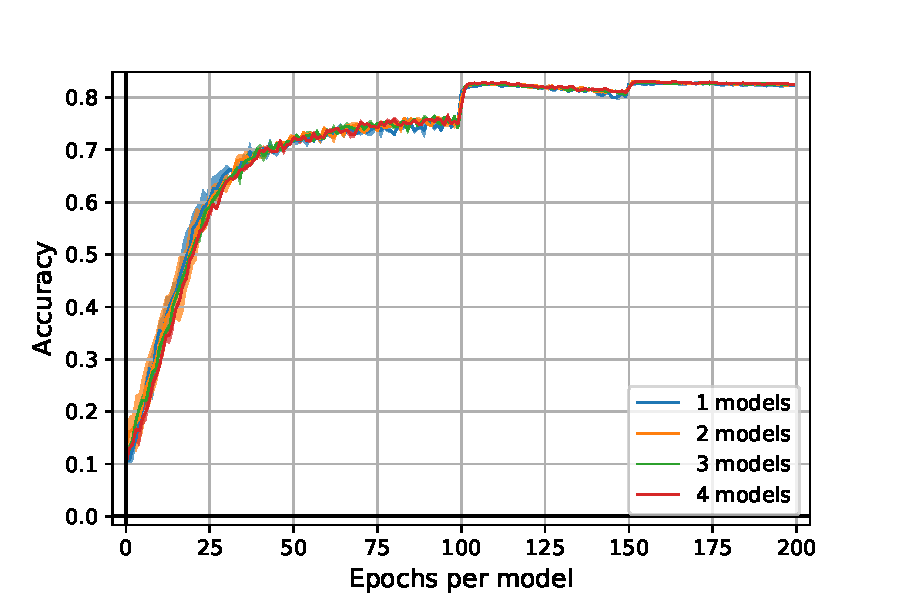
\includegraphics[width=0.49\textwidth]{Images/standard_acc_finalrun_ResNet18_1024_200_0.001.pdf} 
%   \end{minipage}
  
% \caption{On left: Comparison of our algorithm with a standard adversarial training (one model). We reported the results for the model with the best robust accuracy obtained over two independent runs because adversarial training might be unstable. Standard and Robust accuracy ( respectively in the center and on left) on CIFAR-10 test images in function of the number of epochs per classifier with $1$ to $3$ ResNet18 models. The performed attack is PGD with $20$ iterations and $\varepsilon=8/255$.}
% \label{fig:results_cifar}
% \end{center}
% \end{figure*}











% \begin{figure}[!ht]
% 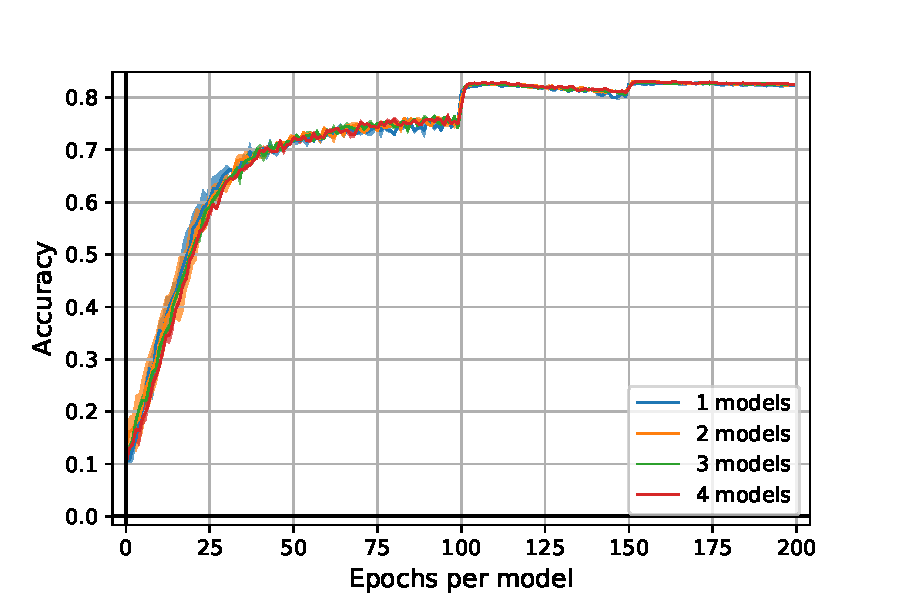
\includegraphics[width=0.46\textwidth]{Images/standard_acc_finalrun_ResNet18_1024_200_0.001.pdf}    \caption{Standard accuracy on CIFAR-10 test images in function of the number of epochs per classifier with $1$ to $3$ ResNet18 models.}
%     \label{fig:plot_standard_acc}
% \end{figure}

% \begin{figure}[!ht]
% 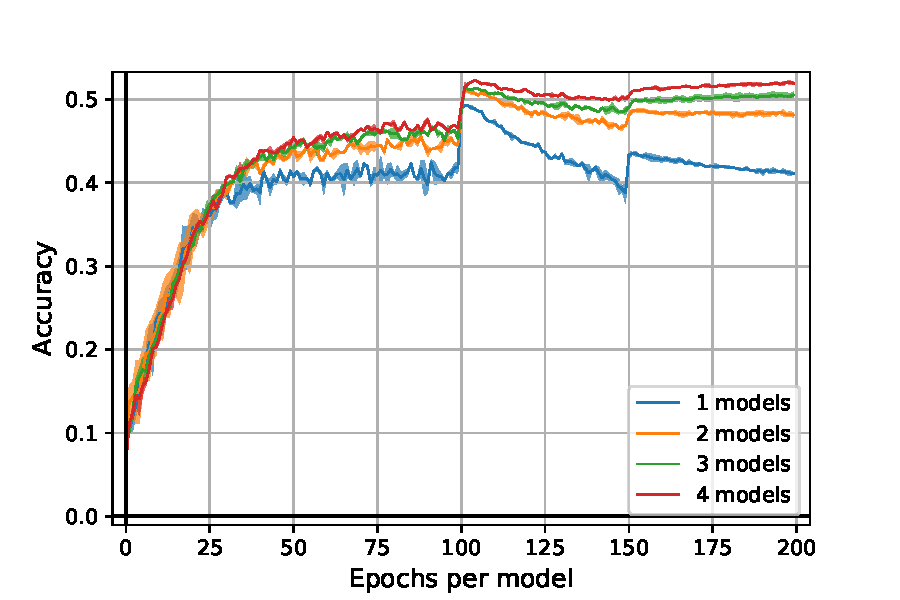
\includegraphics[width=0.46\textwidth]{Images/robust_acc_finalrun_ResNet18_1024_200_0.001.pdf}    \caption{Robust accuracy on CIFAR-10 test images in function of the number of epochs per classifier with $1$ to $3$ ResNet18 models. The attack performed is PGD with $20$ iterations and $\varepsilon=8/255$.}
%     \label{fig:plot_robust_acc}
% \end{figure}



% mettre ca au propre mais les resultats sont la!!

% setup: ResNet18 ou WRN28x10

% Details in supmat: loss +lr + format of training etc

% In supmat: 
% \begin{enumerate}
%     \item details HP (attack + training)
%     \item details runtime
%     \item additional results (with other attacks maybe + other archis...)
    
    
% \end{enumerate}
% Epochs 100

\section{Additional Lemmas and Results for Chapter~\ref{chap:game}}
% \subsection{Useful Lemmas}
% \begin{lemma}[Fubini's theorem]
% \label{lem:fubini}
% Let $l:\Theta\times(\mathcal{X}\times\mathcal{Y})\rightarrow [0,\infty)$ satisfying Assumption~\ref{ass:loss}. Then for all $\mu\in\mathcal{M}^1_+(\Theta)$, $\int l(\theta,\cdot)d\mu(\theta)$ is Borel measurable; for  $\QQ\in\mathcal{M}^1_+(\mathcal{X}\times\mathcal{Y})$, $\int l(\cdot,(x,y))d\QQ(x,y)$ is Borel measurable. Moreover: $\int l(\theta,(x,y))d\mu(\theta)d\QQ(x,y)=\int l(\theta,(x,y))d\QQ(x,y)d\mu(\theta)$
% \end{lemma}

% \begin{lemma}
% \label{lem:usc1}
% Let $l:\Theta\times(\mathcal{X}\times\mathcal{Y})\rightarrow [0,\infty)$ satisfying Assumption~\ref{ass:loss}.
% Then for all $\mu\in\mathcal{M}^1_+(\Theta)$, $(x,y)\mapsto\int l(\theta,(x,y))d\mu(\theta)$ is upper semi-continuous and hence Borel measurable.  
% \end{lemma}
% \begin{proof}
% Let $(x_n,y_n)_n$ be a sequence of $\mathcal{X}\times\mathcal{Y}$ converging to $(x,y)\in\mathcal{X}\times\mathcal{Y}$.  For all $\theta\in\Theta$, $M-l(\theta,\cdot)$ is non negative and lower semi-continuous. Then by Fatou's Lemma applied:
% \begin{align*}
%   \int M-l(\theta,(x,y))d\mu(\theta)&\leq\int \liminf_{n\to\infty}  M-l(\theta,(x_n,y_n))d\mu(\theta)\\
%   &\leq  \liminf_{n\to\infty}  \int M-l(\theta,(x_n,y_n))d\mu(\theta) 
% \end{align*}

% Then we deduce that: $\int M- l(\theta,\cdot)d\mu(\theta)$ is lower semi-continuous and then $\int l(\theta,\cdot)d\mu(\theta)$ is upper-semi continuous.
% \end{proof}


% \begin{lemma}
% \label{lem:usc2}

% Let $l:\Theta\times(\mathcal{X}\times\mathcal{Y})\rightarrow [0,\infty)$ satisfying Assumption~\ref{ass:loss}
% Then for all $\mu\in\mathcal{M}^1_+(\Theta)$, $\QQ\mapsto\int l(\theta,(x,y))d\mu(\theta)d\QQ(x,y)$ is upper semi-continuous for weak topology of measures. 
% \end{lemma}
% \begin{proof}
%  $-\int l(\theta,\cdot)d\mu(\theta) $ is lower semi-continuous from Lemma~\ref{lem:usc1}. Then $M-\int l(\theta,\cdot)d\mu(\theta) $ is lower semi-continuous and non negative. Let denote $v$ this function. Let $(v_n)_n$ be a non-decreasing sequence of continuous bounded functions such that $v_n\to v$. Let $(\QQ_k)_k$ converging weakly towards $\QQ$. Then by monotone convergence:
 
%  \begin{align*}
%      \int vd\QQ = \lim_n \int v_nd\QQ =\lim_n \lim_k\int v_nd\QQ_k\leq \liminf_k \int vd\QQ_k
%  \end{align*}
%  Then $\QQ\mapsto\int vd\QQ$ is lower semi-continuous and then $\QQ\mapsto\int l(\theta,(x,y))d\mu(\theta)d\QQ(x,y)$ is upper semi-continuous for weak topology of measures. 
%  \end{proof}



% \begin{lemma}
% \label{lem:measure-sup}
% Let $l:\Theta\times(\mathcal{X}\times\mathcal{Y})\rightarrow [0,\infty)$ satisfying Assumption~\ref{ass:loss}.
% Then for all $\mu\in\mathcal{M}^1_+(\Theta)$, $(x,y)\mapsto \sup_{(x',y'),d(x,x')\leq\varepsilon,y=y'} \int l(\theta,(x',y'))d\mu(\theta)$ is universally measurable (i.e. measurable for all Borel probability measures). And hence the adversarial risk is well defined. 
% \end{lemma}
% \begin{proof}
% Let $\phi :(x,y)\mapsto \sup_{(x',y'),d(x,x')\leq\varepsilon,y=y'} \int l(\theta,(x',y'))d\mu(\theta)$. Then for $u\in\bar{\mathbb{R}}$:
% \begin{align*}
% \left\{\phi(x,y)>u\right\}=\text{Proj}_1\left\{((x,y),(x',y'))\mid\int l(\theta,(x',y'))d\mu(\theta)-c_\varepsilon((x,y),(x',y'))>u\right\}
% \end{align*}
% By Lemma~\ref{lem:usc2}: $((x,y),(x',y'))\mapsto \int l(\theta,(x',y'))d\mu(\theta)-c_\varepsilon((x,y),(x',y'))$ is upper-semicontinuous hence Borel measurable. So its level sets are Borel sets, and by~\citep[Proposition 7.39]{bertsekas2004stochastic}, the projection of a Borel set is analytic. And then $\left\{\phi(x,y)>u\right\}$ universally measurable thanks to~\citep[Corollary 7.42.1]{bertsekas2004stochastic}. We deduce that $\phi$ is universally measurable.
% \end{proof}


\section{Additional Experimental Results}
\label{sec:additional-xp}

\subsection{Experimental setting.}


\paragraph{Optimizer.} For each of our models, The optimizer we used in all our implementations is SGD with learning rate set to $0.4$ at epoch $0$ and is divided by $10$ at half training then by $10$ at the three quarters of training. The momentum is set to $0.9$ and the weight decay to $5\times10^{-4}$. The batch size is set to $1024$. 
\paragraph{Adaptation of Attacks.} Since our classifier is randomized, we need to adapt the attack accordingly. To do so we used the expected loss:
\begin{align*}
\Tilde{l}\left((\bm{\lambda},\bm{\theta}),(x,y)\right) = \sum_{k=1}^L \lambda_k l(\theta_k,(x,y))
\end{align*}
to compute the gradient in the attacks, regardless the loss (DLR or cross-entropy). For the inner maximization at training time, we used a PGD attack on the cross-entropy loss with $\varepsilon=0.03$. For the final evaluation, we used the untargeted $DLR$ attack with default parameters.
\paragraph{Regularization in Practice.} The entropic regularization in higher dimensional setting need to be adapted to be more likely to find adversaries. To do so, we computed PGD attacks with only $3$ iterations with $5$ different restarts instead of sampling uniformly $5$ points  in the $\ell_\infty$-ball. In our experiments in the main paper, we use a regularization parameter $\alpha=0.001$. The learning rate for the minimization on $\bm{\lambda}$ is always fixed to $0.001$. 
\paragraph{Alternate Minimization Parameters.} Algorithm~\ref{algo:heuristic} implies an alternate minimization algorithm. We set the number of updates of $\bm{\theta}$ to $T_\theta = 50$ and, the update of $\bm{\lambda}$ to $T_\lambda = 25$. 

\subsection{Effect of the Regularization}
In this subsection, we experimentally investigate the effect of the regularization. In Figure~\ref{fig:xp-regularization}, we notice, that the regularization has the effect of stabilizing, reducing the variance and improving the level of the robust accuracy for adversarial training for mixtures (Algorithm~\ref{algo:heuristic}). The standard accuracy curves are very similar in both cases.


\begin{figure}[ht]
    \centering
    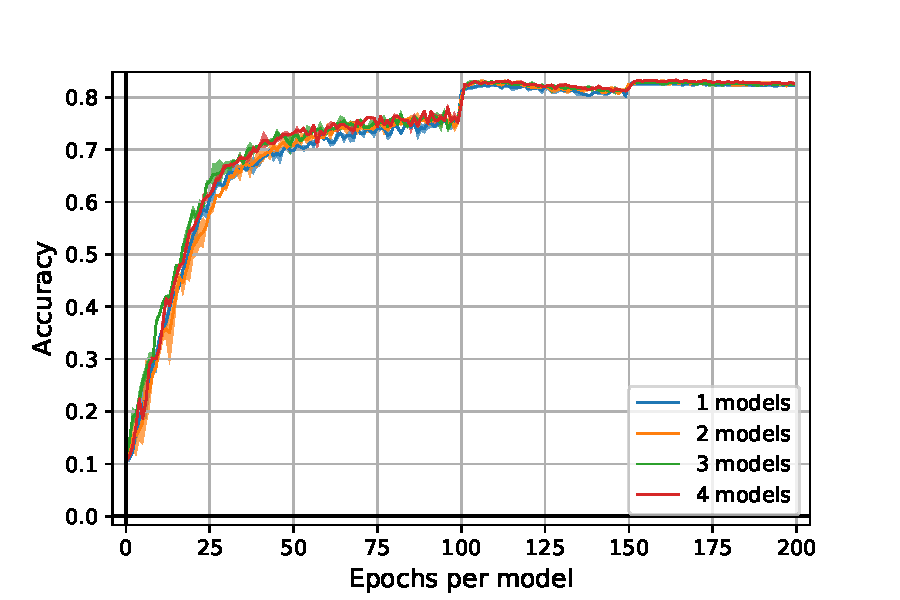
\includegraphics[width=0.24\textwidth]{Images/standard_acc_finalrun_ResNet18_1024_200_-1_bis.pdf}    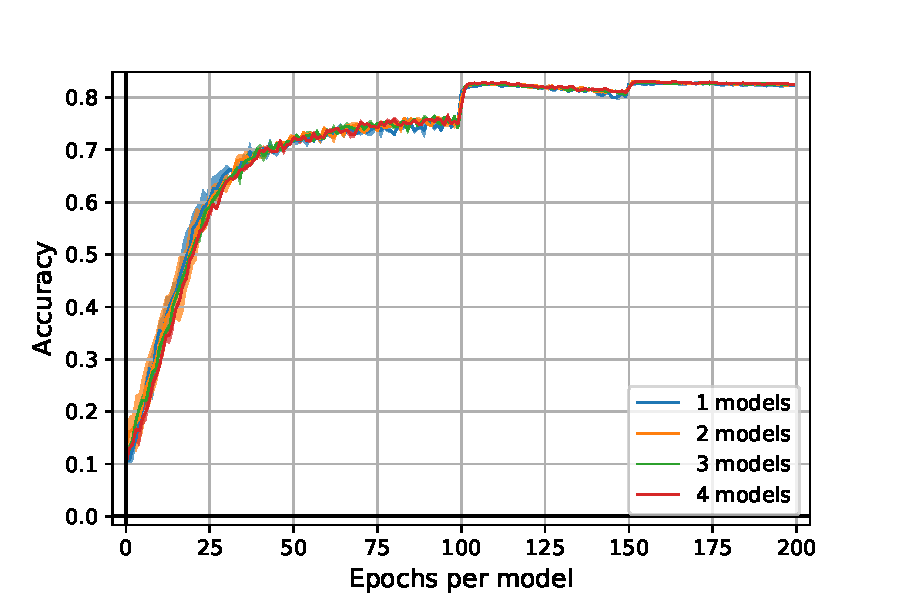
\includegraphics[width=0.24\textwidth]{Images/standard_acc_finalrun_ResNet18_1024_200_0.001_bis.pdf}
    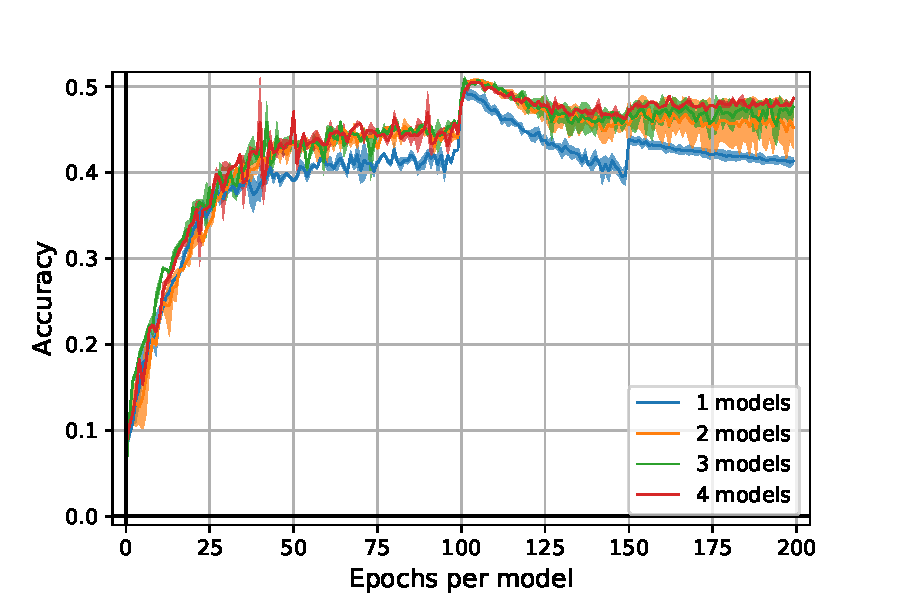
\includegraphics[width=0.24\textwidth]{Images/robust_acc_finalrun_ResNet18_1024_200_-1_bis.pdf}    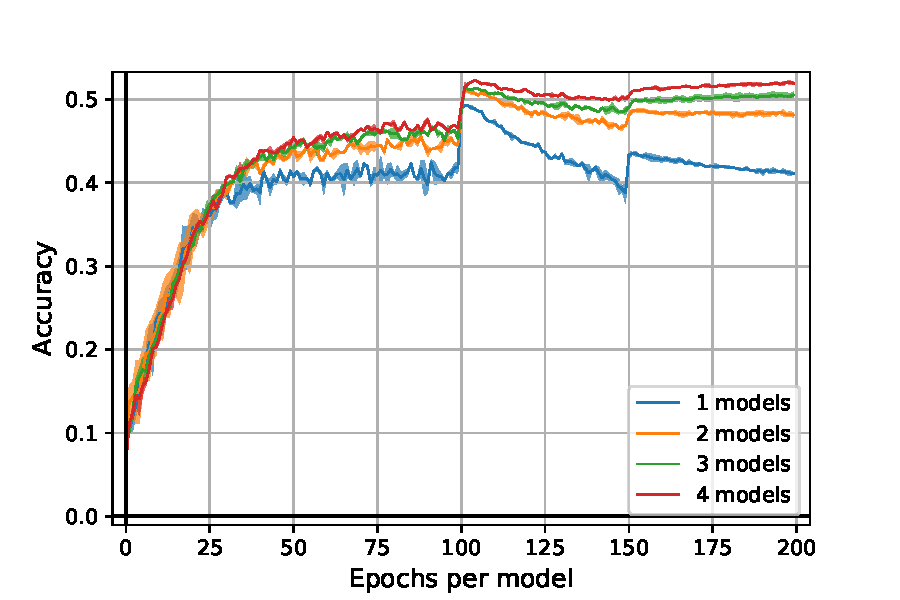
\includegraphics[width=0.24\textwidth]{Images/robust_acc_finalrun_ResNet18_1024_200_0.001_bis.pdf}
    \caption{On left and middle-left: Standard accuracies over epochs with respectively no regularization and regularization set to $\alpha=0.001$. On middle right and right: Robust accuracies for the same parameters against PGD attack with $20$ iterations and $\varepsilon=0.03$.}
    \label{fig:xp-regularization}
\end{figure}

\subsection{Additional Experiments on WideResNet28x10}

We now evaluate our algorithm on WideResNet28x10~\cite{ZagoruykoK16} architecture. Due to computation costs, we limit ourselves to $1$ and $2$ models, with regularization parameter set to $0.001$ as in the paper experiments section. Results are reported in Figure~\ref{fig:xp-wideresnet}. We remark this architecture can lead to more robust models, corroborating the results from~\cite{gowal2020uncovering}.
\begin{figure*}[!ht]
\begin{center}

\vskip 0.15in
 \begin{minipage}[ht!]{0.39\textwidth}
 \begin{scriptsize}
\begin{tabular}{c|c|ccc} 
\textbf{ Models} & \textbf{Acc. }&\textbf{$\textrm{APGD}_\textrm{CE}$}& \textbf{$\textrm{APGD}_\textrm{DLR}$} & \textbf{Rob. Acc.} \\ \hline
 1 & $85.2\%$ &	$49.9\%$ & $50.2\%$ & $48.5\%$ \\ 
 2 & $\bm{86.0\%}$ & $\bm{51.5\%}$ & $\bm{52.1\%}$ & $\bm{49.6\%}$\\ 

\end{tabular}
\end{scriptsize}
  \end{minipage}\begin{minipage}[!ht]{0.61\textwidth}
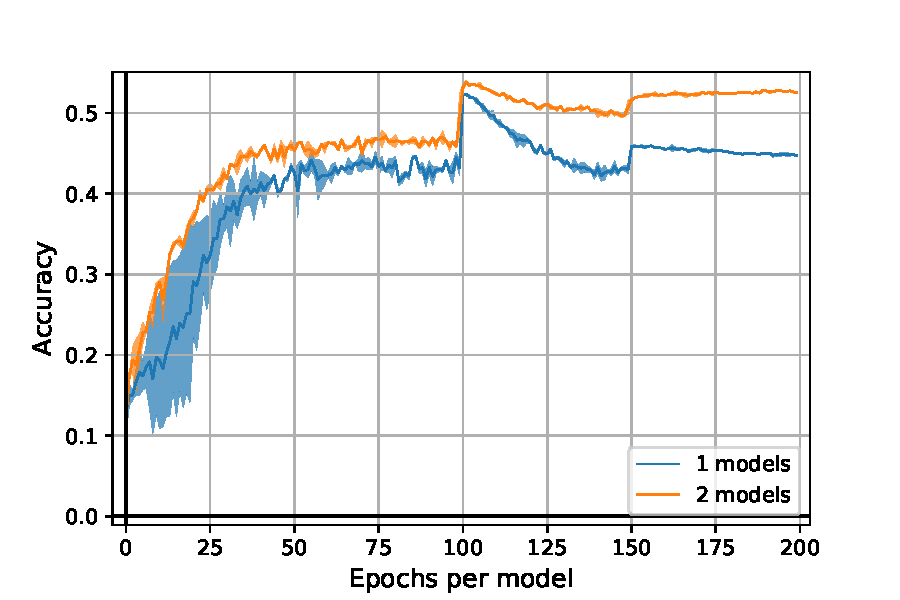
\includegraphics[width=0.49\textwidth]{Images/robust_acc_finalrun_WideResNet28x10_1024_200_0.001.pdf}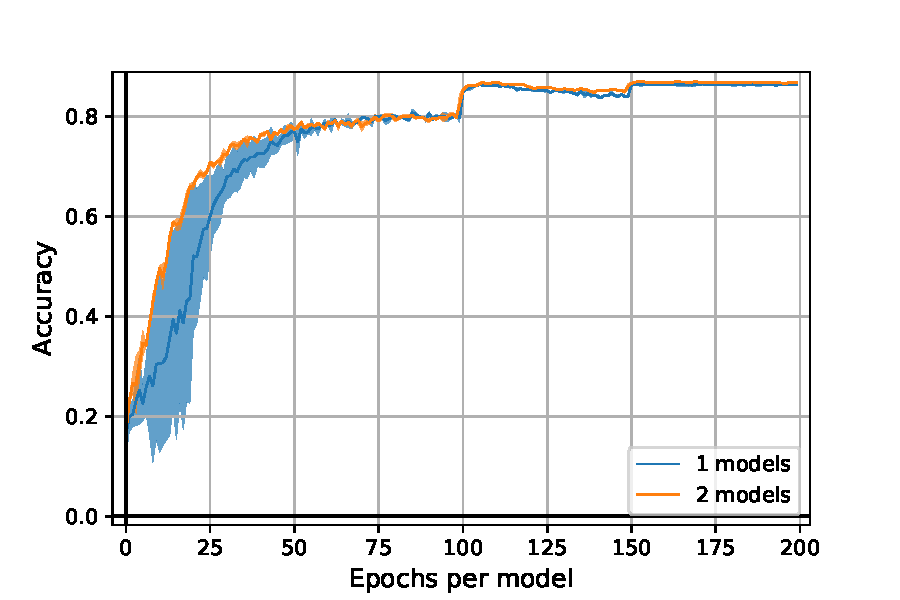
\includegraphics[width=0.49\textwidth]{Images/standard_acc_finalrun_WideResNet28x10_1024_200_0.001.pdf} 
  \end{minipage}
  
\caption{On left: Comparison of our algorithm with a standard adversarial training (one model) on WideResNet28x10. We reported the results for the model with the best robust accuracy obtained over two independent runs because adversarial training might be unstable. Standard and Robust accuracy (respectively in the middle and on right) on CIFAR-10 test images in function of the number of epochs per classifier with $1$ and $2$ WideResNet28x10 models. The performed attack is PGD with $20$ iterations and $\varepsilon=8/255$.}
\label{fig:xp-wideresnet}
\end{center}
\vspace{-0.1cm}
\end{figure*}


\subsection{Overfitting in Adversarial Robustness}
We further investigate the overfitting of our heuristic algorithm. We plotted in Figure~\ref{fig:overfitting} the robust accuracy on ResNet18 with $1$ to $5$ models. The most robust mixture of $5$ models against PGD with $20$ iterations arrives at epoch $198$, \emph{i.e.} at the end of the training, contrary to $1$ to $4$ models, where the most robust mixture occurs around epoch $101$. However, the accuracy against AGPD with 100 iterations in lower than the one at epoch $101$ with global robust accuracy of $47.6\%$ at epoch $101$ and $45.3\%$ at epoch 198. This strange phenomenon would suggest that the more powerful the attacks are, the more the models are subject to overfitting. We leave this question to further works.


\begin{figure*}[!ht]
\begin{center}
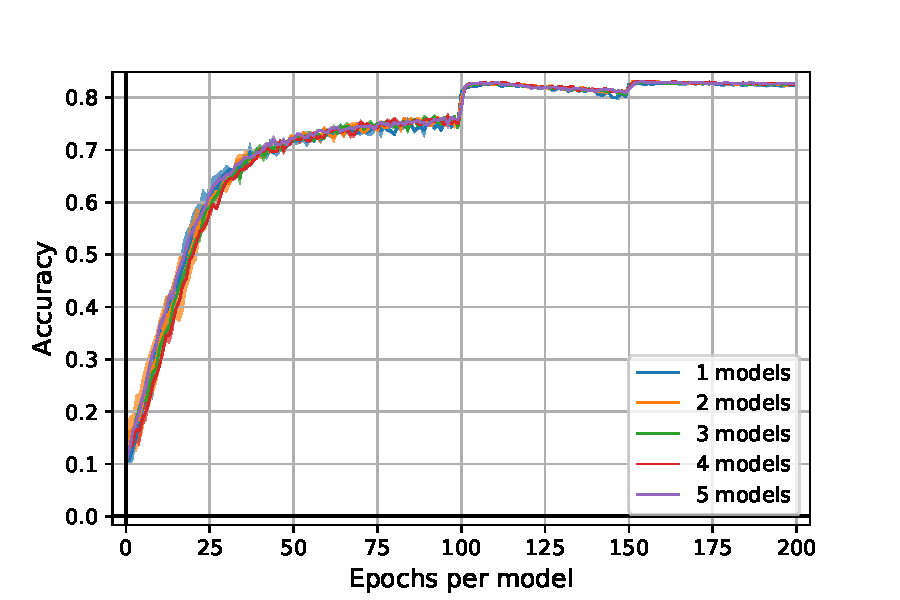
\includegraphics[width=0.49\textwidth]{Images/5_standard_acc_finalrun_ResNet18_1024_200_0.001.pdf}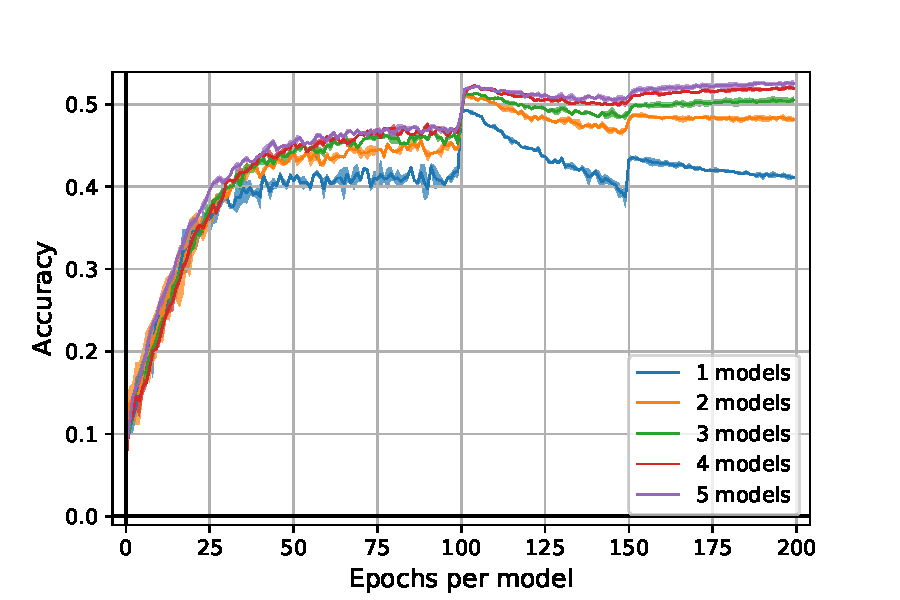
\includegraphics[width=0.49\textwidth]{Images/5_robust_acc_finalrun_ResNet18_1024_200_0.001.pdf} 

\caption{Standard and Robust accuracy (respectively on  left and on right) on CIFAR-10 test images in function of the number of epochs per classifier with $1$ to $5$ ResNet18 models. The performed attack is PGD with $20$ iterations and $\varepsilon=8/255$. The best mixture for $5$ models occurs at the end of training (epoch $198$).}
\label{fig:overfitting}
\end{center}
\end{figure*}
\subsection{Additional Results}
\label{sec:complements}
% \subsection{Equality of Standard Randomized and Deterministic Minimal Risks}
% \begin{prop}
% Let $\PP$ be a Borel probability distribution on $\mathcal{X}\times\mathcal{Y}$, and $l$ a loss satisfying Assumption~\ref{ass:loss}, then:
% \begin{align*}
%         \inf_{\mu\in\mathcal{M}^1_+(\Theta)} \risk(\mu) =\inf_{\theta\in\Theta} \risk(\theta)
% \end{align*}
% \end{prop}
% \begin{proof}
% It is clear that:         $\inf_{\mu\in\mathcal{M}^1_+(\Theta)} \risk(\mu) \leq \inf_{\theta\in\Theta} \risk(\theta)$. Now, let $\mu\in\mathcal{M}^1_+(\Theta)$, then:
% \begin{align*}
%     \risk(\mu)= \mathbb{E}_{\theta\sim\mu}(\risk(\theta))&\geq \essinf_\mu \mathbb{E}_{\theta\sim\mu} \left(\risk(\theta)\right)\\
%     &\geq\inf_{\theta\in\Theta} \risk(\theta).
% \end{align*}
% where $\essinf$ denotes the essential infimum.
% \end{proof}
% We can deduce an immediate corollary. 
% \begin{corollary}
% Under Assumption~\ref{ass:loss}, the dual for randomized and deterministic classifiers are equal.
% \end{corollary}

\subsection{Decomposition of the Empirical Risk for Entropic Regularization}

\begin{prop}
Let $\hat{\PP}:=\frac1N\sum_{i=1}^N \delta_{(x_i,y_i)}$. Let $l$ be a loss satisfying Assumption~\ref{ass:loss}. Then we have:
\begin{align*}
\frac{1}{N}\sum_{i=1}^N\sup_{x,~d(x,x_i)\leq\varepsilon}\mathbb{E}_{\theta \sim \mu}\left[l(\theta,(x,y))\right]=\sum_{i=1}^N\sup_{\QQ_i\in\Gamma_{i,\varepsilon}}\mathbb{E}_{(x,y)\sim \QQ_i,\theta \sim \mu}\left[l(\theta,(x,y))\right]
\end{align*}
where $\Gamma_{i,\varepsilon}$ is defined as : 
\begin{align*}
    \Gamma_{i,\varepsilon}:=\Big\{\QQ_i\mid~\int d\QQ_i=\frac{1}{N},~\int c_{\varepsilon}((x_i,y_i),\cdot) d\QQ_i=0\Big\}.
\end{align*}\end{prop}

\begin{proof}
This proposition is a direct application of Proposition~\ref{prop:dro_adv} for diracs $\delta_{(x_i,y_i)}$.
\end{proof}

% \subsection{On the NP-Hardness of Attacking a Mixture of Classifiers}
% In general, the problem of finding a best response to a mixture of classifiers is in general NP-hard. Let us justify it on a mixture of linear classifiers in binary classification: $f_{\theta_k}(x) = \langle \theta,x\rangle$ for $k\in [L]$ and $\bm{\lambda}=\mathbf{1}_L/L$. Let us consider the $\ell_2$ norm and $x=0$ and $y=1$. Then the problem of attacking $x$ is the following:
% \begin{align*}
%     \sup_{\tau,~\lVert \tau\rVert\leq\varepsilon} \frac{1}{L}\sum_{k=1}^L\mathbf{1}_{\langle \theta_k,x+\tau\rangle\leq0}
% \end{align*}
% This problem is equivalent to a linear binary classification problem on $\tau$, which is known to be NP-hard.




\subsection{Case of Separated Conditional Distribtions}
\begin{prop} Let $\mathcal{Y} = \{-1,+1\}$. Let $\PP\in\mathcal{M}^1_+(\mathcal{X}\times\mathcal{Y})$. Let $\varepsilon>0$. For $i\in\mathcal{Y}$, let us denote $\PP_i$ the distribution of $\PP$ conditionally to $y=i$. Let us assume that  $d_\mathcal{X}(\supp(\PP_{1+1}),\supp(\PP_{-1}))>2\varepsilon$. Let us consider the nearest neighbor deterministic classifier : $f(x) =  d(x,\supp(\PP_{+1}))-d(x,\supp(\PP_{-1}))$ and the $0/1$ loss $l(f,(x,y))=\mathbf{1}_{yf(x)\leq 0}$. Then $f$ satisfies both optimal standard and adversarial risks: $\risk(f)=0$ and $\riskadv^\varepsilon(f)=0$.
\end{prop}

\begin{proof} Let 
Let denote $p_i =\PP(y=i)$. Then we have
\begin{align*}
 \riskadv^\varepsilon(f)= p_{+1}\mathbb{E}_{\PP_{+1}}\left[\sup_{x',~d(x,x')\leq \varepsilon}\mathbf{1}_{ f(x')\leq 0}\right]+p_{-1}\mathbb{E}_{\PP_{-1}}\left[\sup_{x',~d(x,x')\leq \varepsilon}\mathbf{1}_{ f(x')\geq 0}\right]
\end{align*}
For $x\in \supp(\PP_{+1})$, we have, for all $x'$ such that $d(x,x')\neq 0$, $f(x')>0$, then: $\mathbb{E}_{\PP_{+1}}\left[\sup_{x',~d(x,x')\leq \varepsilon}\mathbf{1}_{ f(x')\leq 0}\right]=0$. Similarly, we have $\mathbb{E}_{\PP_{-1}}\left[\sup_{x',~d(x,x')\leq \varepsilon}\mathbf{1}_{ f(x')\geq 0}\right]=0$. We then deduce the result.
\end{proof}
